\documentclass[11pt,a4paper]{article}
%\pdfoutput=1
\usepackage{jheppub}
%\usepackage{dcolumn}
\usepackage{multirow}
\usepackage[section,subsection,subsubsection]{extraplaceins}
%\usepackage{afterpage}
%\usepackage{graphicx}
%\usepackage{caption}
%\usepackage{subcaption}
\usepackage[toc,page]{appendix}
\usepackage[final]{pdfpages}
\usepackage{filecontents}

\usepackage{graphicx}
%\usepackage{bookman}
%\usepackage[paper=A4,pagesize]{typearea}
%\usepackage[paper=A2,pagesize]{typearea}
%\usepackage{afterpage}
%\usepackage{lipsum}% dummy code

%% Hack to make math formulas bold in section titles
\makeatletter
\DeclareRobustCommand*{\bfseries}{%
  \not@math@alphabet\bfseries\mathbf
  \fontseries\bfdefault\selectfont
  \boldmath
}
\makeatother




\begin{document}

\title{The NEXT-DEMO++ detector}

%\author[a]{V.~Alvarez \thanks{Vicente.Alvarez@ific.uv.es}\emailAdd{vinny@gmail.com},}
\author[a]{F.~Monrabal,} \emailAdd{francesc.monrabal@ific.uv.es}
\author[a]{I.~Liubarsky,} \emailAdd{Igor.Liubarsky@ific.uv.es}
\author[a]{S.~C\'arcel,} \emailAdd{carcel@ific.uv.es}
\author[a]{J.J.~G\'omez-Cadenas,} \emailAdd{gomez@mail.cern.ch}
%\author[a]{A.~Martinez,} \emailAdd{Alberto.Martinez.Perez@ific.uv.es}
%\author[a]{J.~Rodriguez,} \emailAdd{Javier.Rodriguez@ific.uv.es}
%\author[b]{C.~Sofka,} \emailAdd{cjsofka@physics.tamu.edu}


\affiliation[a]{Instituto de F\'isica Corpuscular (IFIC), CSIC \& Universidad de Valencia \\
46980 Valencia, Spain}
%\affiliation[b]{ITexas A\& M University - Department of Physics and Astronomy
%College Station, 77843-7717 TX, 4242 TAMU, USA}

\abstract{}





\maketitle

%\tableofcontents

%\title[Sample title]{NEXT-DEMO++}

\section{Introduction}
NEXT-DEMO is a high-pressure xenon TPC contained within a cylindrical stainless-steel pressure vessel of diameter 30~cm and length 60~cm which was designed to operate at 10~bar. The TPC itself is defined by three metallic wire grids --- called \emph{cathode}, \emph{gate} and \emph{anode} --- which define the two active regions: the 30-cm long \emph{drift region}, between cathode and gate with a  drift field of typically 500~V~cm$^{-1}$; and the 5 mm long \emph{EL region}, between gate and anode.  The electric field is created by supplying a large negative voltage to the cathode, then degrading it using a series of metallic rings of 30 cm diameter spaced 5 mm and connected via 0.5~G$\Omega$ resistors (shown in figure~\ref{fig:TPC}).  The gate is at negative voltage so that a moderate electric field of typically 2$\mathrm{kV~cm^{-1}~bar^{-1}}$ --- is created between the gate and the anode, which is at ground. A set of six panels made of PTFE (Teflon) coated with tetraphenyl-butadiene (TPB) are mounted inside the electric-field cage forming a \emph{light tube} of hexagonal cross section with an apothem length of 8~cm. 


%%%%%%%%%%
\begin{figure}
\centering
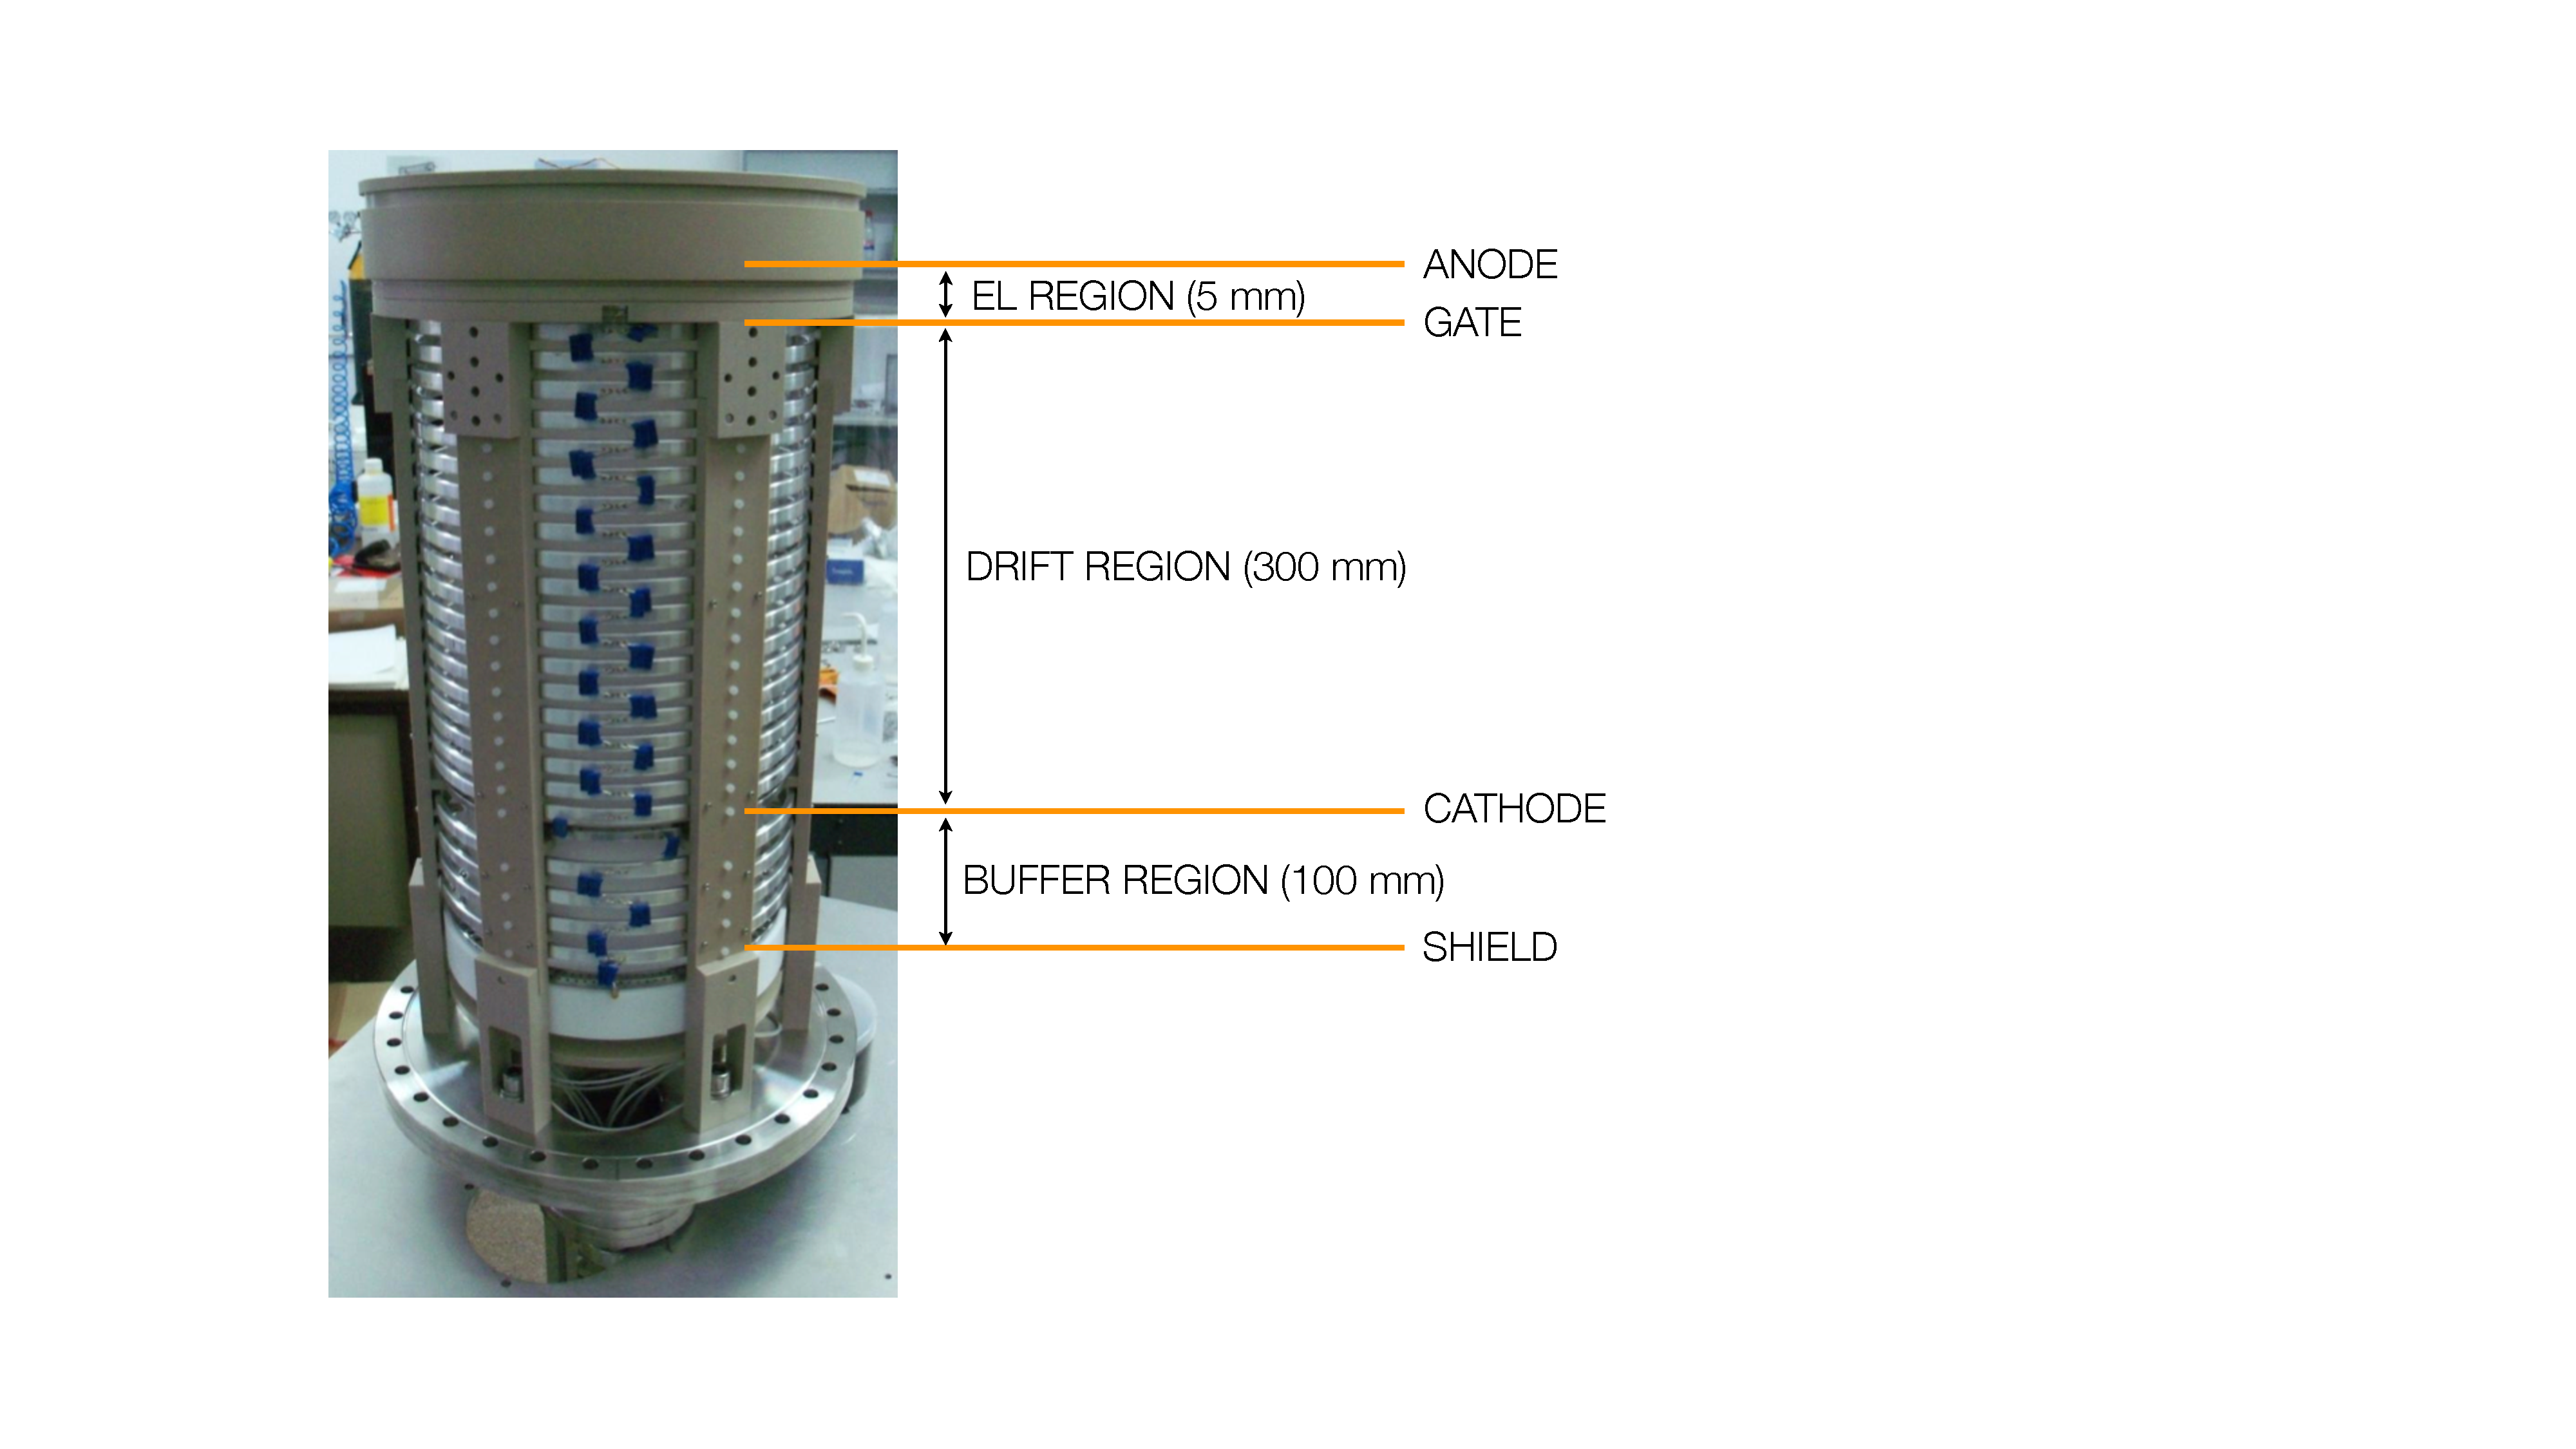
\includegraphics[width=0.75\textwidth]{img/FieldCage.pdf}
\caption{External view of the time projection chamber mounted on one end-cap. The approximate positions of the different regions of the TPC are indicated.} \label{fig:TPC}
\end{figure}
%%%%%%%%%%


The NEXT-DEMO detector has been operating continuously at IFIC (Figure \ref{fig:cleanroom} shows the NEXT-DEMO detector in the experimental are at IFIC ) during the last three years (2011-2014). Its operation and results has been crucial to fully demonstrate the capabilities of the NEXT technology for the search of the neutrinoless double beta decay process. Furthermore, the operation, devoid of any significant incidence has shown the robustness of the system. 

%%%%%%%%%%
\begin{figure}
\centering
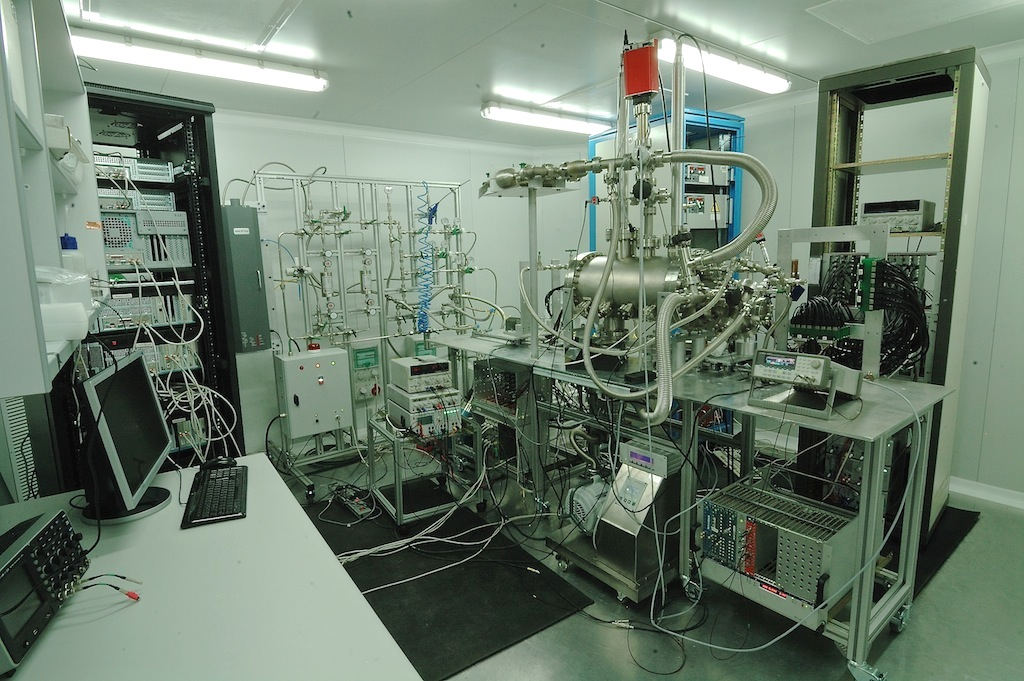
\includegraphics[width=0.75\textwidth]{img/NextDemo_cleanroom.jpg}
\caption{Picture of the NEXT-DEMO detector in the experimental area at IFIC with all the different systems needed for its operation: Gas system, High voltage modules and electronics.} \label{fig:cleanroom}
\end{figure}
%%%%%%%%%%

We propose to use NEXT-DEMO to demonstrate the possibility to operate the NEXT experiment inside a magnetic field of relatively high intensity ($\sim$ 0.5 Tesla). Recent Monte Carlo studies show that the separation between signal and background in the search for neutrinoless double beta decay can be improved by one order of magnitude measuring the sign of the electrons emitted in the decay. However, operation in magnetic field requires a number of upgrades to the current technology (including substituting the PMTs used to measure the event energy by large-area SiPMs and the use of small amounts of CO$_2$ to reduce transverse and longitudinal diffusion) which must be demonstrated experimentally.  

Consequently, we would like to carry out a series of tests at CERN. We propose to place an upgraded version of  NEXT-DEMO detector inside the HARP magnet (TPC90) and operate the detector in various configurations of pressure and magnetic field in order to understand operation in magnetic field and to confirm our Monte Carlo results.
We propose to carry out those tests in 2016, with a possible extension to 2017. 

This document describes at some depth the system that we propose to bring to CERN, including safety aspects. 

%%%%%%%%%%%%%%%%%%%%%%%%%%%%%%%%%%%%%%%%%%%%%%%%%%%%%%%%%%%%
\section{Pressure vessel} \label{sec:PressureVessel}
%%%
The pressure vessel of NEXT-DEMO, shown in figure~\ref{fig:Vessel}, is a stainless-steel (grade 304L) cylindrical shell, 3 mm thick, 30 cm diameter and 60 cm length, welded to CF flanges on both ends. The two end-caps are 3-cm thick plates with standard CF knife-edge flanges. Flat copper gaskets are used as sealing. The vessel was certified to 10 bar operational pressure. It was designed at IFIC and built by Trinos Vacuum Systems, a local manufacturer. Additional improvements --- including the support structure and a rail system to open and move the end-caps --- have been made using the mechanical workshop at IFIC.

%%%%%%%%%%
\begin{figure}
\centering
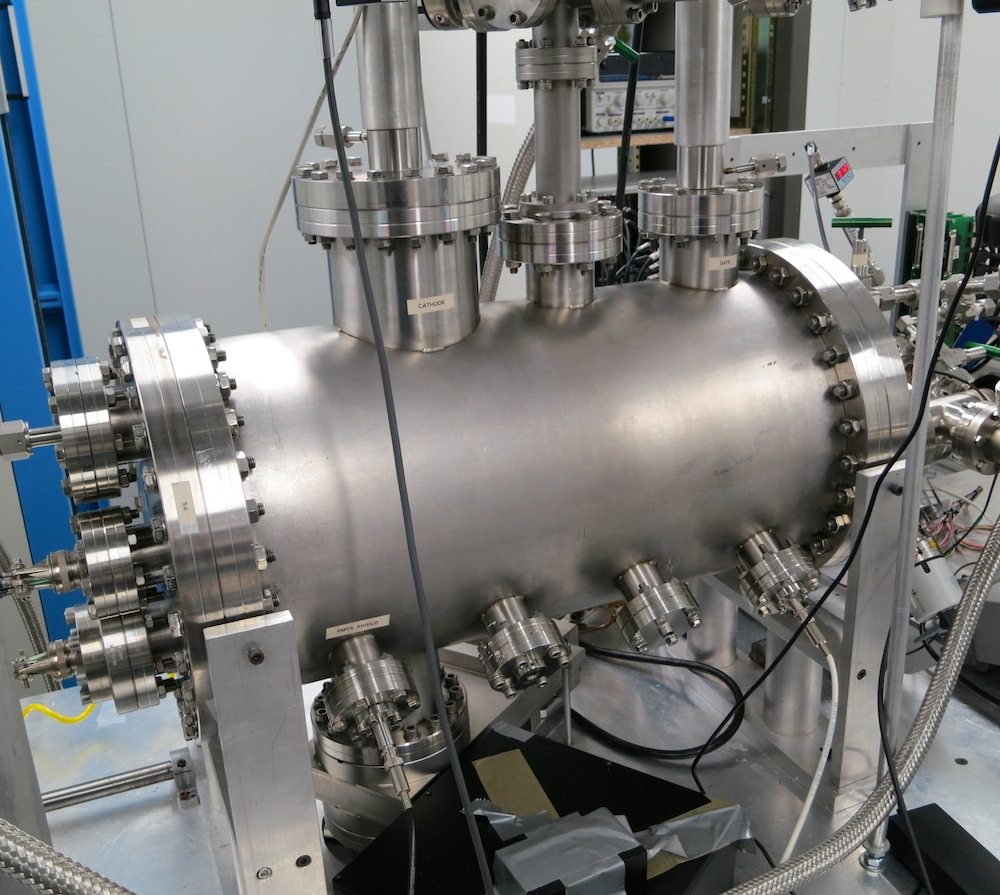
\includegraphics[scale=0.9]{img/VesselCloseup.jpg}
\caption{The pressure vessel of NEXT-DEMO.} \label{fig:Vessel}
\end{figure}
%%%%%%%%%%

The side of the chamber includes 8 CF40 half-nipples. One set of 4 is located in the horizontal plane while the other is displaced towards the underside with respect to the first set by $60^\circ$. These contain radioactive source ports used for calibration of the TPC. The ports are made by welding a 0.5 mm thick blank SS plate onto a 12 mm OD pipe on a CF40 liquid feedthrough. On top of the vessel and along the vertical plane there are three additional half-nipples (CF130, CF67 and CF80) used for high-voltage input and connection to a mass spectrometer (through a leak valve). On the opposite side, at the bottom, a CF100 port connects the pressure vessel to the vacuum pumping system. A guillotine valve closes this connection when the vessel is under pressure. The end-caps include several CF ports for the connections to the gas recirculation loop and for the feedthroughs (power and signal) of the PMT planes.

%%%%%%%%%%%%%%%%%%%%%%%%%%%%%%%%%%%%%%%%%%%%%%%%%%%%%%%%%%%%
\section{Gas system} \label{sec:GasSystem}

The functions of the gas system of NEXT-DEMO are the evacuation of the detector, its pressurization and depressurization with xenon (and argon), and the recirculation of the gas through purification filters. A schematic of the system is shown in figure~\ref{fig:GasSystem}.

%%%%%%%%%%
\begin{figure}[tbh]
\centering
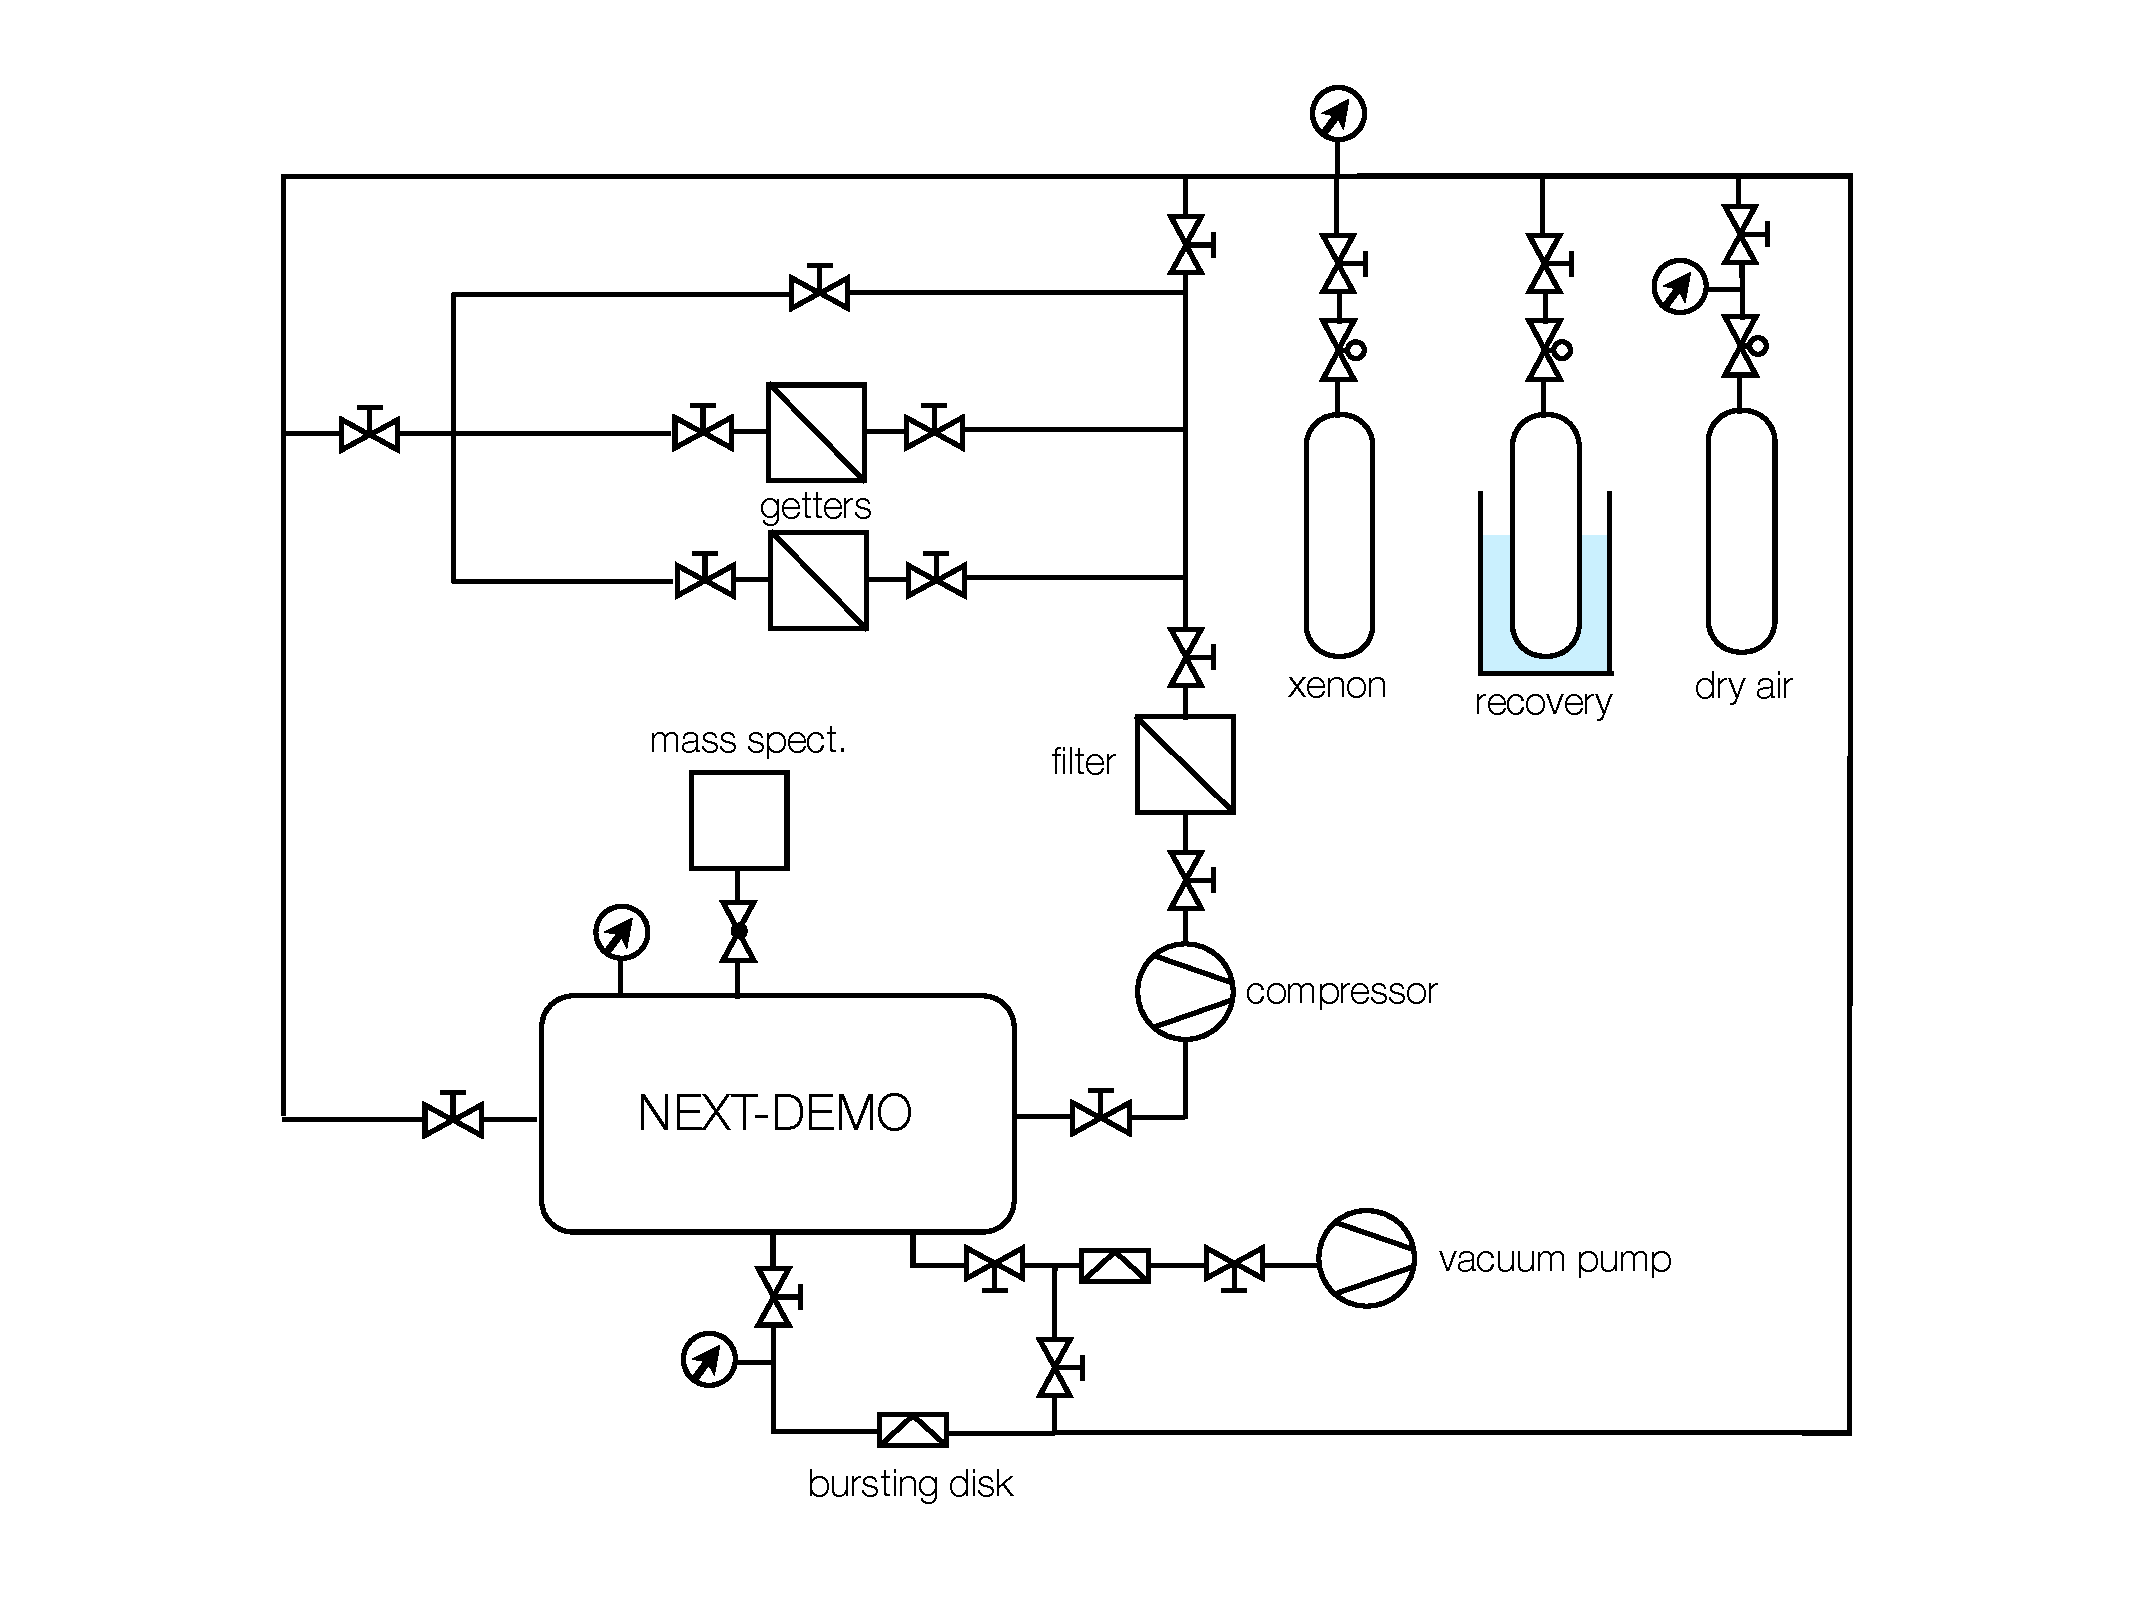
\includegraphics[width=\textwidth]{img/GasSystem.pdf}
\caption{Simplified schematic of the gas system of NEXT-DEMO.} \label{fig:GasSystem}
\end{figure}
%%%%%%%%%%

The standard procedure during normal operation of the detector starts with the evacuation of the vessel to vacuum levels around $10^{-5}$~mbar. The detector is then filled with xenon gas to pressures up to 10 bar. The xenon can be cryogenically recovered to a stainless-steel bottle (Fig. \ref{fig:RecoB}) connected to the gas system by simply immersing this in a dewar filled with liquid nitrogen. The gas flows inside the bottles and freezes there.
%The pressure regulator of the bottle is fully opened to allow the xenon gas to flow inside it (due to the temperature difference) and freeze.

%%%%%%%%%%
\begin{figure}[tbh]
\centering
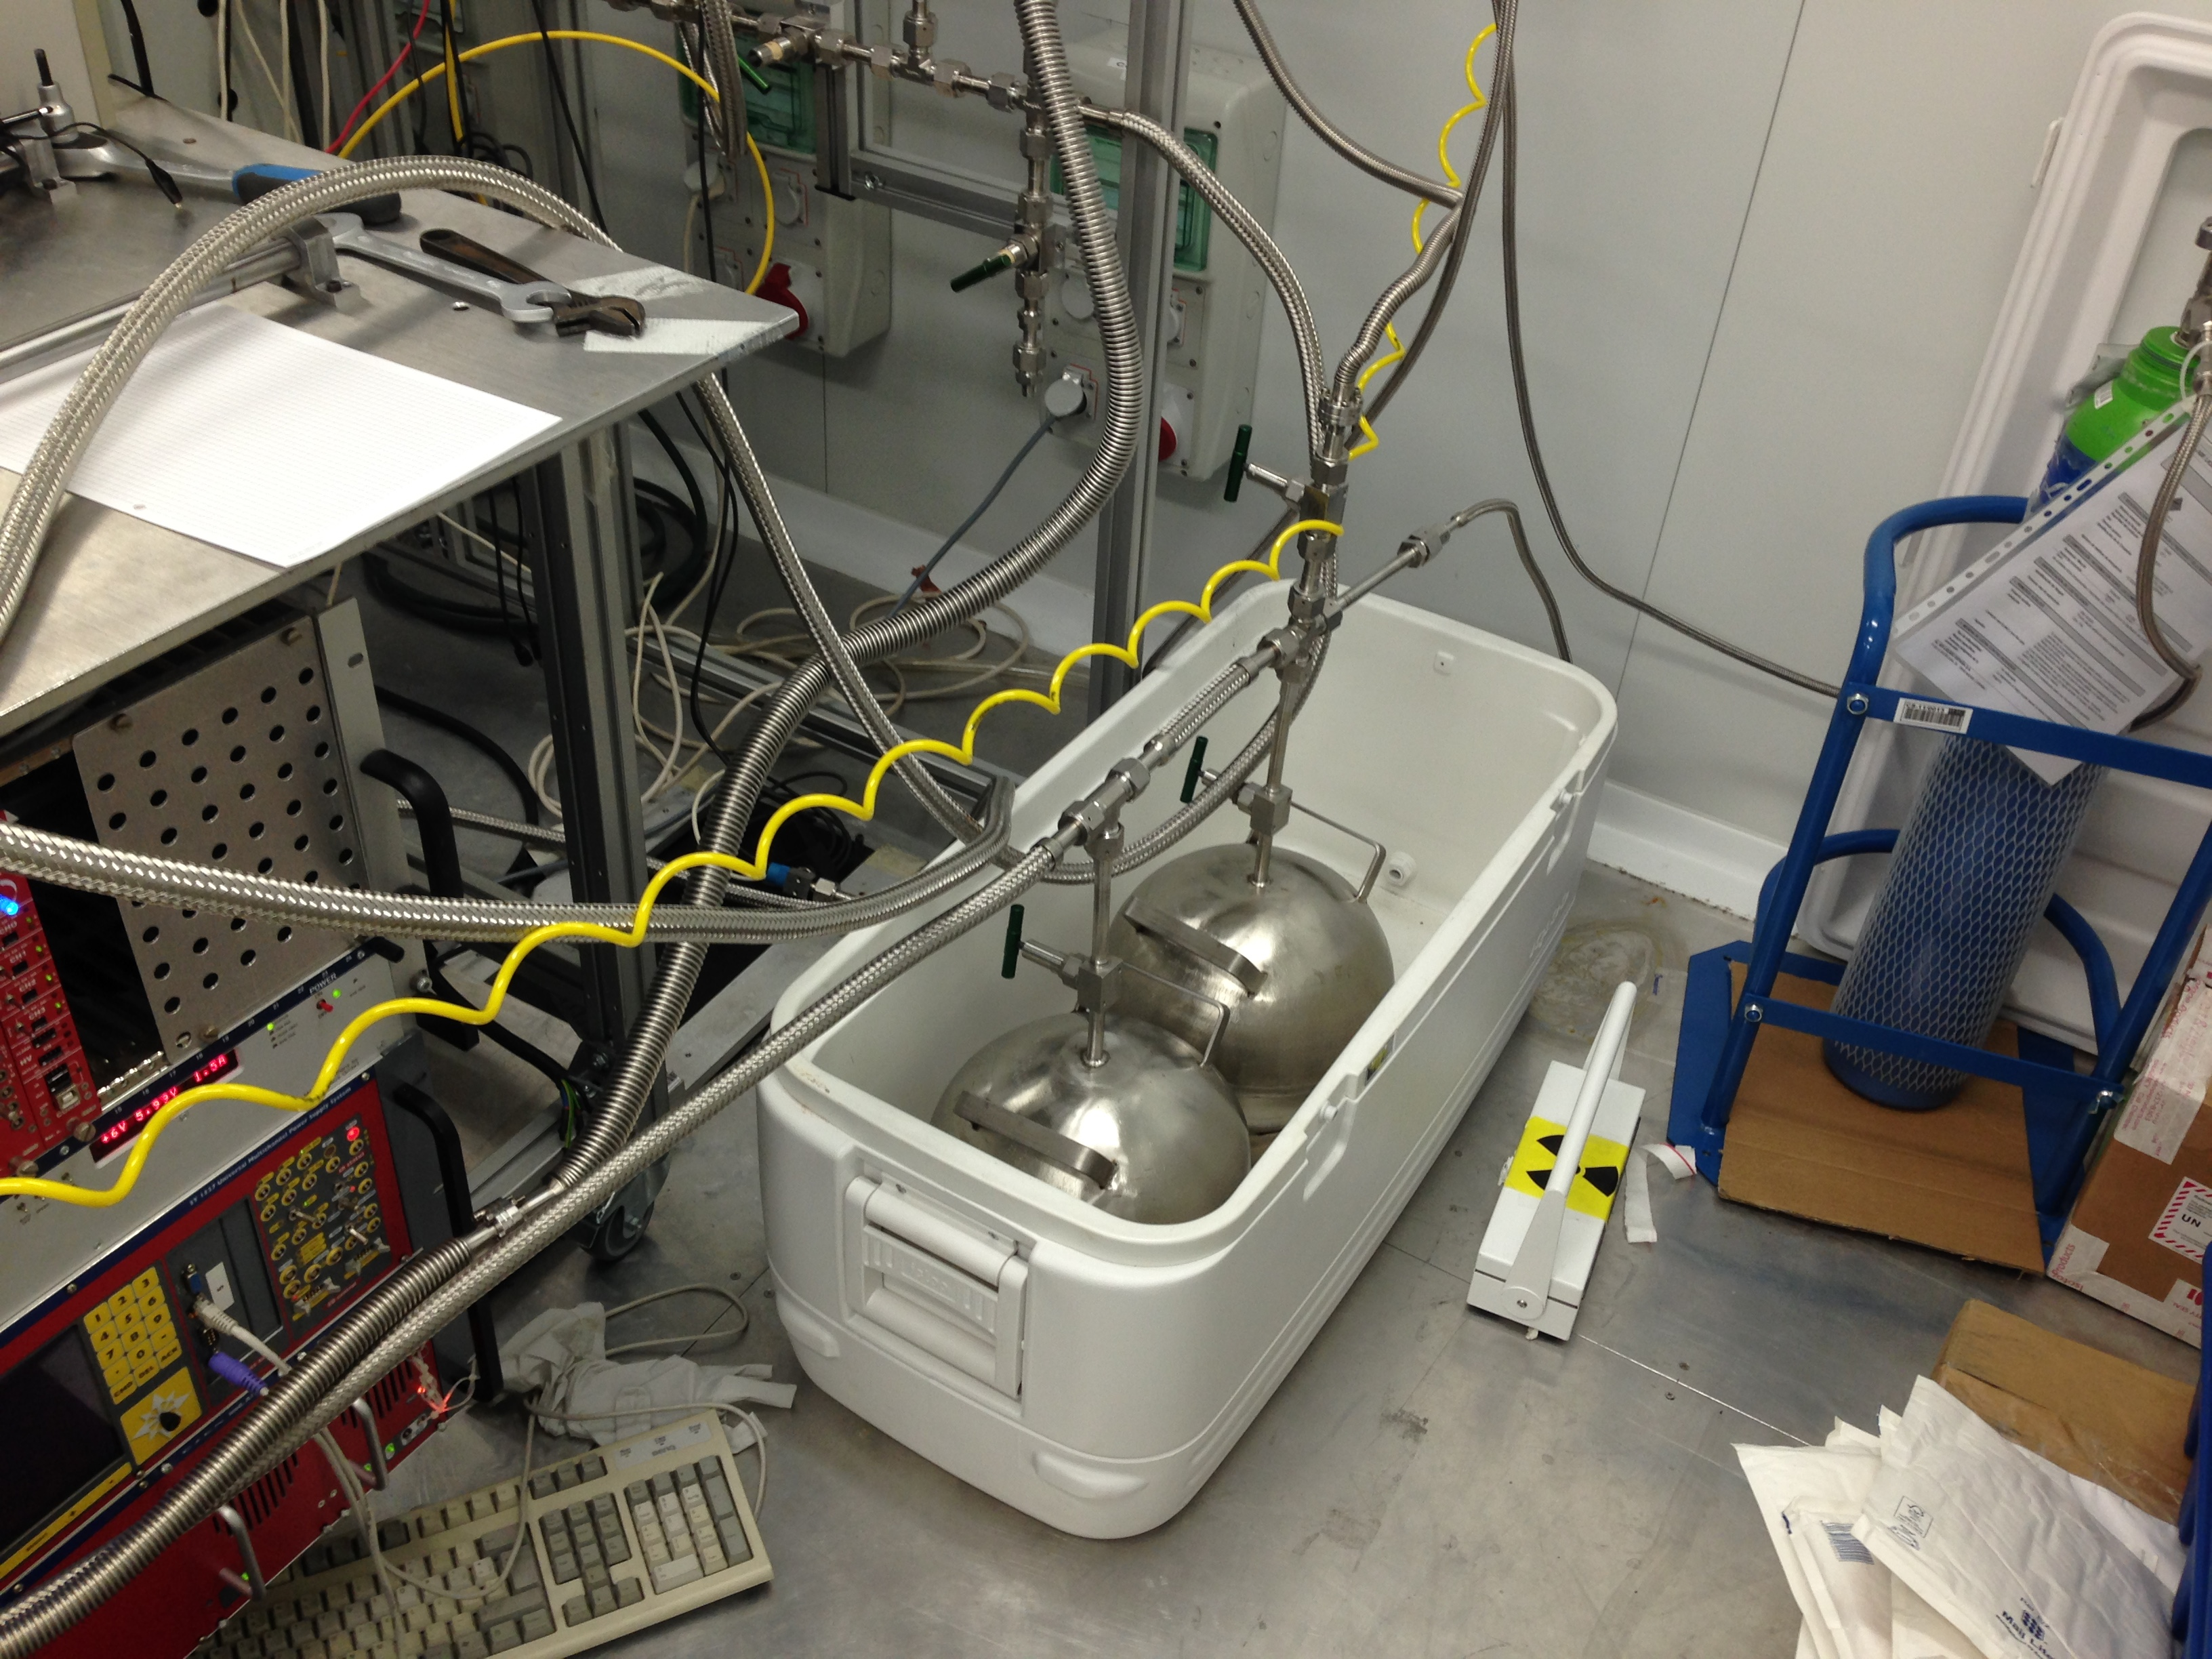
\includegraphics[width=\textwidth]{img/recoverybottle.jpg}
\caption{Stainless steel bottles used for cryogenic recovery of the Xenon} \label{fig:RecoB}
\end{figure}
%%%%%%%%%%



The vacuum pumping system consists of a roughing pump (Edwards XDS5 scroll vacuum pump) and a turbo molecular pump (Pfeiffer HiPace 300). Vacuum pressures better than $10^{-7}$~mbar have been obtained after pumping out the detector for several days. The recirculation loop is powered by an oil-less, single-diaphragm compressor (KNF PJ24999-2400) with a nominal flow of 100 standard liters per minute. This translates to 
an approximate flow of 10 liters per minute at 10 bar, thus recirculating the full volume of NEXT-DEMO ($\sim45$~L) in about 5 minutes. The gas system is equipped with both room-temperature (SAES MC50) and heated \emph{getters} (SAES PS4-MT15) that remove electronegative impurities (O$_{2}$, H$_{2}$O, etc.) from the xenon. All the gas piping, save for the inlet gas hoses and getter fittings, are $1/2$ inch diameter with VCR fittings. A set of pressure relief valves (with different settings for the various parts of the system) and a burst disk in the vacuum system protect the equipment and personnel from overpressure hazards.

The operation of the gas system (Fig. \ref{fig:GasSystem2}) has been, in general, very stable. The detector has run without interruption for long periods with no leaks and continuous purification of the gas. However, one major leak occurred when the diaphragm of the recirculation pump broke, causing the loss of the xenon volume contained in the chamber. This led to the installation of an emergency mechanism that, in the event of pressure drop, automatically closes those valves connecting the pump to the rest of the gas system. Since installation, only one major failure has taken place which the emergency system isolated without loss of gas.  Micro-leaks, on the level of 0.005 bar per day, due to bad connections in the gas system have also been detected making it necessary to introduce additional xenon to maintain pressure. The micro-leaks where found and properly repaired allowing for a stable detector operation in the last year.

%%%%%%%%%%
\begin{figure}[tbh]
\centering
\includegraphics[width=\textwidth]{img/GasSystem2.jpg}
\caption{Picture of the Gas system used in the NEXT-DEMO detector.} \label{fig:GasSystem2}
\end{figure}
%%%%%%%%%%


Several improvements to the initial design of the gas system have been made thanks to the initial data runs. These include the recognition of the importance of reliability of the main pump as well as the decision to use hot getters as the main gas purification stage due to their negligible emission of radon compared to that of room-temperature getters.

\subsection{Cryo-recovery protocol}

When the gas system needs to be stopped for an intervention in the detector the gas Xenon needs to be recovered and saved. The way of recovering the Xenon from the vessel and the gas system is with cryogenics.

NEXT-DEMO gas system has two spherical bottles specially designed for this use (see attachements) that are connected to the vessel and to the gas system. The bottles are placed in a thermally insolated container that is filled with liquid nitrogen until it reaches (approx.) half of the height of the bottles. Once the nitrogen stops boiling we open the corresponding valve to the part of the system that we want to recover, vessel or gas system. It is also possible to have both open at the same time if needed. Then the Xenon flows into the recovery bottles where it frezzes.

Once the pressure in the vessel/gas system is stable at ~0.03 absolute bar the bottles are full and we close them. Then we need to wait for the liquid nitrogen to evaporate.



\subsection{Gas Mixtures}

For the updgrade of NEXT-DEMO++ we will need to operate the detector with a mixture of Xenon with other gas. The gas choosen as a first option is CO$_2$. This gas give us all the advantages of the gas mixtures (improvement in drift velocity, reduction of diffusion,...) at concentrations smaller than 1\% . In order to control the concentration of CO$_2$ the gas system will need a small upgrade consisting in two flow meters and a small bottle of CO$_2$.


\subsection{Technical and safety specifications}

The gas system is made up of standard components. The Getters and the compressor carry CE marks.

Swagelock components do not carry a CE mark. However, all Swagelock
components used comply with the requirement of Article~3, Paragraph~3 of the PED Directive \mbox{(97/23/EC)} and in accordance with that section do not carry a CE mark. Notwithstanding, we can included all the certificates.

The complete list of parts with the associated part numbers is given in attachment "VALCI-MONTI-195". We have also selected a list of major components that is given below, in which we have omitted explicit listing of the standard components such as elbows and similar coupling as they are too numerous and being all manufactured by Swagelock comply with the above mentioned PED directive.


%bellow. We have omitted explicit listing of the standard components such as elbows and similar coupling as they are too numerous and being all manufactured by Swagelock comply with the above mentioned PED directive.
%
\begin{itemize}

\item  28 $\times$ 1/2Ó VCR valves SS/8BG-VCR
\item  3 $\times$ 1/4Ó VCR valves 6LVV-DPHVR4-P1
\item  2 $\times$ 1/4Ó VCR valves SS-4BC-VCR
\item  3 $\times$ regulators KPR1JRFX27A20000

\item  2 $\times$  Cold getters SAES Pure Gas MC450-902
\item  1 $\times$  Hot getter SASE Pure Gas PS4-MT15-R2

\item  Compressor: 1 $\times$ KNF PJ24999-2400
\end{itemize}


Non standard components are:
The Vessel and the Stainless steel recovery bottles which were specifically designed and tested for NEXT. The calculations and test document are included in the attachment document to this one.




%\subsection{Technical and safety specifications}
%
%The gas system has been built and assembled by Swagelock. All the different parts have the safety certificate for pressure operation in the attached documents.


\section{Field Cage} \label{sec:Introduction} 


The NEXT-DEMO field cage is designed to provide an homogeneous and uniform electric field inside the active volume of the NEXT-DEMO detector. To achieve this different parts have to be designed, constructed and assembled. The different components of the the field cage project are:
\begin{itemize}
\item Drift region.
\item Buffer.
\item High voltage feedthroughs.
\item Cathode grid.
\item Electroluminescent region.
\end{itemize}


The main safety issues are related with the high voltage that we need to apply to the detector. In that sense, the entire detector and all of its metallic components are to be grounded for safety. The grounding points will provide path of least resistance to any stray transients resulting from HV discharges as is common for operation of HV equipment. Moreover, the currents will be small ($\mathcal{O}(\mu A)$) due to the large value of the resistors involved.

\subsection{Drift region}

The drift regions needs to create a moderate (300-600V/cm) but very homogeneous electric field. This is done using copper rings connected 10$G\Omega$ resistors. Figure \ref{fig:drift1} shows an example of the rings used for the NEW detector, the concept used in DEMO will be the same.

\begin{figure}[h!]
\centering
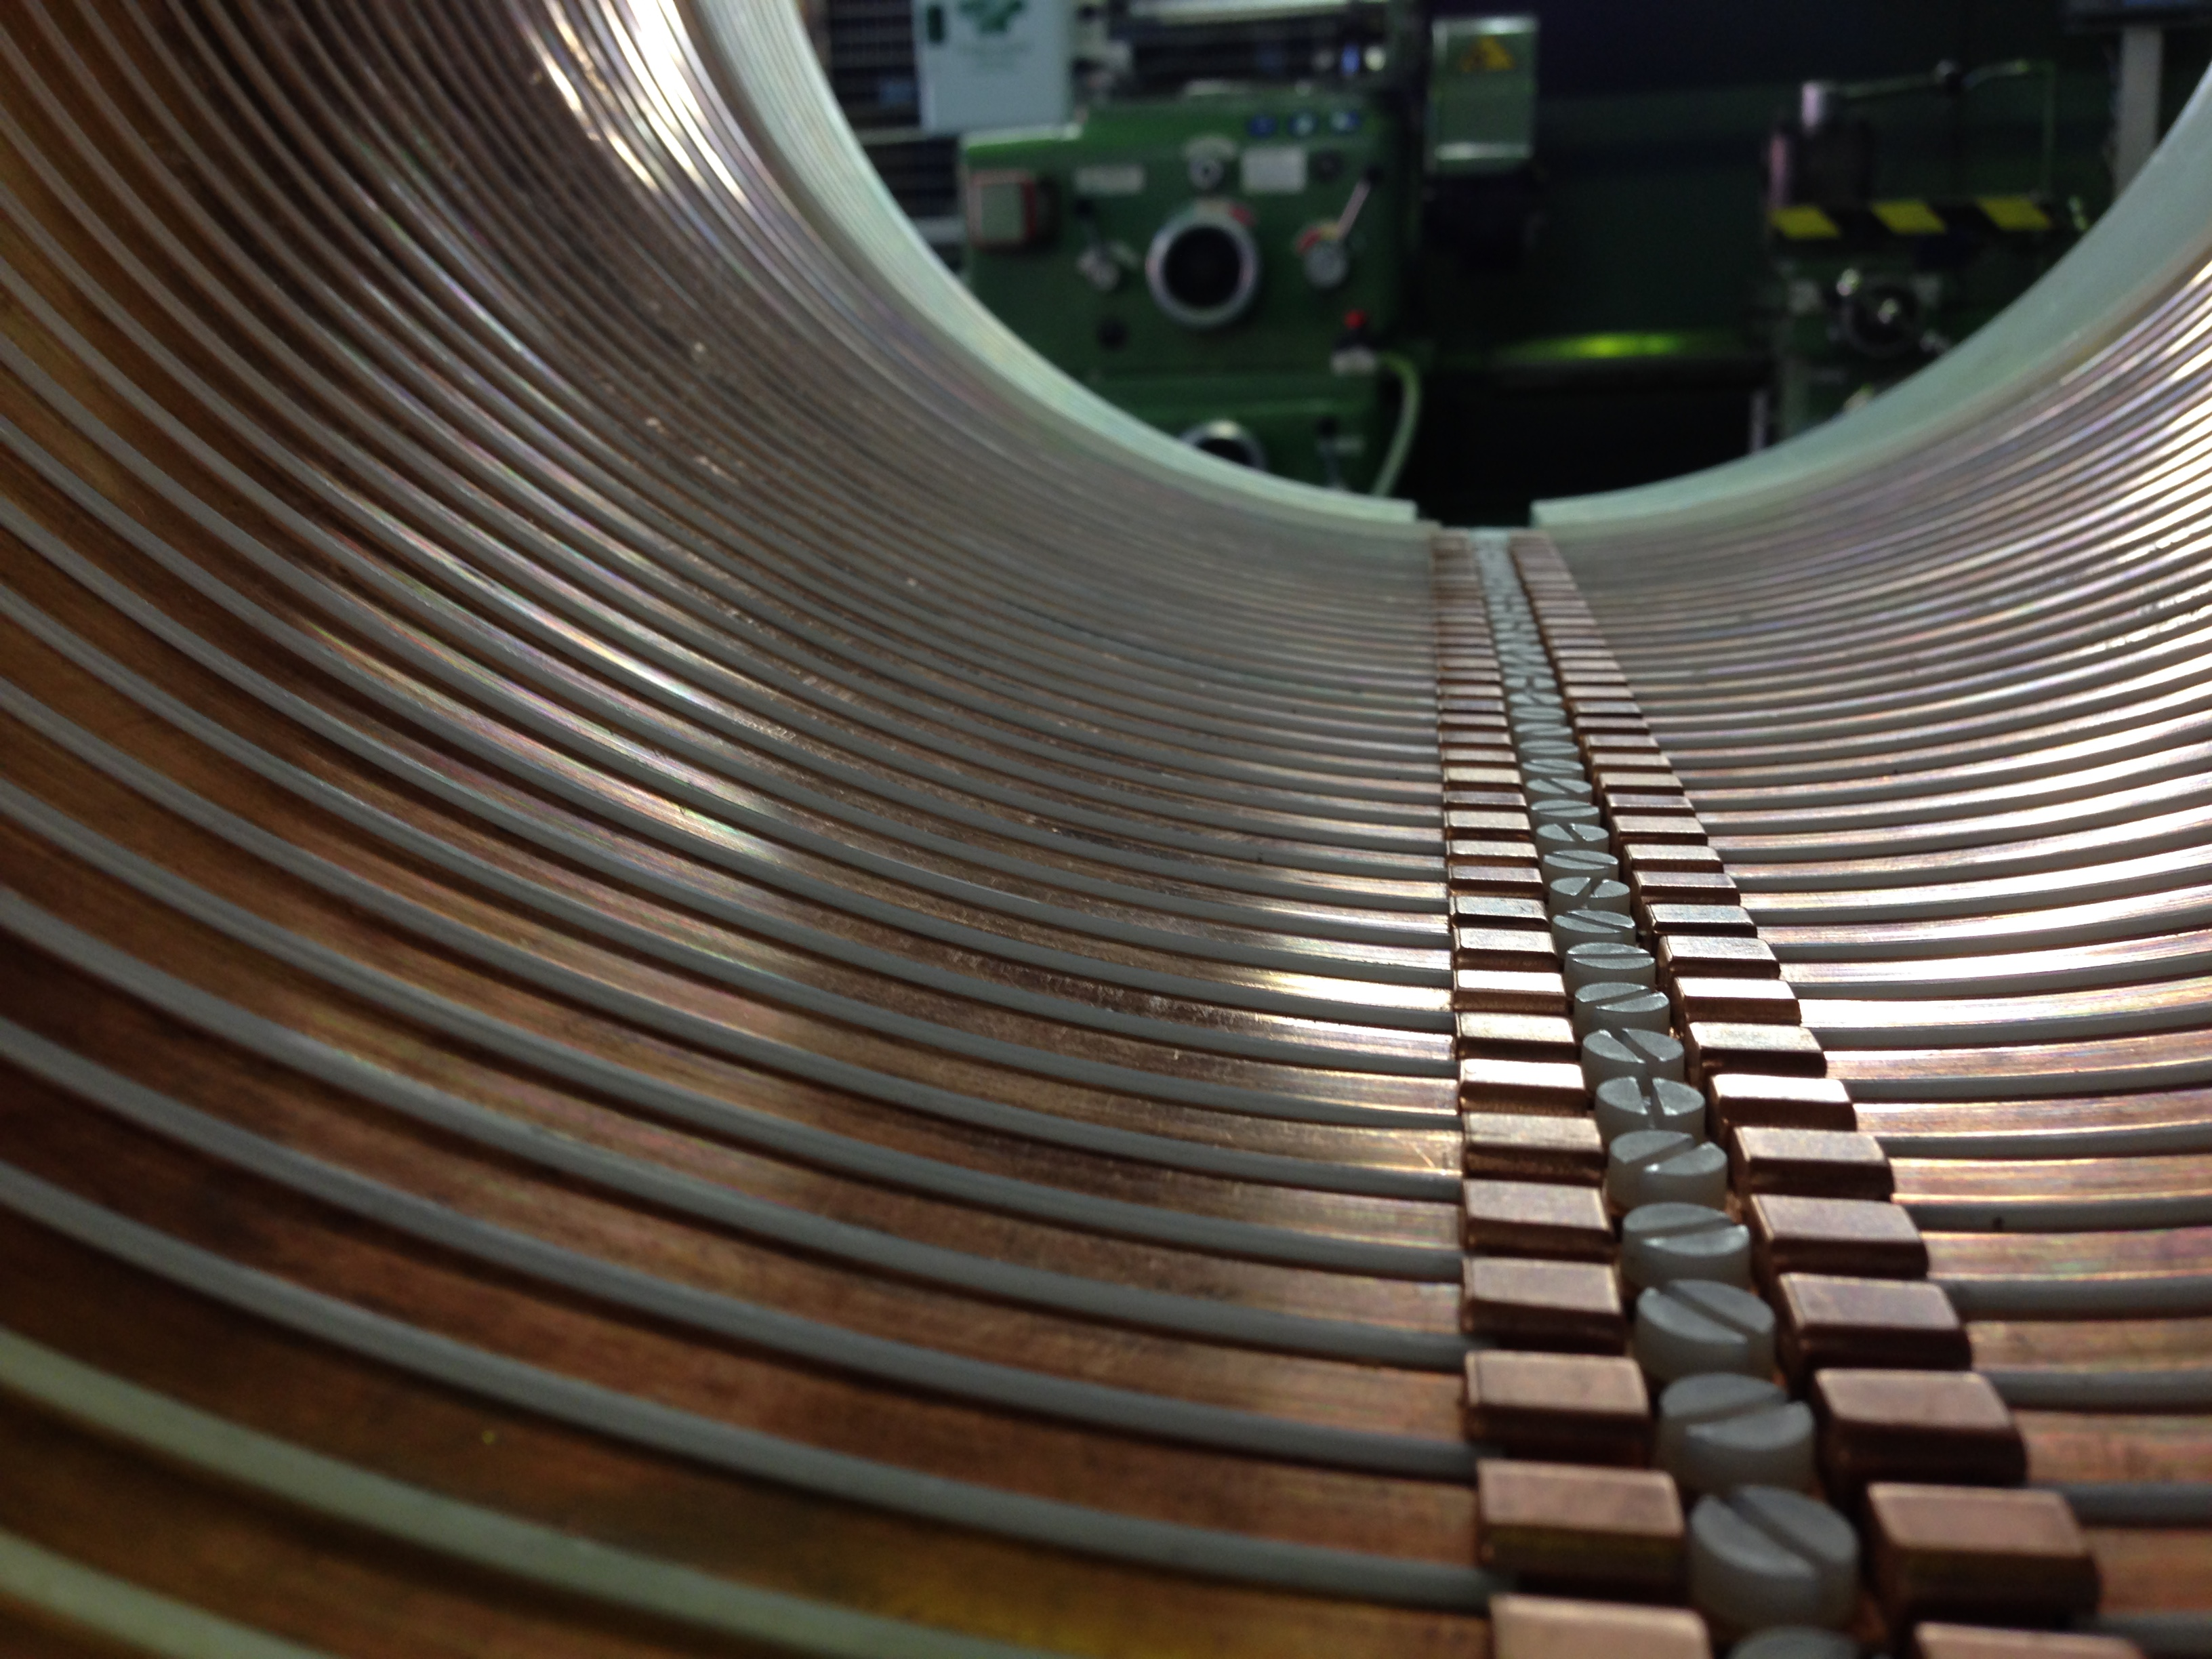
\includegraphics[height=8cm]{img/IMG_0246.JPG}
\caption{Detail of the copper rings in the drift region.} \label{fig:drift1}
\end{figure}


\subsection{Buffer region}

In order to protect the PMTs' windows from the cathode voltage safely a certain distance is needed. This space is what we call buffer region. In the current design the buffer region consists in a structure made completely with High Density Polyethilene (HDPE). The electric field in this region is much higher than in the drift region, as much as 5kV/cm, and it can result in sparks in different parts of the detector. For that reason the buffer has been extensively tested and has demostrated to be very robust and stable.

%A first test using a small set-up has shown promising result. The buffer region held the voltage until the High Voltage Feedthrough used for the test started sparking (Fig. \ref{fig:buff1}).
%
%\begin{figure}[h!]
%\centering
%\includegraphics[width=0.45\textwidth]{img/buff1.JPG}
%\caption{Detail of the buffer region test made with High Density Polyethilene (HDPE). Carbon tracks appear to the outside of the HDPE but no carbon tracks are visible in the inside of the buffer region. } \label{fig:buff1}
%\end{figure}
%
%A more extensive and realistic test will be performed using the NEXT-DEMO detector. For conducting this test we will replace the current NEXT-DEMO field cage by a small scale field cage of NEW (Fig. \ref{fig:bufftest}) using also the same HVFT that we want to use for NEW. In this way we would be able to test time both the buffer region and the HVFT in a more realistic situation.
%
%\begin{figure}[h!]
%\centering
%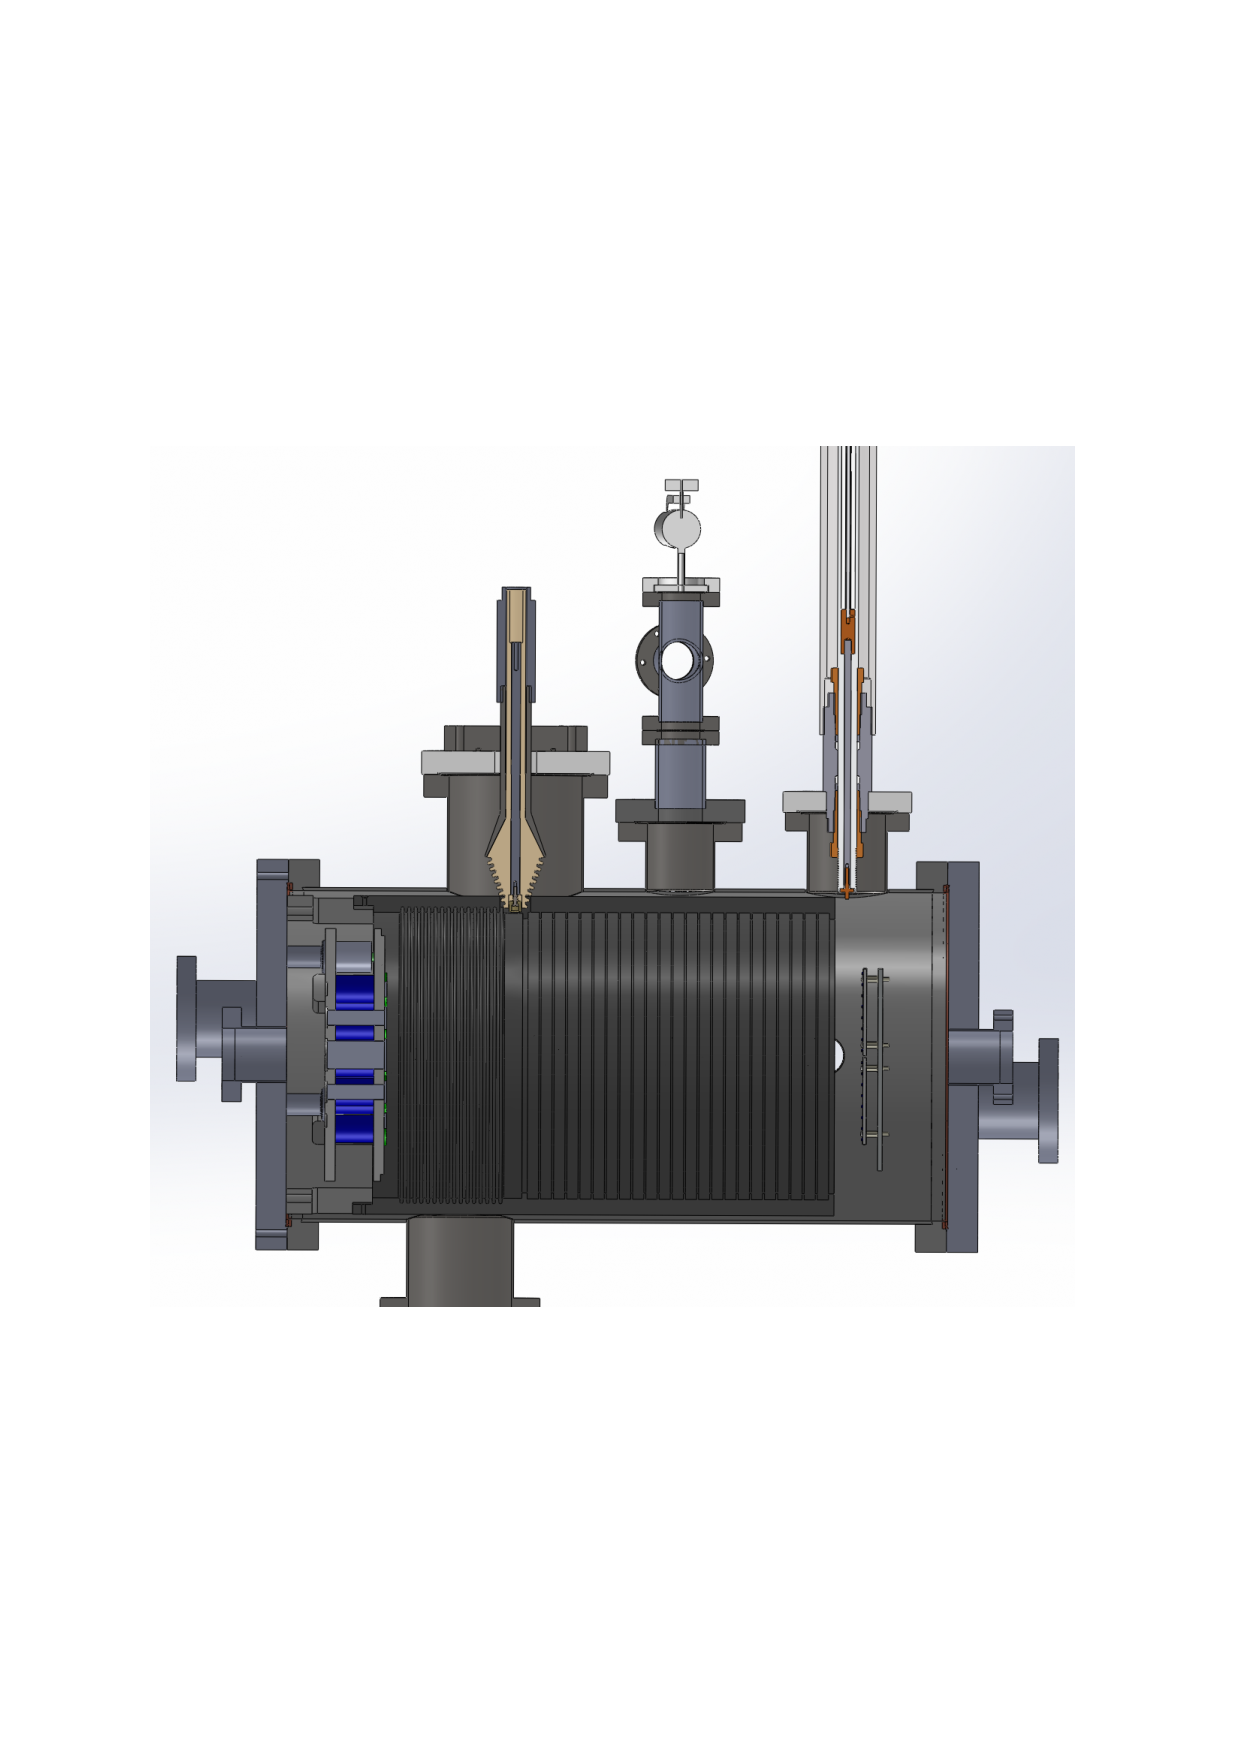
\includegraphics[width=0.45\textwidth]{img/demotest}
%\caption{Design of the test to be performed in the NEXT-DEMO detector. In the cathode (left) the feedthrough with the NEW design is used, in the gate (right) the feedthrough currently being used in DEMO is shown as reference.} \label{fig:bufftest}
%\end{figure}


\subsection{High voltage feedthroughs}

In order to create the different field regions high voltage has to be applied in different parts of the detector. Due to the impossibility of generating the high voltage (HHV) inside the detector (due radioactivity and space problems), the HHV has to be produced outside and then passed inside using feedthroughs that passes the voltage but stops gas leaks.

When discussing about feedthroughs we should differentiate three parts: The high voltage modules, the cable and the feedthrough itself.

Figure \ref{fig:hvft1}) shows the design and the results of the electric field simulations.

\begin{figure}[h!]
\centering
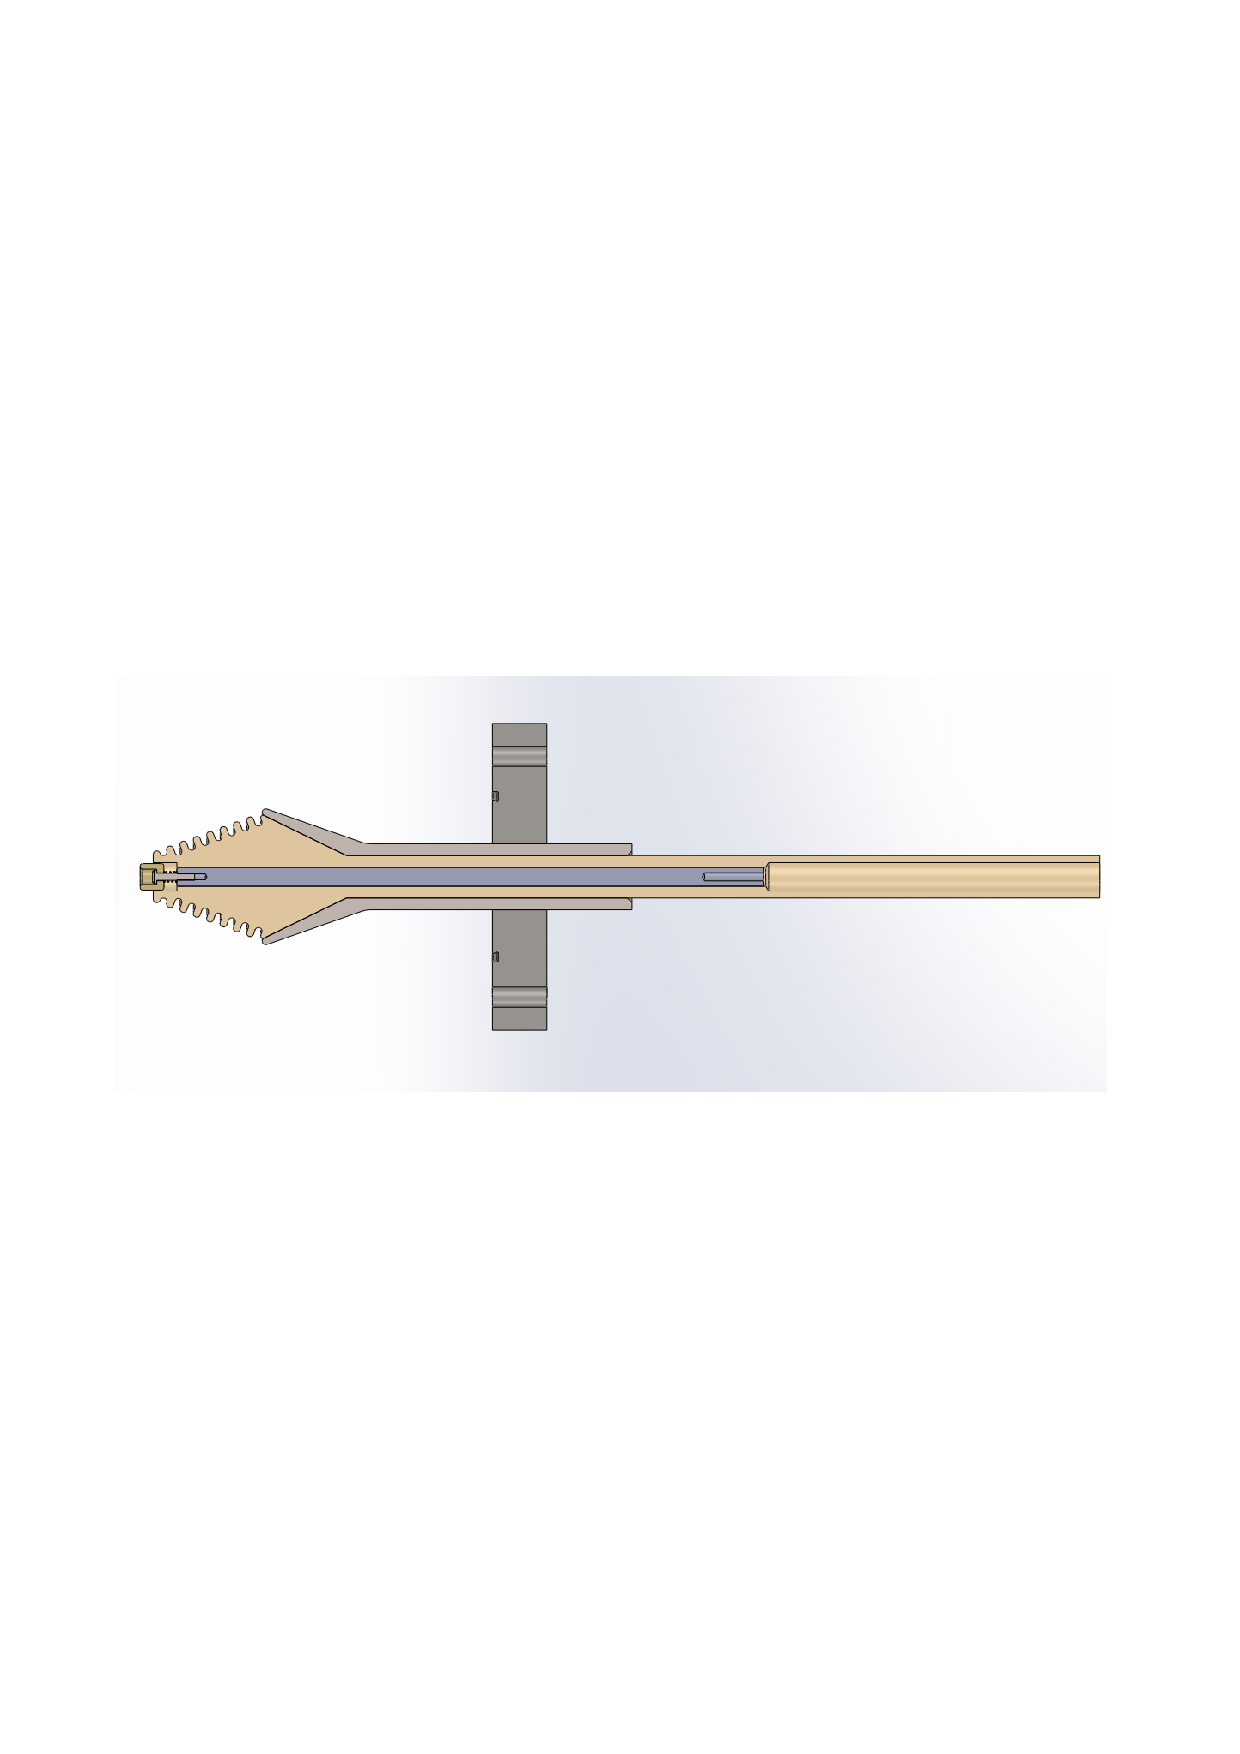
\includegraphics[width=0.45\textwidth]{img/hvft1.pdf}
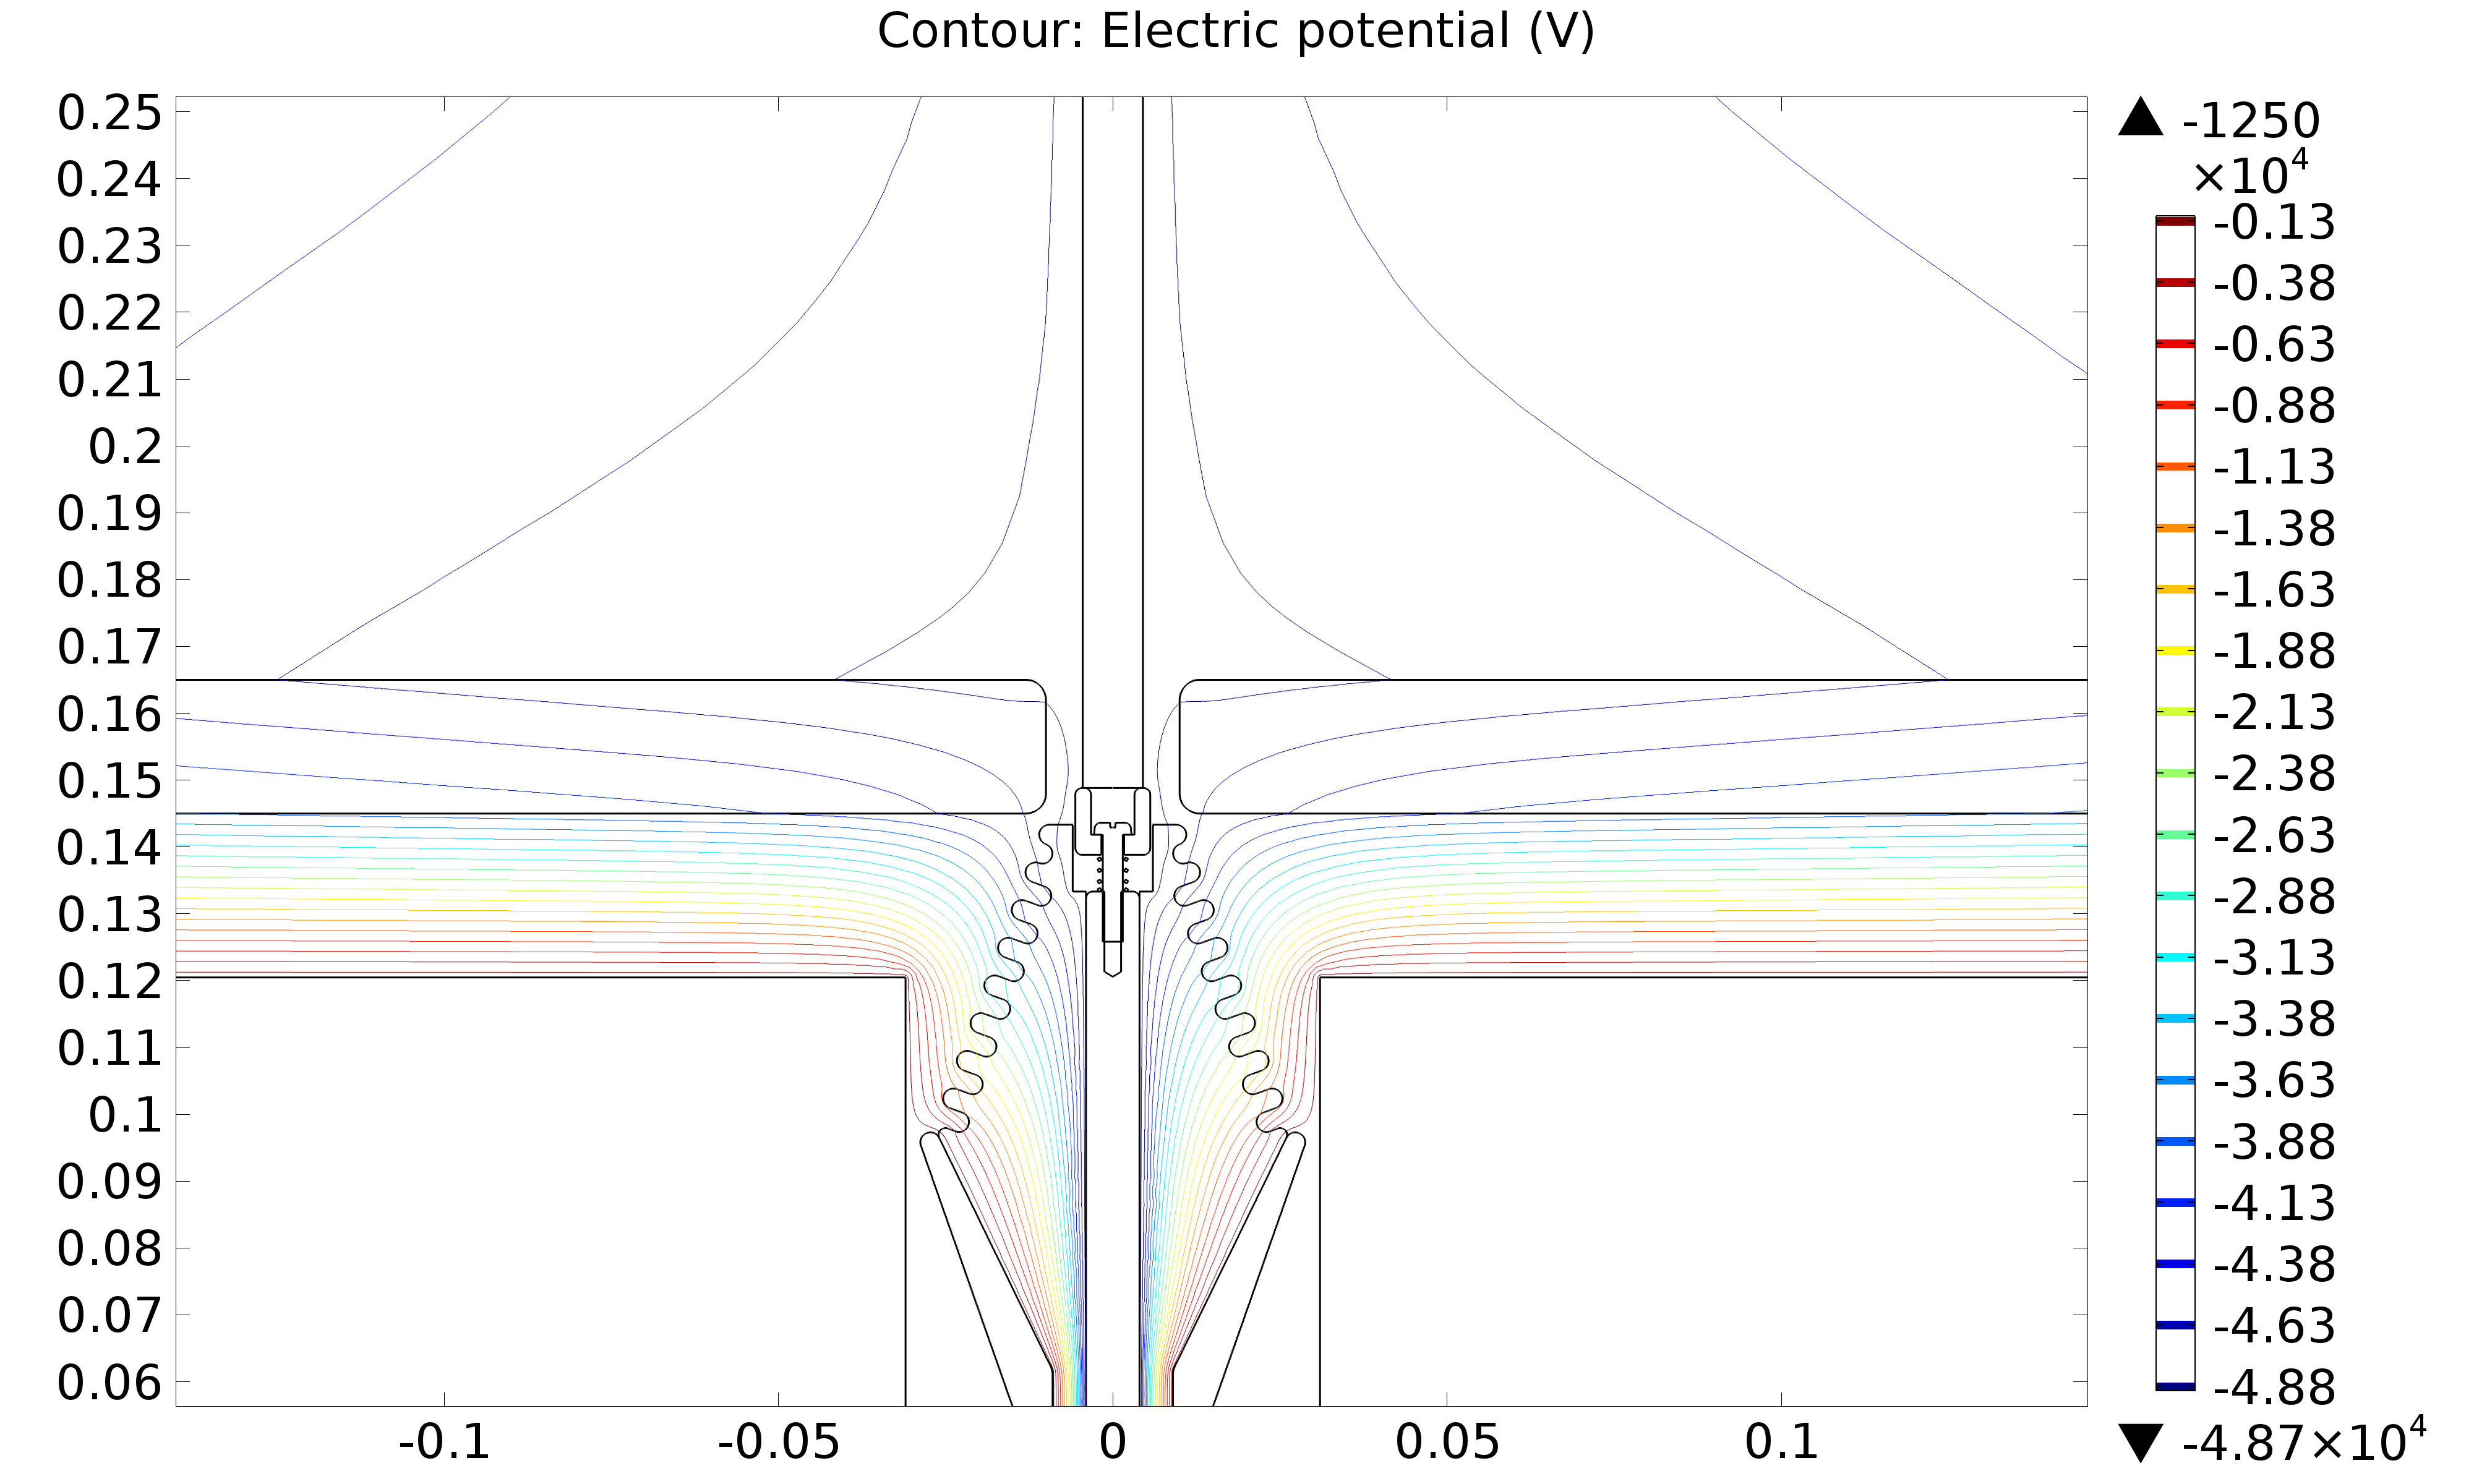
\includegraphics[width=0.45\textwidth]{img/HVFT_with_drift.png}
\caption{Design (left) and Comsol simulation (right) of the HVFT to be used in NEXT-DEMO.} \label{fig:hvft1}
\end{figure}

A key part on that design was the cryo-fitting components to create gas tight seals as all different parts of the HVFT are sealed using this technique.

%\begin{figure}[h!]
%\centering
%\includegraphics[width=0.45\textwidth]{img/cryofit1.jpg}
%\includegraphics[width=0.45\textwidth]{img/cryofit2.jpg}
%\caption{Test for the cryofit sealing. Left image shows the position of the HDPE against the outer vessel. Right image shows the inner steel conductor that will seal agains the inner hole of the HDPE.} \label{fig:hvft2}
%\end{figure}

%During assebly the feedthroughs will be separated from the main vessel and that can represent a safety issue. In order to avoid any possible damage to the people involved in the assembly the next protocol must be followed:
%
%\begin{itemize}
%\item The high voltage feedthrough (HHVFT) has to be completely disconnected from the HHV modules when putting them in place.
%\item Once they have been put in its place in the detector they can be connected to the high voltages modules.
%\item Only authorized people should be able to manipulate modules output voltage manually. Normal user should set the voltage using the slow control system as it is defined in the shifter manual.
%\end{itemize}

In the other hand, a few considerations need to be taken into account when operating the detector:

\begin{itemize}
\item The HHV modules need to be grounded using a proper connexion to the rack frame. This connexion should be check periodically to ensure the quality of the connexion.
\item The cable need to be support with a flexible/movable structure at the top  of the lead castle that will allow to hold the cable when opening/closing the castle without damaging the cable.
\end{itemize}

\subsection{Cathode grid}

The cathode grid consist of a stainless steel frame with wires to fix the potential. Figure \ref{fig:cath} show a detail of the cathode frame with the grooves for fixing the wires and the bronze tensioners.

\begin{figure}[h!]
\centering
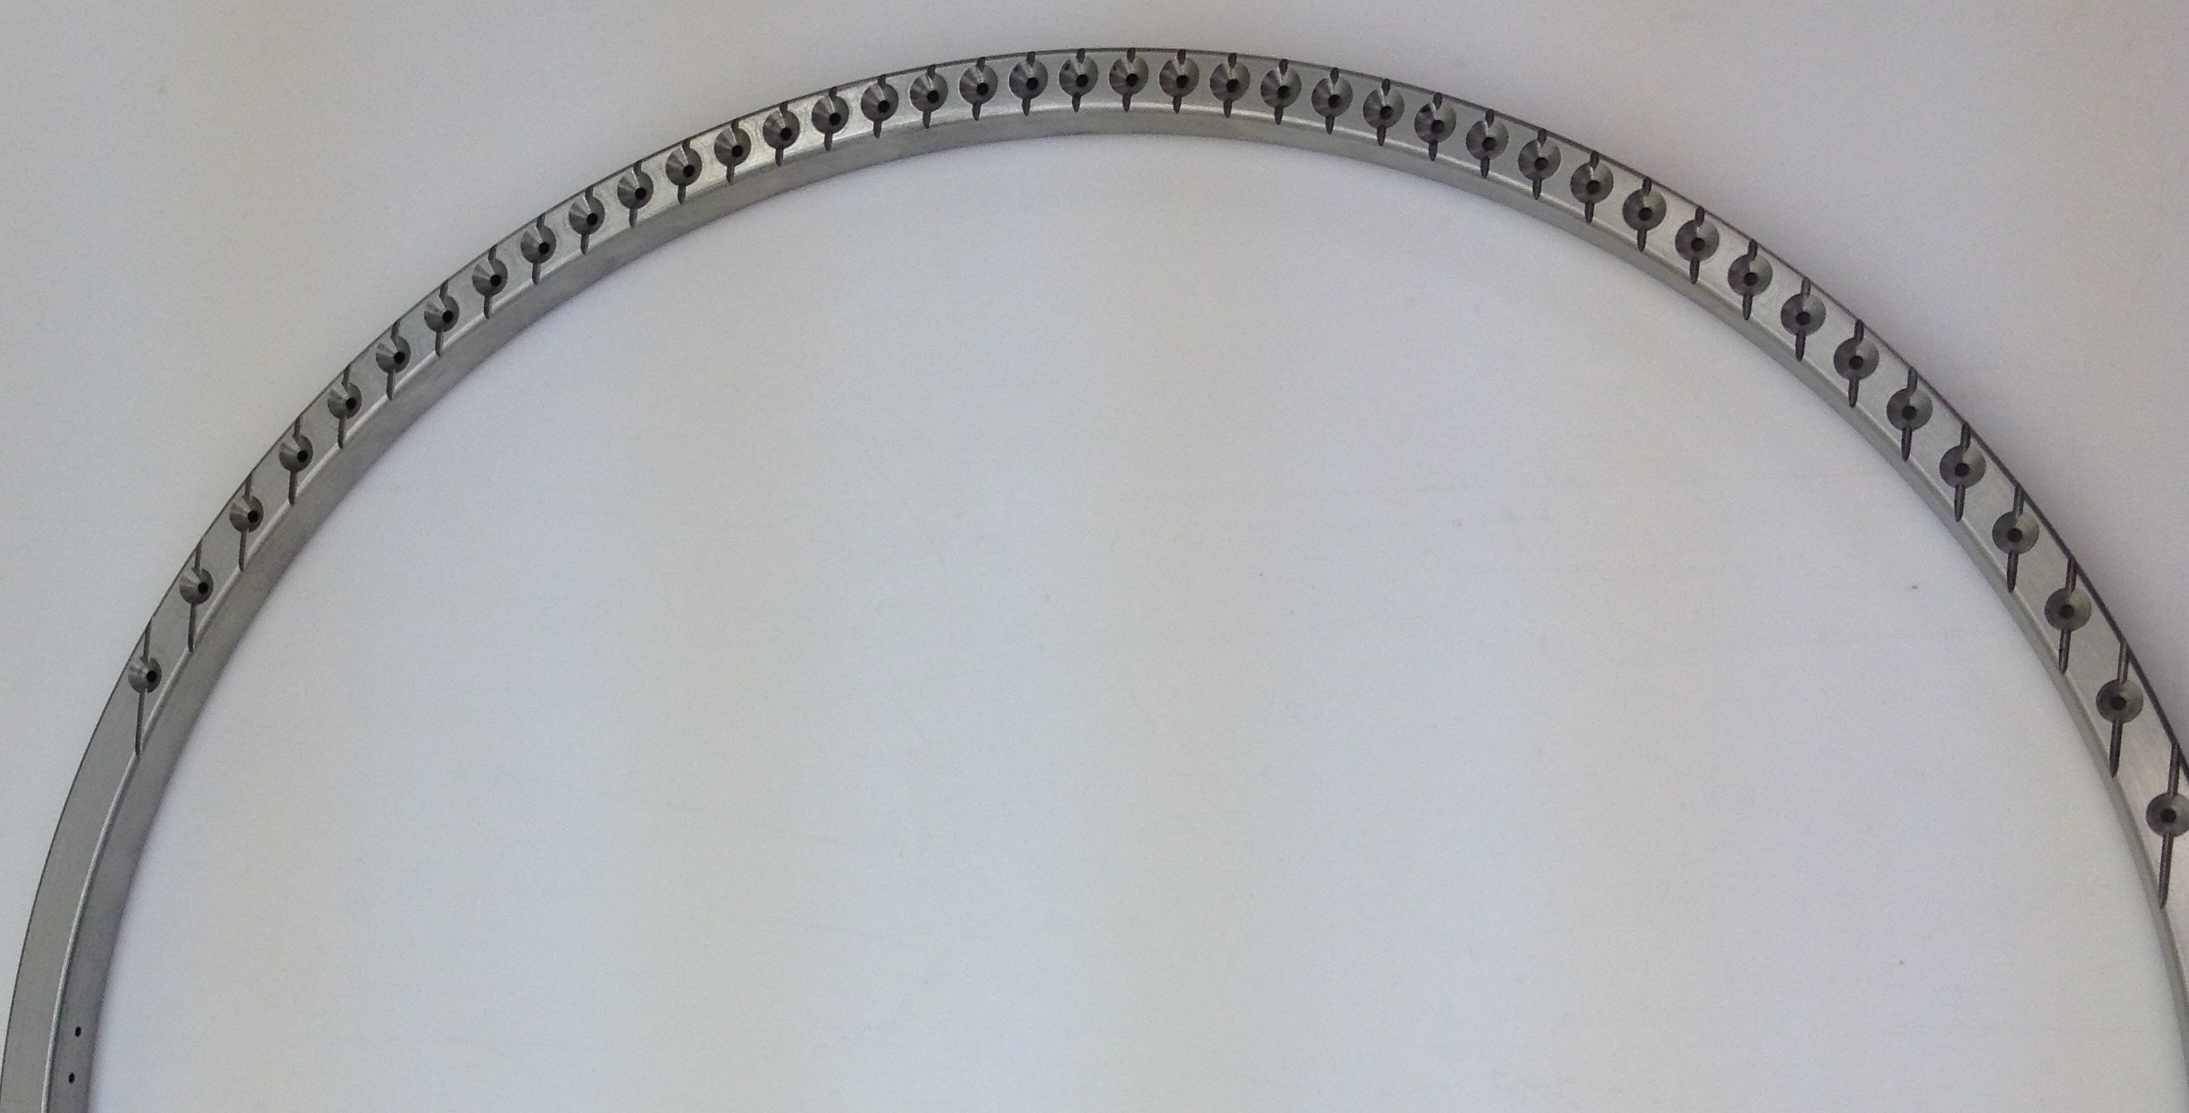
\includegraphics[width=0.45\textwidth]{img/cathode_1.jpg}
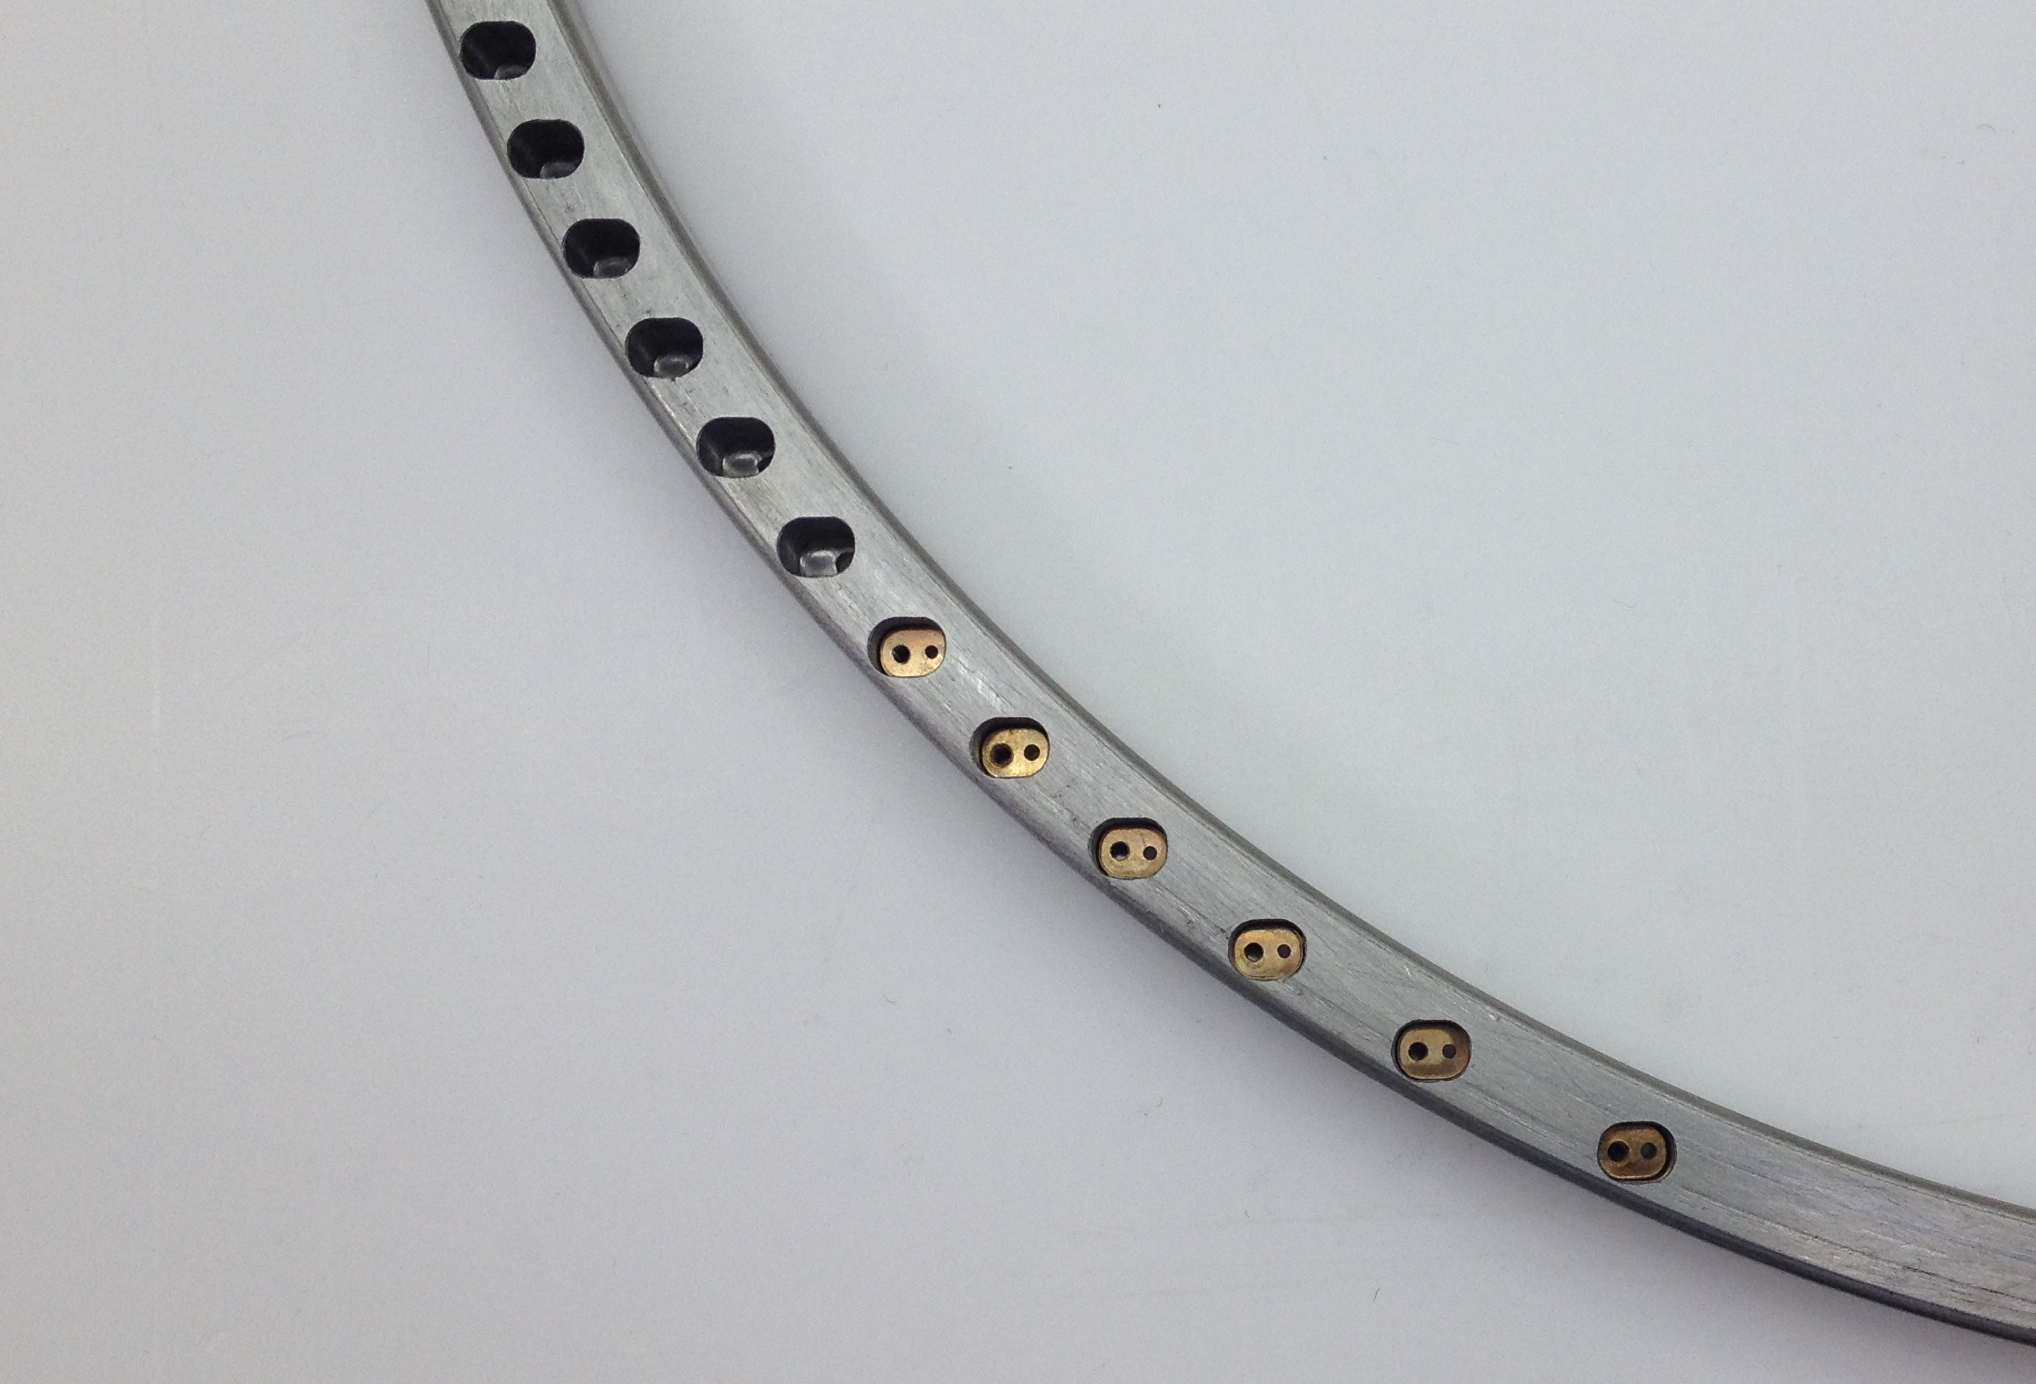
\includegraphics[width=0.45\textwidth]{img/cathode_tensioners.jpg}
\caption{Cathode frame (left) with a detail of the groves for fixing the wires. The bronze tensioners (left) will be used to strength avery wire at the right tension.} \label{fig:cath}
\end{figure}


%No safety issues have been identified with this component of the field cage.


\subsection{Electroluminescent region}

The electroluminescent region is the amplification region of the detector and it is designed to work with the highest electric field.
It consist of a steel mesh grid and a fused silica plate both supported by a HDPE frame.

The main parts of the Electroluminescent region are the mesh and the anode plate. The anode consists in a plate of fused silica coated with ITO in one side and TPB in the other. 

Figure \ref{fig:el} shows details of the different parts of the electroluminescent region.

\begin{figure}[h!]
\centering
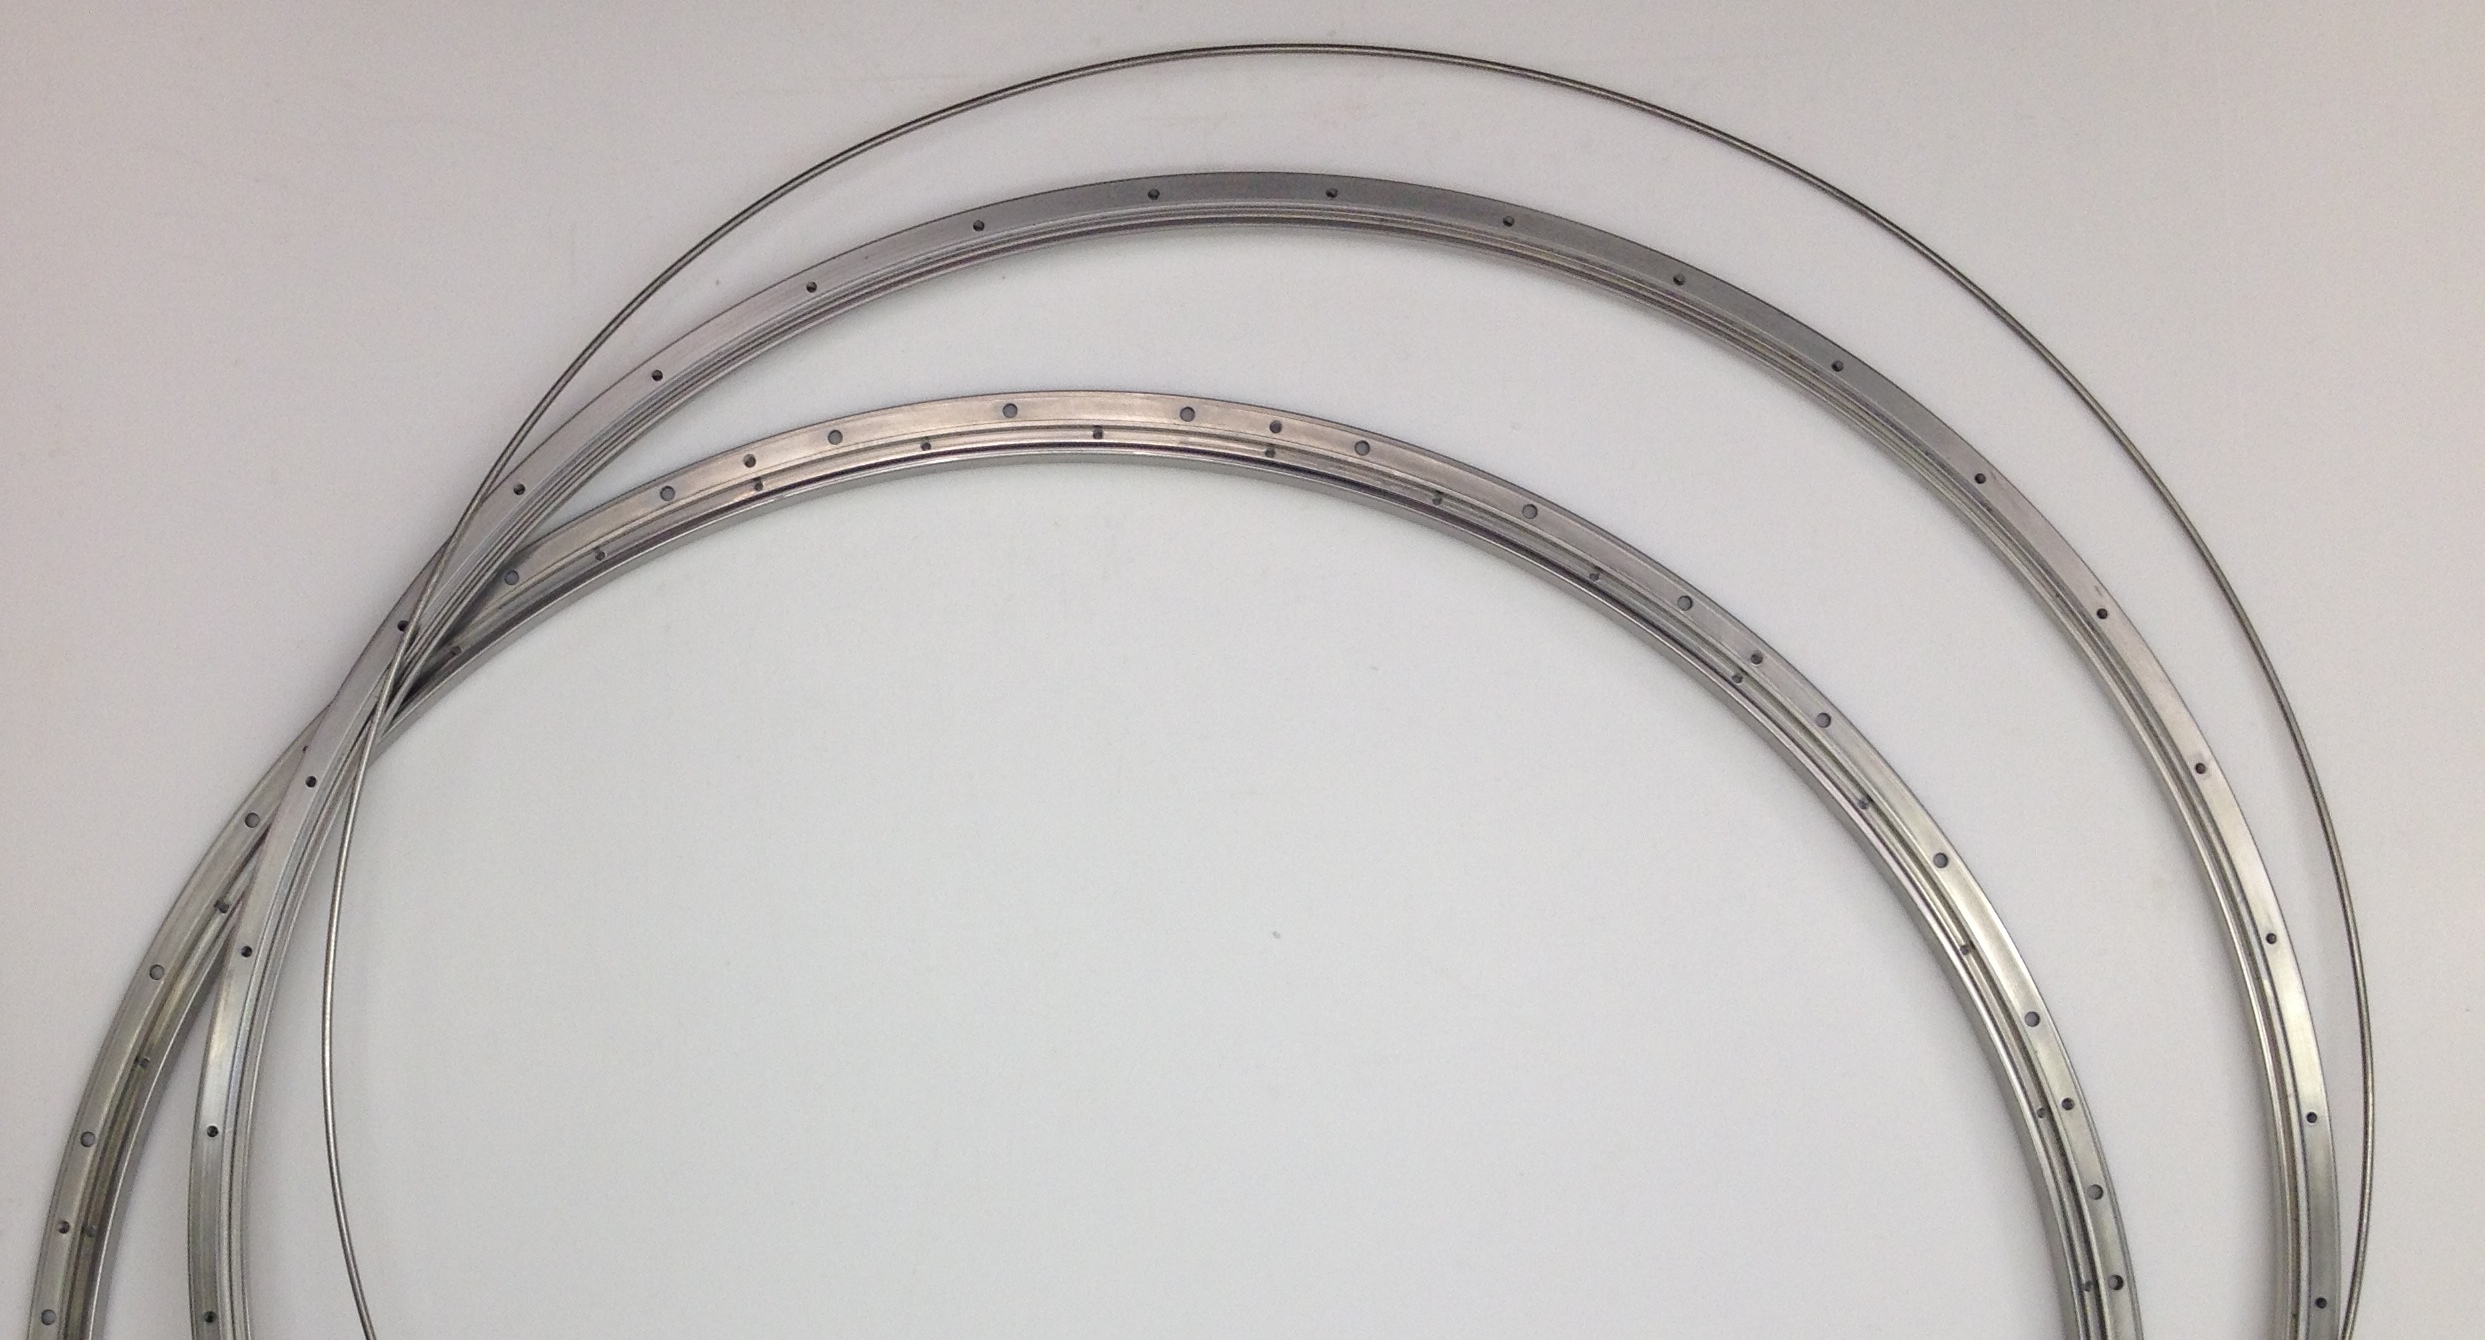
\includegraphics[width=0.45\textwidth]{img/mesh_grid_1.jpg}
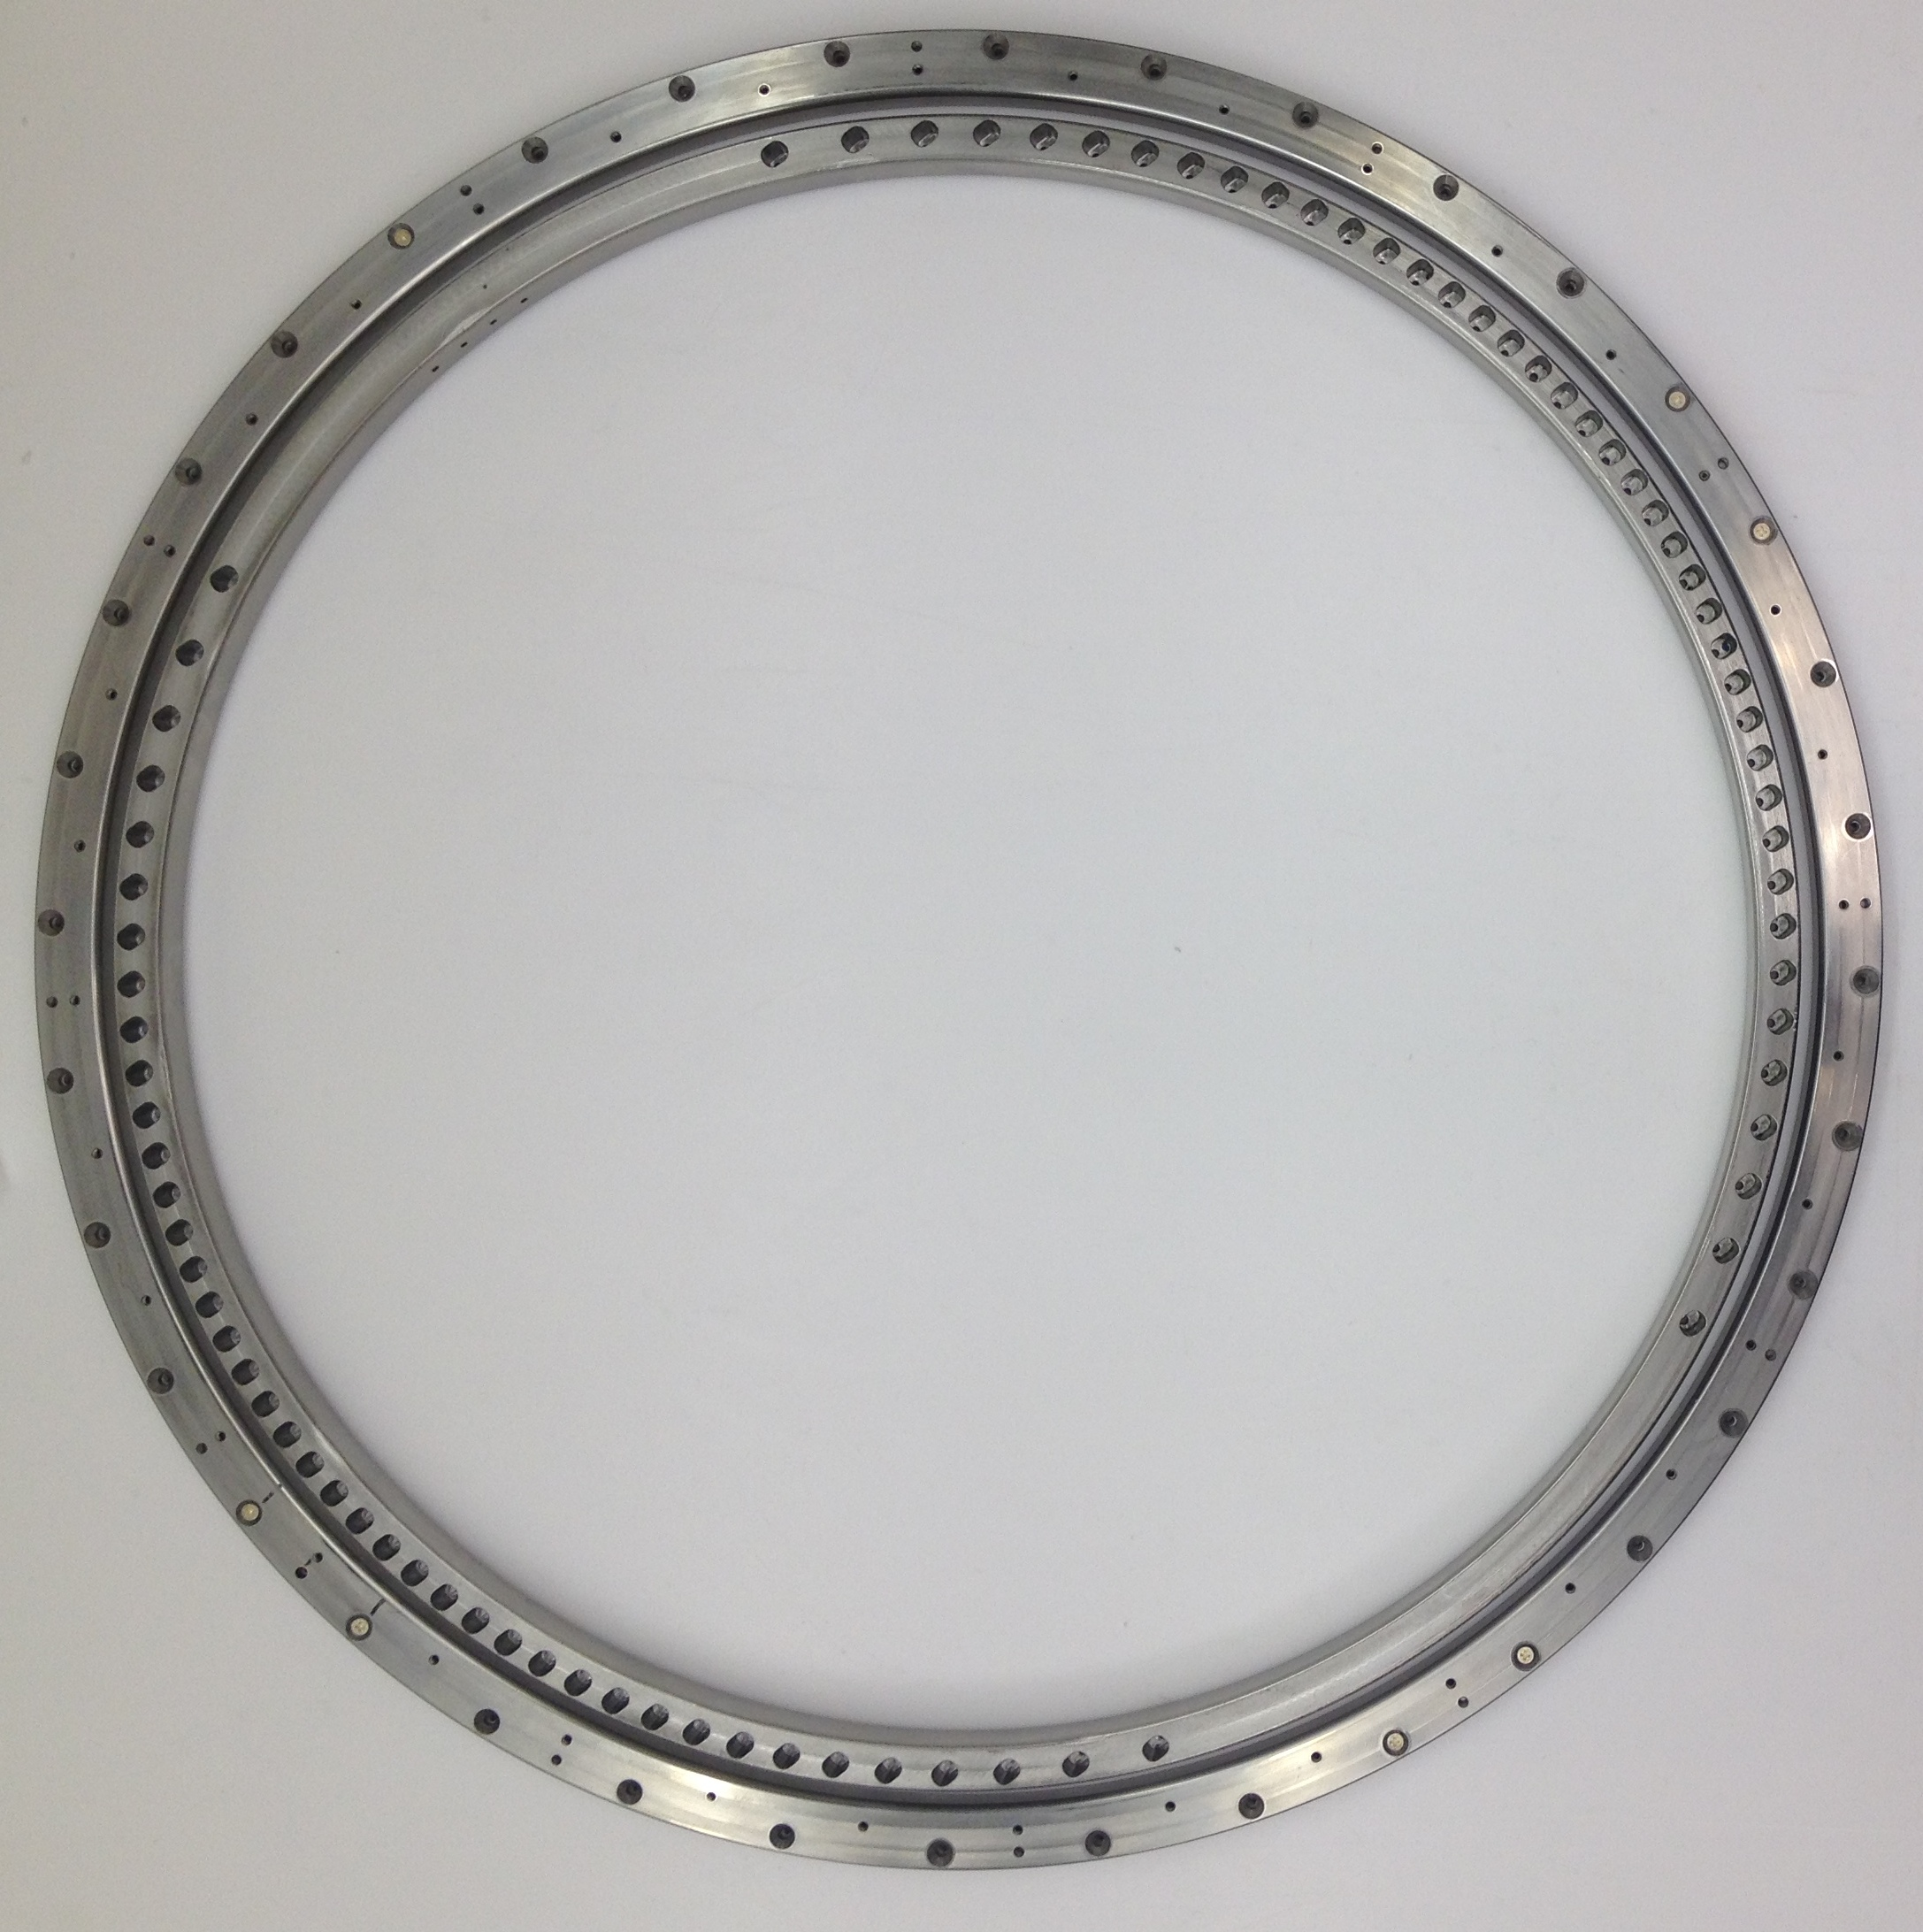
\includegraphics[width=0.45\textwidth]{img/SS_grids_1.jpg}
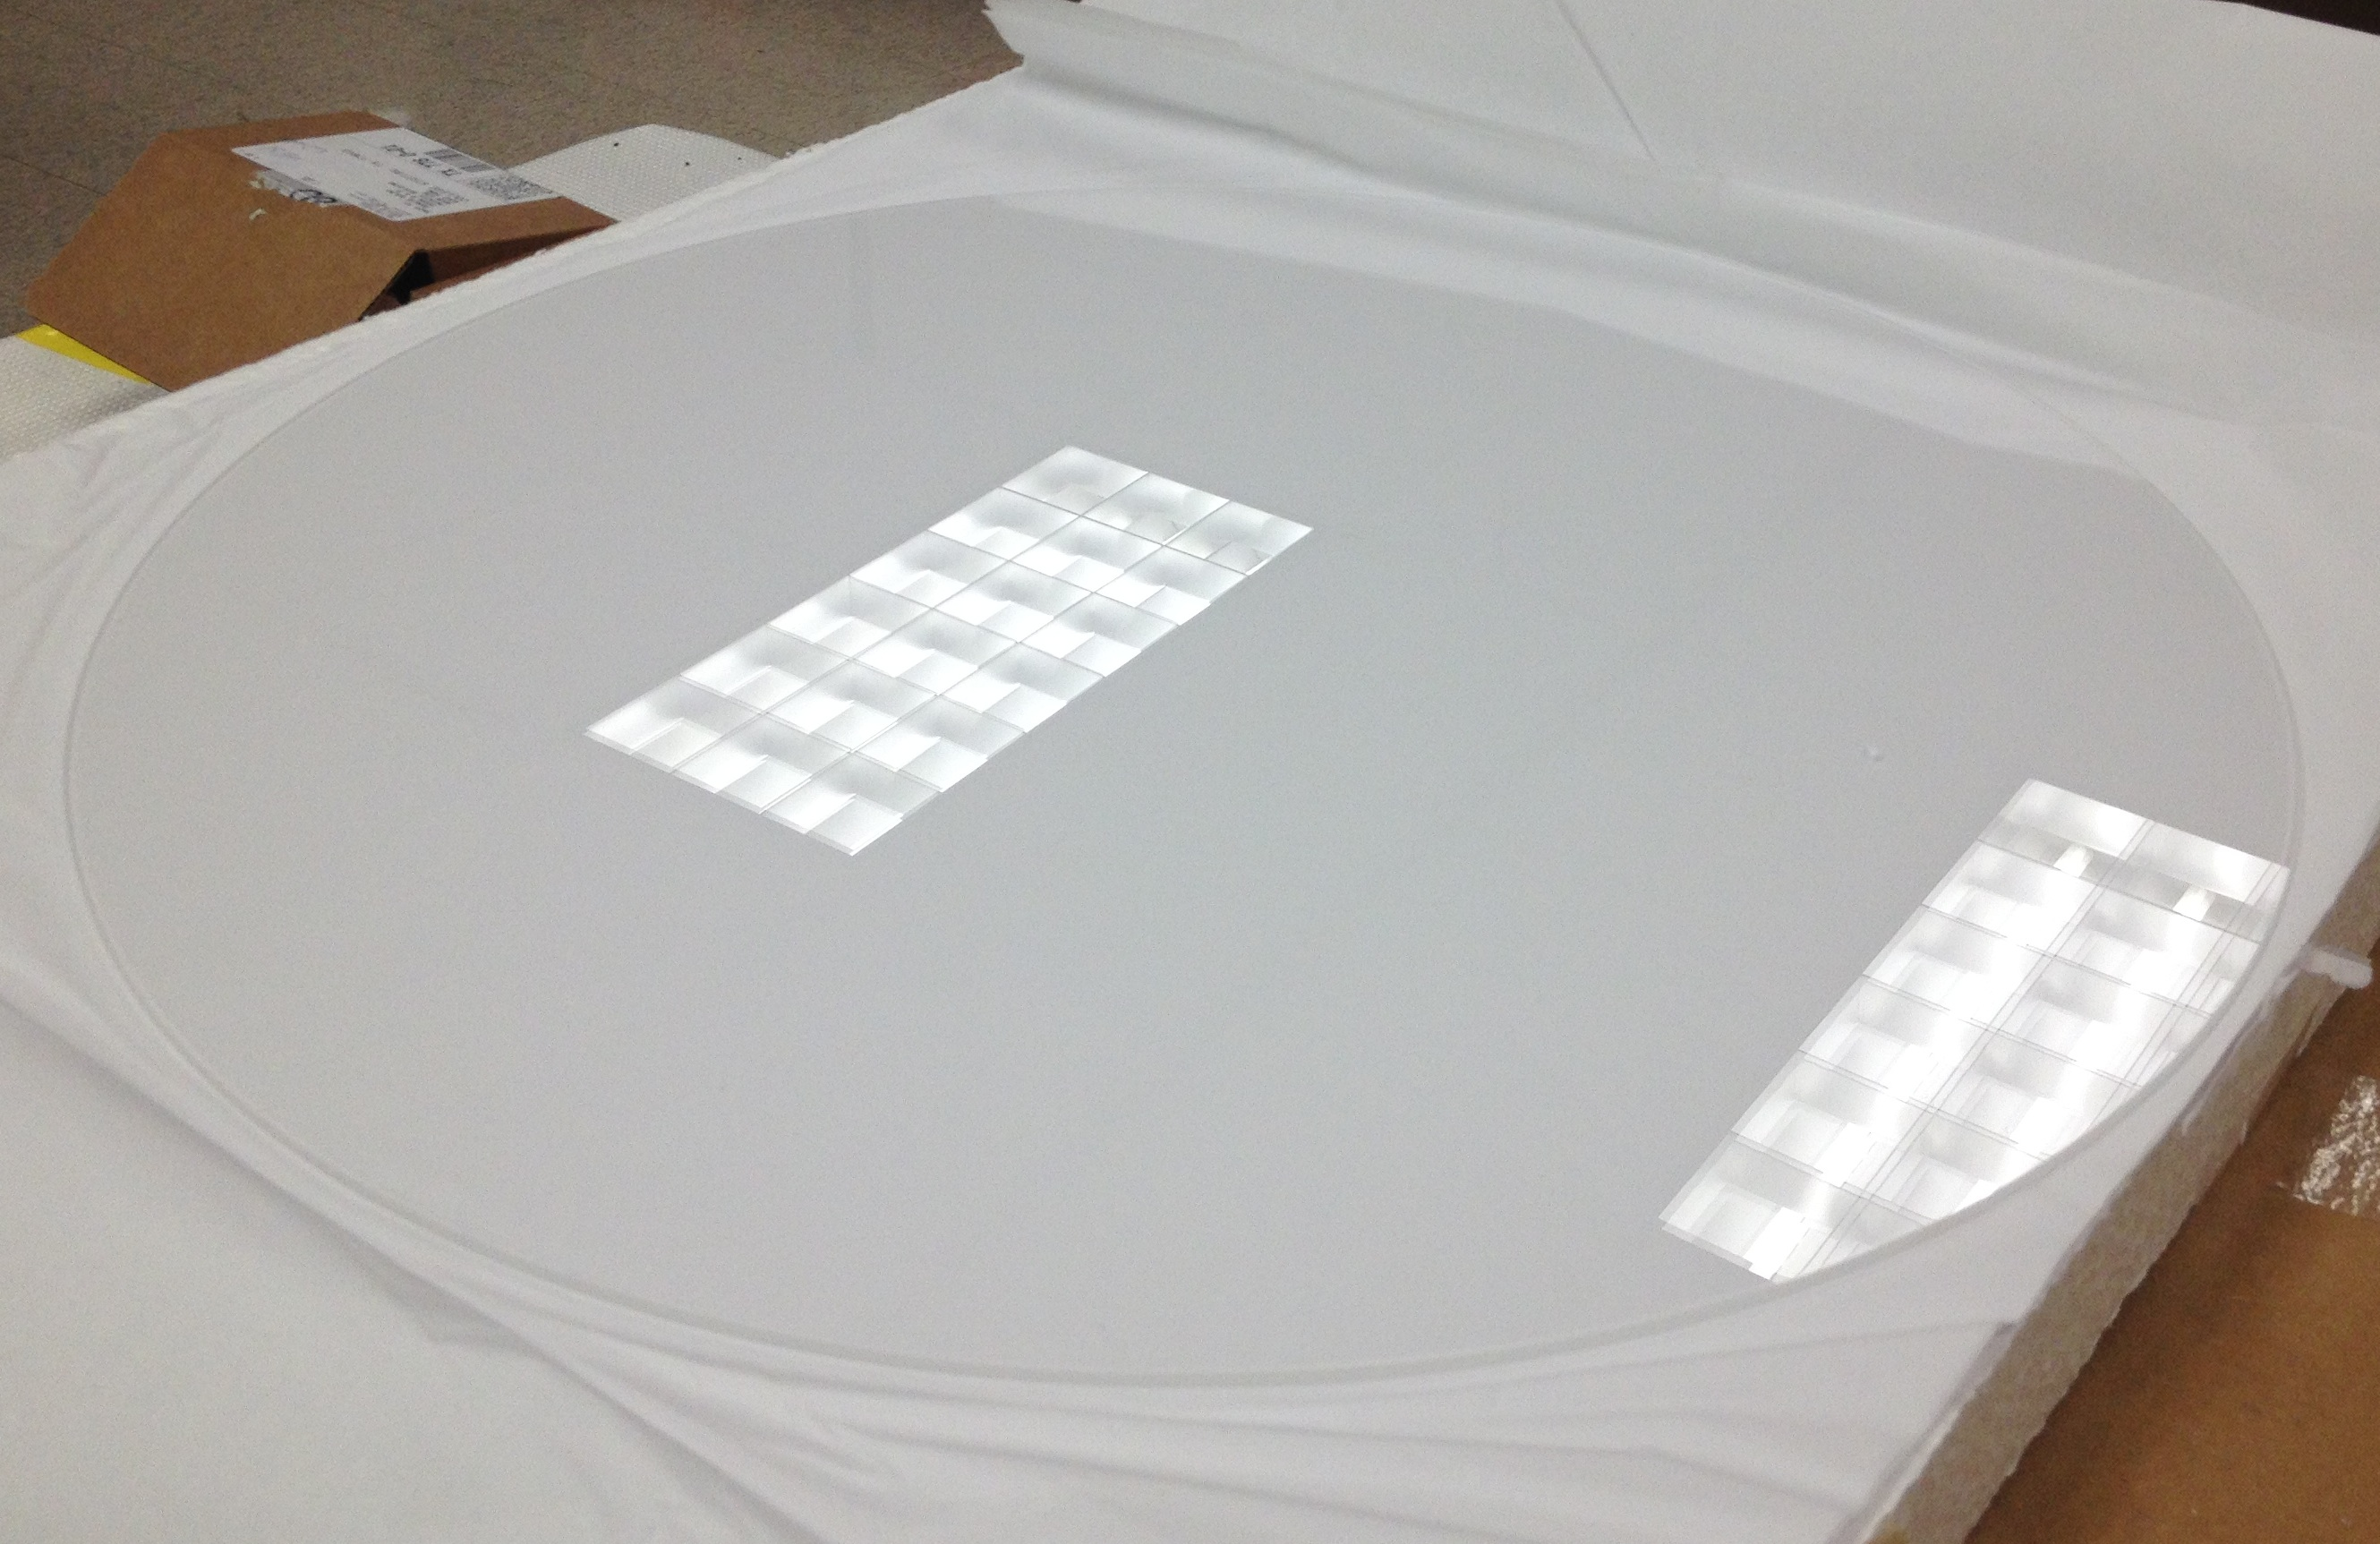
\includegraphics[width=0.45\textwidth]{img/SiO2_uncoated.jpg}
\caption{Top pictures show the diferent frames used for assembly and tension the gate mesh. Bottom is a picture of the fused silica plate before coating with ITO} \label{fig:el}
\end{figure}





%Due to the intensity of the electric field sparks may occur while operating the detector but they will happen inside the detector and so they do not represent a safety issue.

%When installing the detector the fused silica plate needs to be treated very carefull. Only people authorized by the experiment may be allow to do that.


%\section{Installation, schedule, and possible bottle necks}
%
%The time planning for  the NEW field cage ready is illustrated in Fig. \ref{fig:gantt}. It shows that the field cage could be ready by the end of July. 
%In the other hand, there exist a possible bottleneck related with the test in NEXT-DEMO. If that test fails the design of the buffer, HVFT or both will need to be redesigned and tested again. That will imply a general delay of at least one to two months in the delivery.
%
%\begin{figure}[h!]
%\centering
%\includegraphics[width=0.99\textwidth]{img/ganttchart.pdf}
%\caption{Planning to have the NEW field cage ready.} \label{fig:gantt}
%\end{figure}
%
%


\section{Electrical Power}
\label{sec:ElecPow}
The major part of the electrical power needed for the operation of NEXT-DEMO detector is related with the recirculation pump. The other components of the gas system will only require a fraction of that power. Table \ref{tab:gasPow} reflects the power consumption by the components of the gas system.


\begin{table}
\centering
\begin{tabular}{l c}
\hline
Recirculation Pump PC & 3kW\\ \hline
Roughing pump& 250 W\\\hline
Hot getter & 660 W \\ \hline \hline
\textbf{Total} & \textbf{3.91 kW}\\\hline
\end{tabular}
\caption{Power consumption for NEXT-DEMO++ gas system}
\label{tab:gasPow}
\end{table}


About the power needed for the operation of the HV and the electronics, table \ref{tab:elePow} reflects the power consumption of the different systems as the total power needed. 

\begin{table}
\centering
\begin{tabular}{l c}
\hline
DAQ PC & 5kW\\ \hline
SiPM FE Boards & 1.5kW \\ \hline
FECs & 500 W \\\hline
ATCA & 300W\\\hline
SiPMs & 30W \\\hline \hline
\textbf{Total} & \textbf{7.33 kW}\\\hline
\end{tabular}
\caption{Power consumption for NEXT-DEMO++ electronics}
\label{tab:elePow}
\end{table}

In orer to operate in a safer mode the final power request will be about 40\% more than the nominal power consumption. In that case the request will be 15.8kW.

The power supply sources used for the electronics are


\section{Experimental area distribution}

The experimental area provided for the operation of the NEXT-DEMO detector is $25m^2$, thus we have assumed a square of 5x5m. In this area we have made the best possible distribution that allow us to have everything in the room and, at the same time, give us enough clearance to move inside the room safely.

Figure \ref{fig:Distribution} shows the proposed distribution of NEXT-DEMO, the magnet, and all the different parts needed for its operation. The details of this distribution need to be discussed with CERN.

\begin{figure}
\centering
%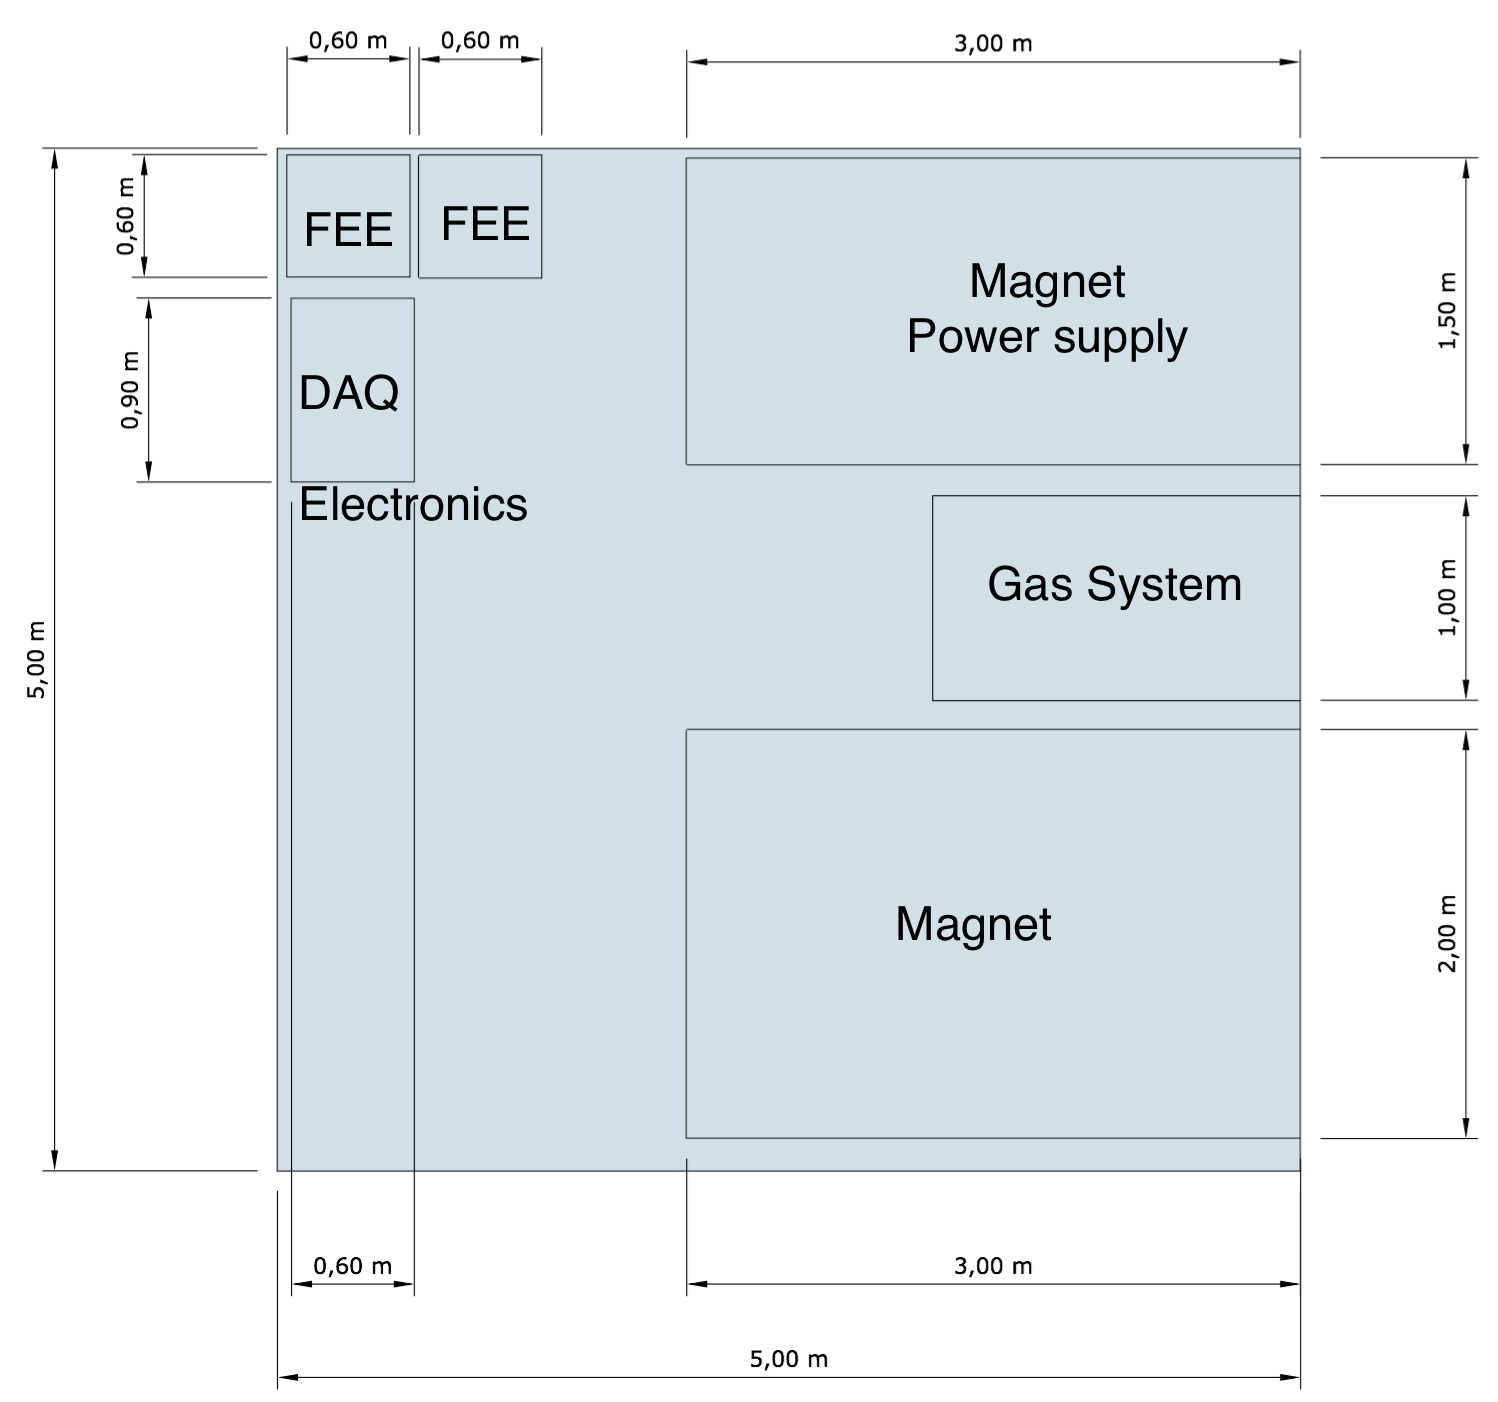
\includegraphics[width=\textwidth]{img/distribution2.png}
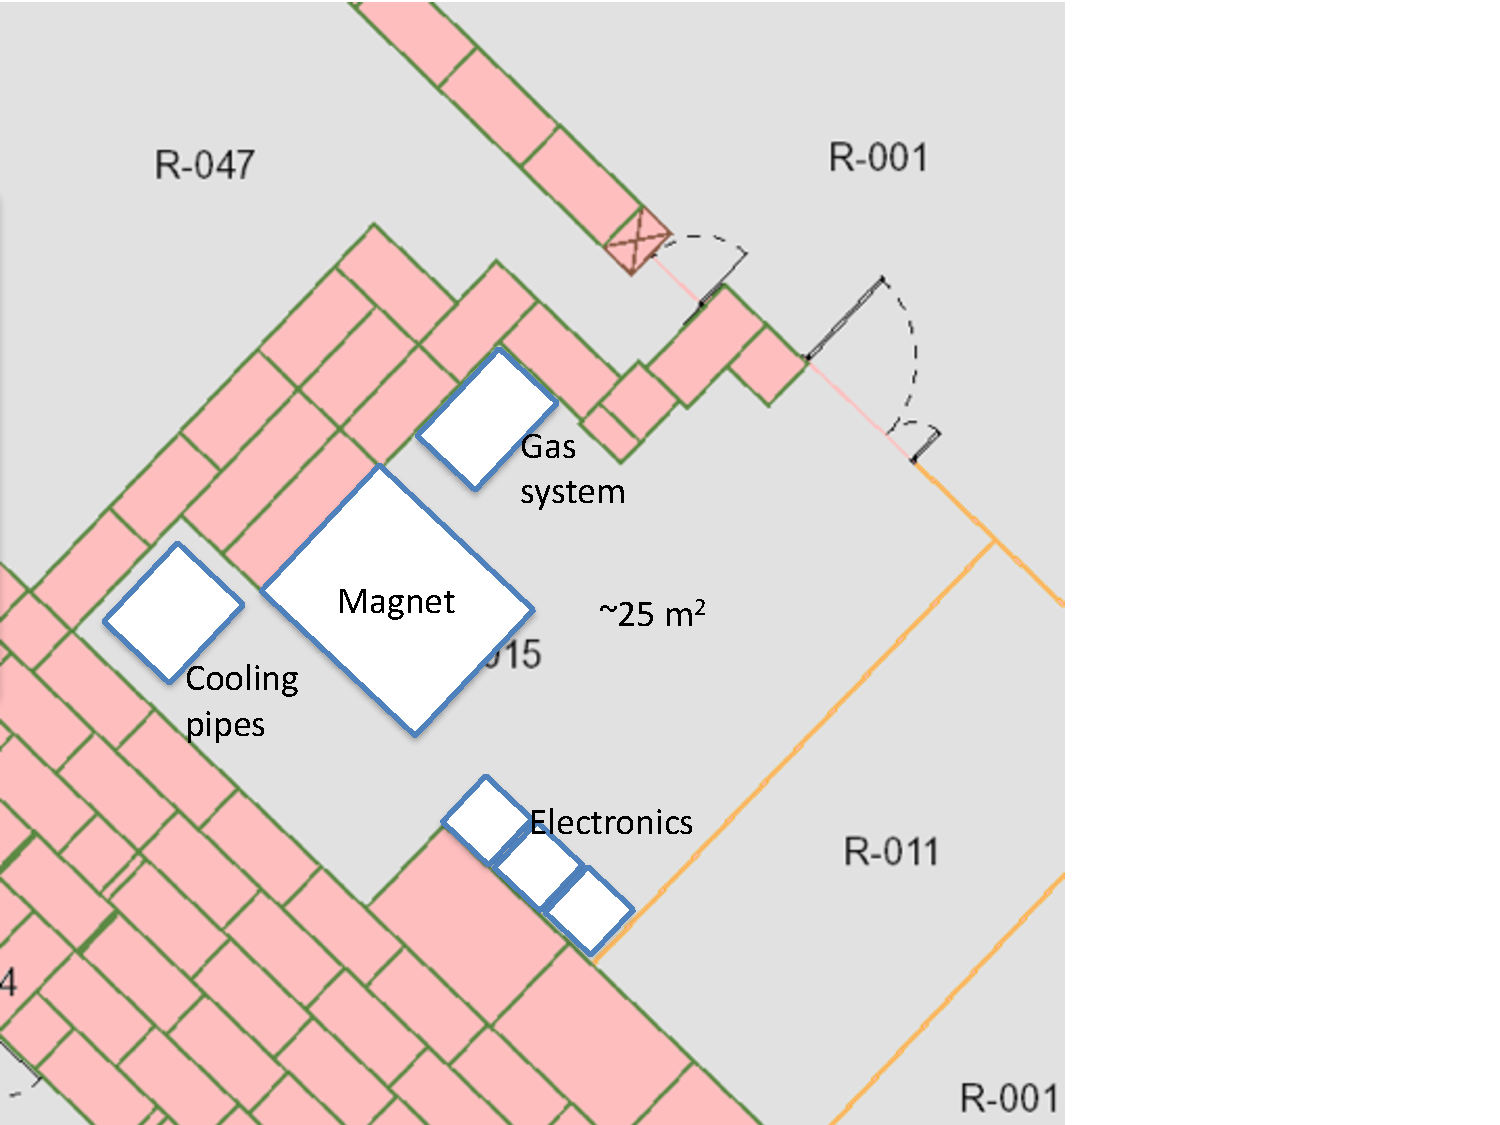
\includegraphics[angle=0,width=\textwidth]{img/distribution_examples.pdf}
\caption{Proposed distribution of the NEXT-DEMO, magnet and all different necessary systems for the operation of the detector in the experimental area} \label{fig:Distribution}
\end{figure}

The blue region will only be used for detector assembly. During detector operation and data taking this region will be free.
\section{Safety issues}

In this section we review the main issues related with safety when operating and working with the NEXT-DEMO detector evaluating the risk level for all of them. We do not include the issues related with the operation of the magnet.

\subsection{Pressure Risks}

The components that are related with pressure risks are the pressure vessel and the gas system. Both have been operating for about three years with no major problems.

\subsubsection{Pressure Vessel}
The engineering calculations and the hydrostatic test results on the vessel are attached to this document. These documents show that the operation of the NEXT-DEMO pressure vessel is safe and it doesn't represent a risk for its operation.

\subsubsection{Gas system}
The gas system is composed of standard swagelock components, all of them with the european certification for safety (CE mark). The list and scheme of the different components is shown in the correspondind attached documents. The gas system does not represent a significant risk for the operation of the NEXT-DEMO detector.

\subsubsection{Recovery Bottles}

The bottles designed for the cryogenic recovery of the Xenon from the main volume have been tested for pressure and they are safe for operation. The document of such test are included in the attahments.

\subsection{Oxygen displacement}

When operating with any gas we need to understand the effect that a total failure of the system will have on the amount of oxygen in the experimental area. The amount of Xenon used in the NEXT-DEMO detector is around 1kg, for our safety estimations we will assume 1.5kg so we are in a very pessimistic scenario.
In case of a big leak in gas system all the Xenon will be liberated into the experimental area. Operating at 10 bar and assuming a leak with a size of a 1/4" inch hole, the flow will be of the order of 0.5 $m^3/min$. The volume of 1.5kg of Xenon at 1 bar represents a volume of 8.84 cubic meters, it will take about 15 miutes to release the whole volume to the atmosphere. As Xenon is much denser than air it will stay at the bottom side. The height of the volume that Xenon will occupy is defined by the total amount of Xenon and the surface of the experimental area. As the surface of the experimental area is 25 square meters, the total height occupied by the Xenon will be 0.35 meters assuming the experimental area is sealed. That should not represent any danger for working in the area but oxygen monitors, either individual or general, are recomended to reduce this risk. Also, the slow control system switch off the pump and locks and send an e-mail giving information of a pressure drop. A light alarm can be installed in the experimental area and connected to the slow control if necessary.


%\subsection{Gas release scenarios}
%
%Even while the system has been designed to operate at pressure and it has been continuously operating at IFIC with no major problems we should contemplate different scenarios with a total release of the gas and evaluate the possible risks.
%
%\subsubsection{Normal Operation}
%During normal operation the part with a highest danger to fail is the pump diaphragm. According to the company the diphragm should be replaced avery 6 months. In our experience it is better to replace it every 4 months of continuous operation so we reduce the risk of failure.




\subsubsection{Safety systems implemented}
A slow control system has been developed in order to monitor the pressure in different parts of the gas system and pressure vessel. The slow control can start/stop the re-circulation pump and also block the system in case a leak is detected so the gas remains inside the system. The slow control represents an extra help for improving the safety.

Moreover, the gas system has two bursting disks for a controled break in case of over-preassure. One in the vacuum side for protecting the vacuum instruments (turbo molecular pump, RGA,...) and one in the pressure side that breaks at 13 bar to prevent any high over-pressure of the system.



\subsection{High Voltage safety}

The high voltage to create the electric field in TPC is generated by two High voltages modules (\textit{FUG HCP 140-100000} and \textit{FUG HCP 0-35000)}. Those modules have a fine tunning potentiometer for both voltage and current, allowing us to limit the total power and current produced byt the module. Moreover, they can be controled remotely using an IP connexion. During normal operation the modules are always controled using a special Slow Control software developed by the IFIC grup using LabView$^{\textcopyright}$ libraries. That prevents any errors in the manipulation of the modules and also helps with fast response in case of any failure.
The documentation related with the modules can be found in the folder "HHV Power Supplies"
Moreover, there is no direct acces to the any point that is at high voltage, all of them will be either inside the detector or inside the modules. That shows that the high voltage operation does not represent a risk for the operation of the detector.


\subsection{Fire}

As the gases used in the operation of NEXT-DEMO are not flamable the only system that is affected by the risk of fire is the electronics. The total power is not very high (see section \ref{sec:ElecPow}) and the electronics has been operating for a long time without any problem, we consider that the risk of having fire in the experimental area is minimum. In case that a extinguisher system is needed we can design a system using extinguishers directly in the electronics racks that are activated using a serie of smoke detectors. In that case we will recommend powder extinguisher as they can be used in the electronics and at the same time they can not produce a problem related with air displacement like the $CO_2$ extinguishers.


\subsection{Cryogenics}

For the recovery of the Xenon to the recovery bottles the use of liquid Nitrogen is needed. The recovery bottles are in a thermally insolated container that on one hand makes the process more efficient and also prevents Nitrogen to spill in the experimental area.

When using liquid Nitrogen indivual protection such as gloves and face protection is required. 




\section{Risk assessment for the DEMO++ gas system}

This section describes the riks assessment related with the operation of the DEMO++ gas system in the proposed experimental area (R015).

\subsection{Characteristics of the area}

The location of the experimental area can be seen in Fig. \ref{fig:location}. The size and distribution of the area can be seen in \ref{fig:Distribution2}. The area has a total surface of 25$m^2$, and a general view of the area is presented in Fig. \ref{fig:pictures}.

As it can be seen in Figure \ref{fig:Distribution2} and the area's pictures (Figure \ref{fig:pictures}) three of the walls and the floor appear to be reasonably gas tight. The area is open in one side, only covered with a metallic gate. Therefore we assume that any xenon gas leak will eventually diffuse though that gate.  

\begin{figure}
\centering
%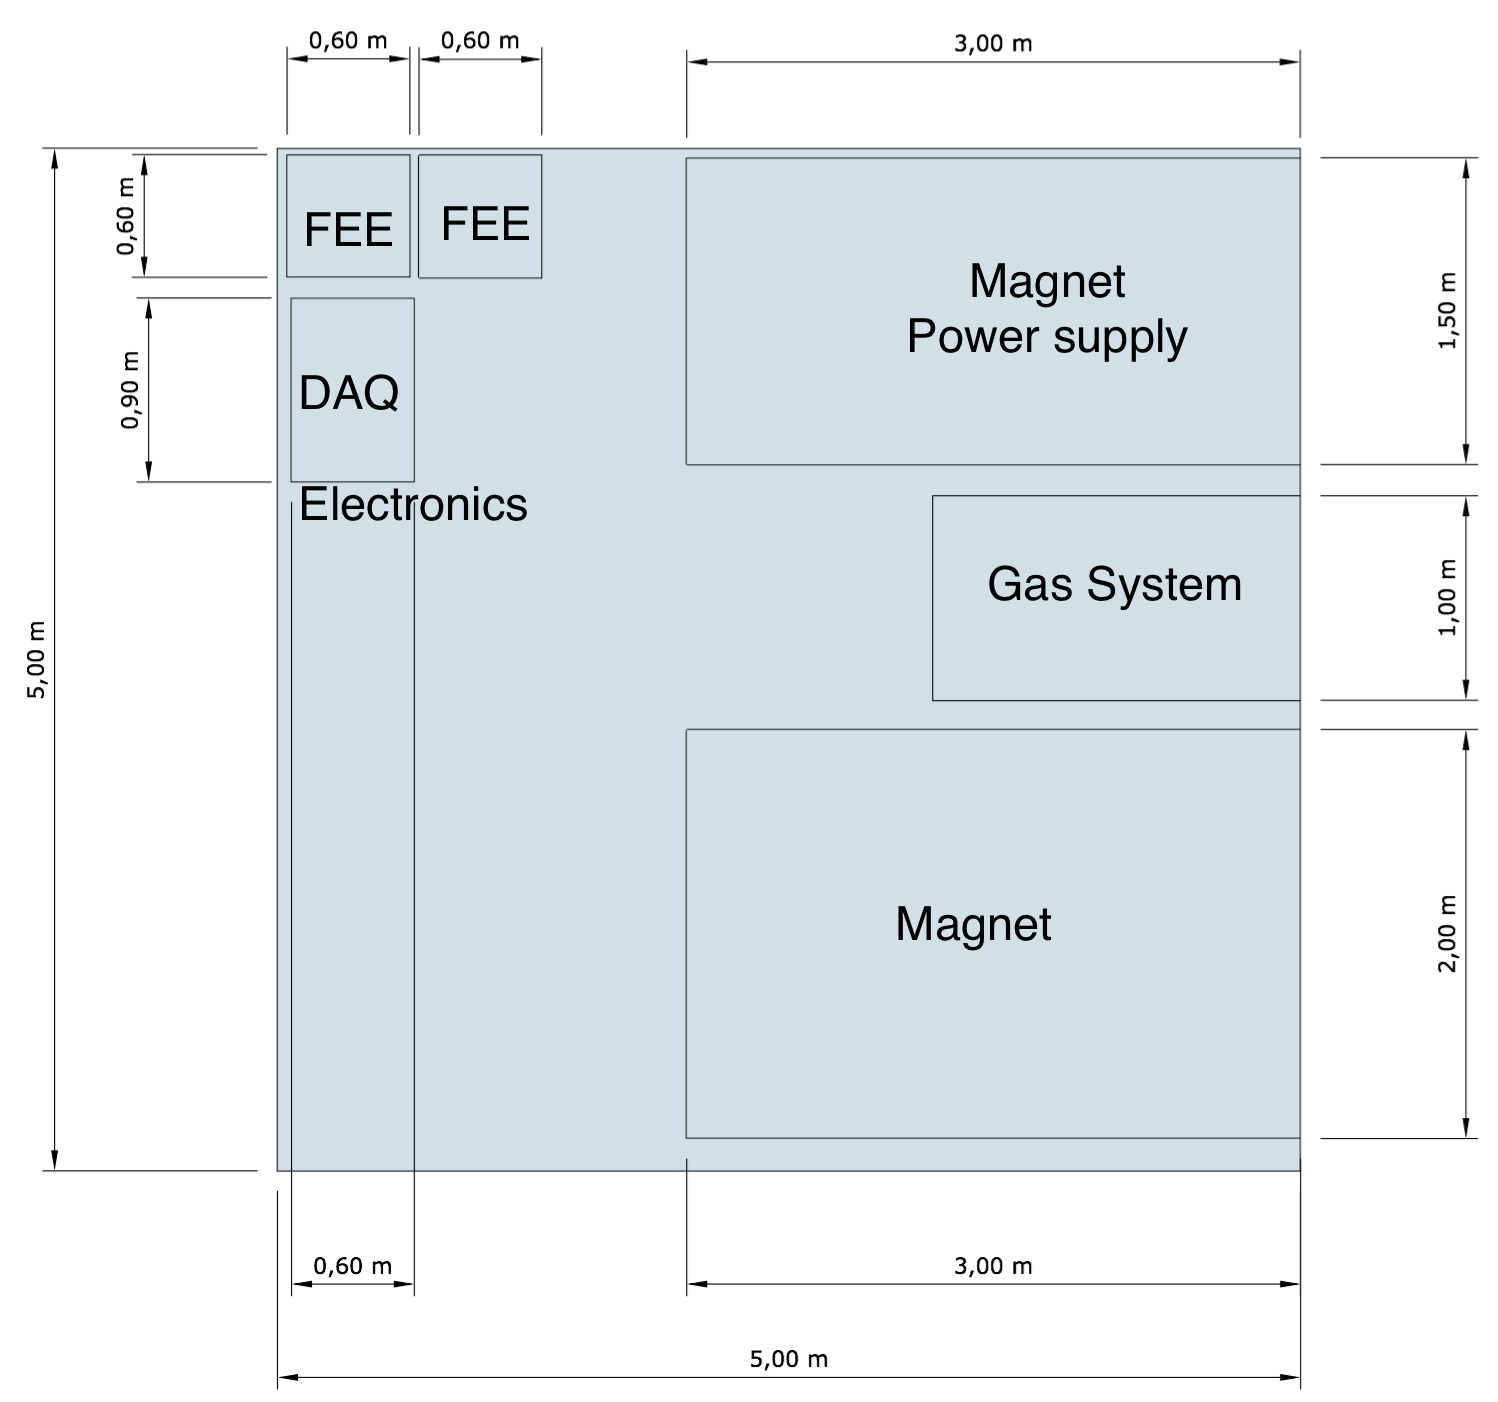
\includegraphics[width=\textwidth]{img/distribution2.png}
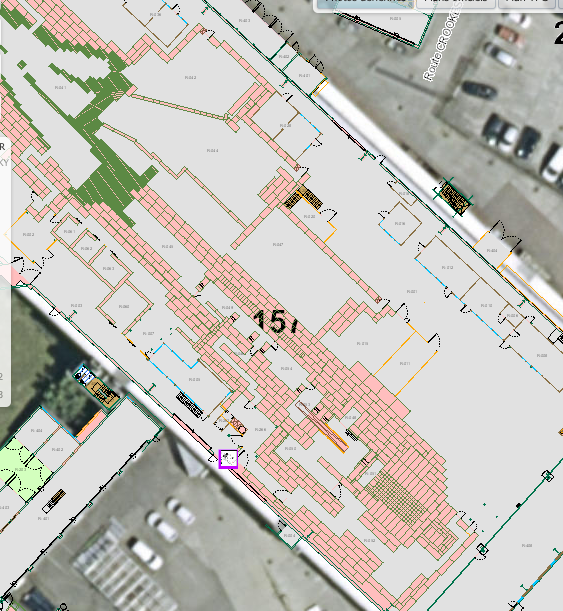
\includegraphics[angle=0,width=\textwidth]{img/generalmap.png}
\caption{Location of the experimental area} \label{fig:location}
\end{figure}


\begin{figure}
\centering
%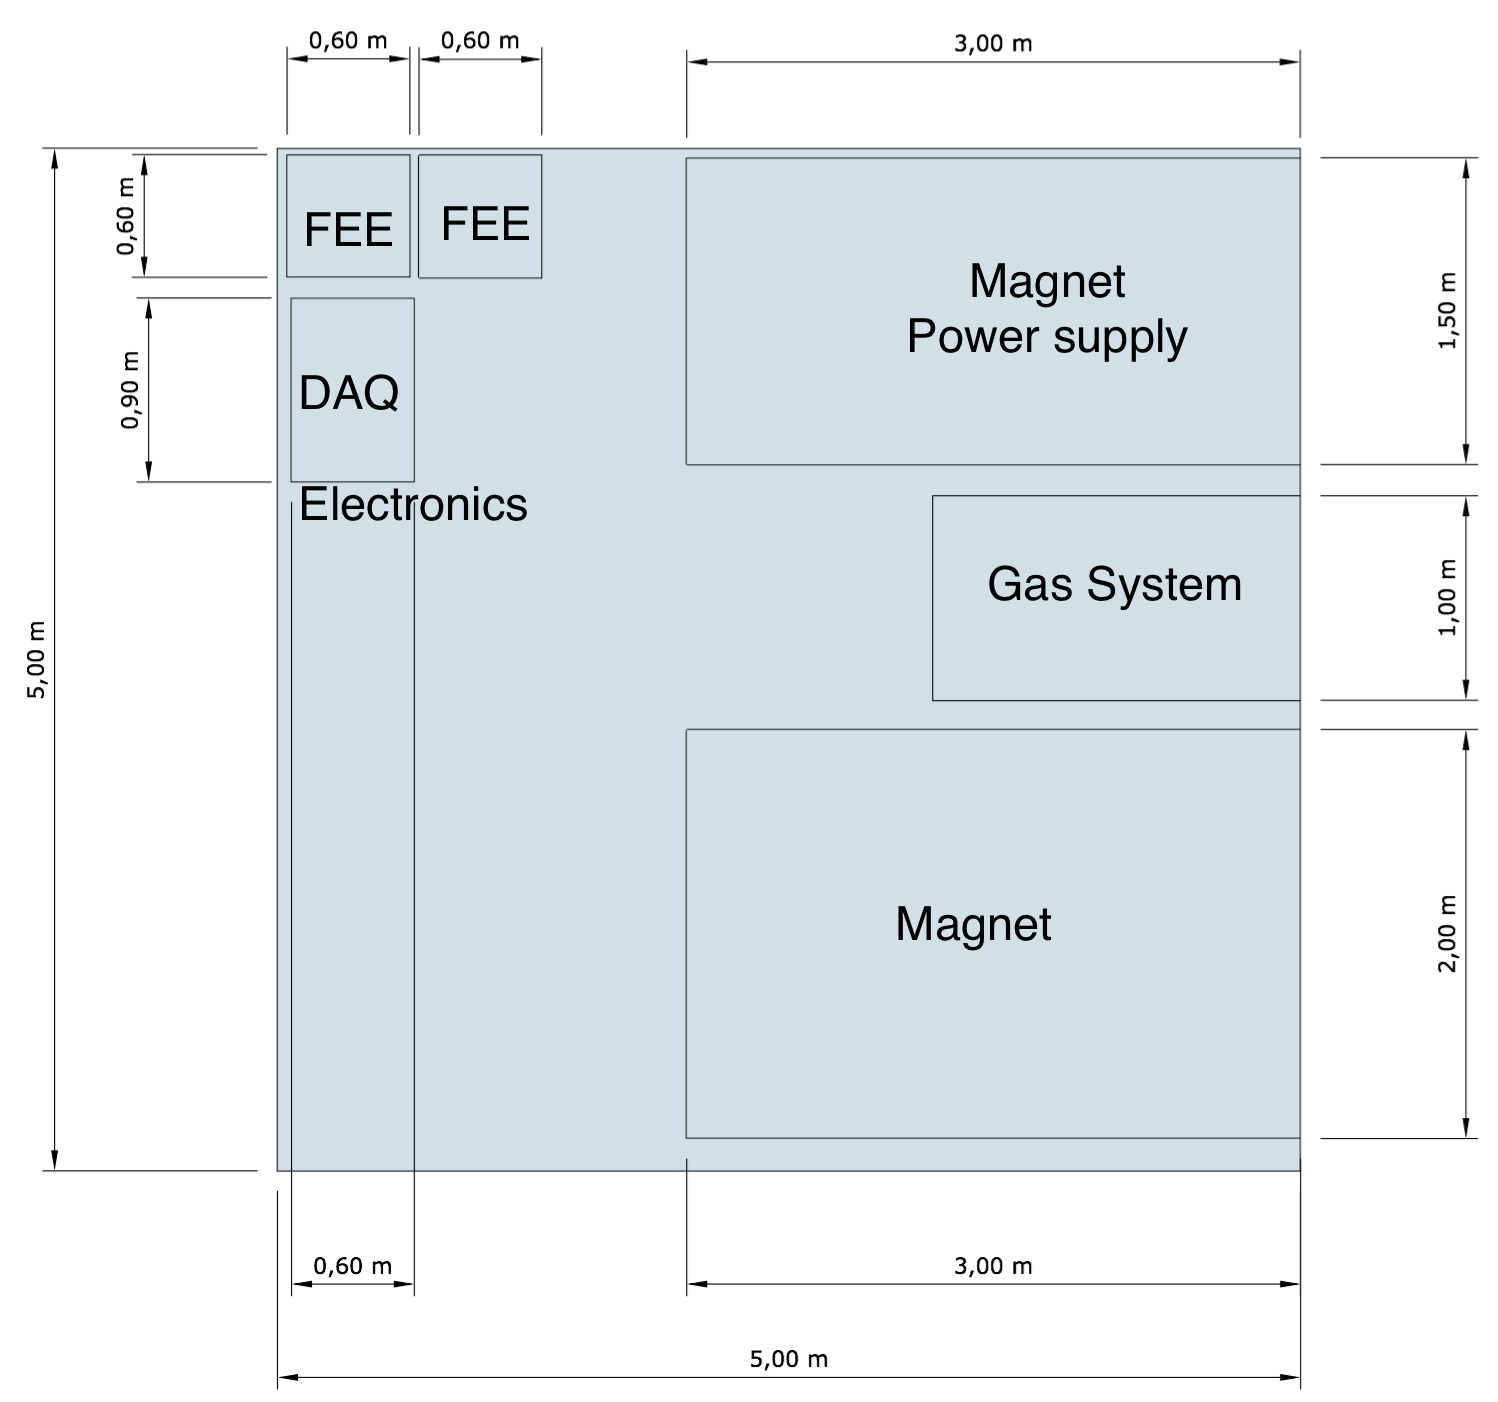
\includegraphics[width=\textwidth]{img/distribution2.png}
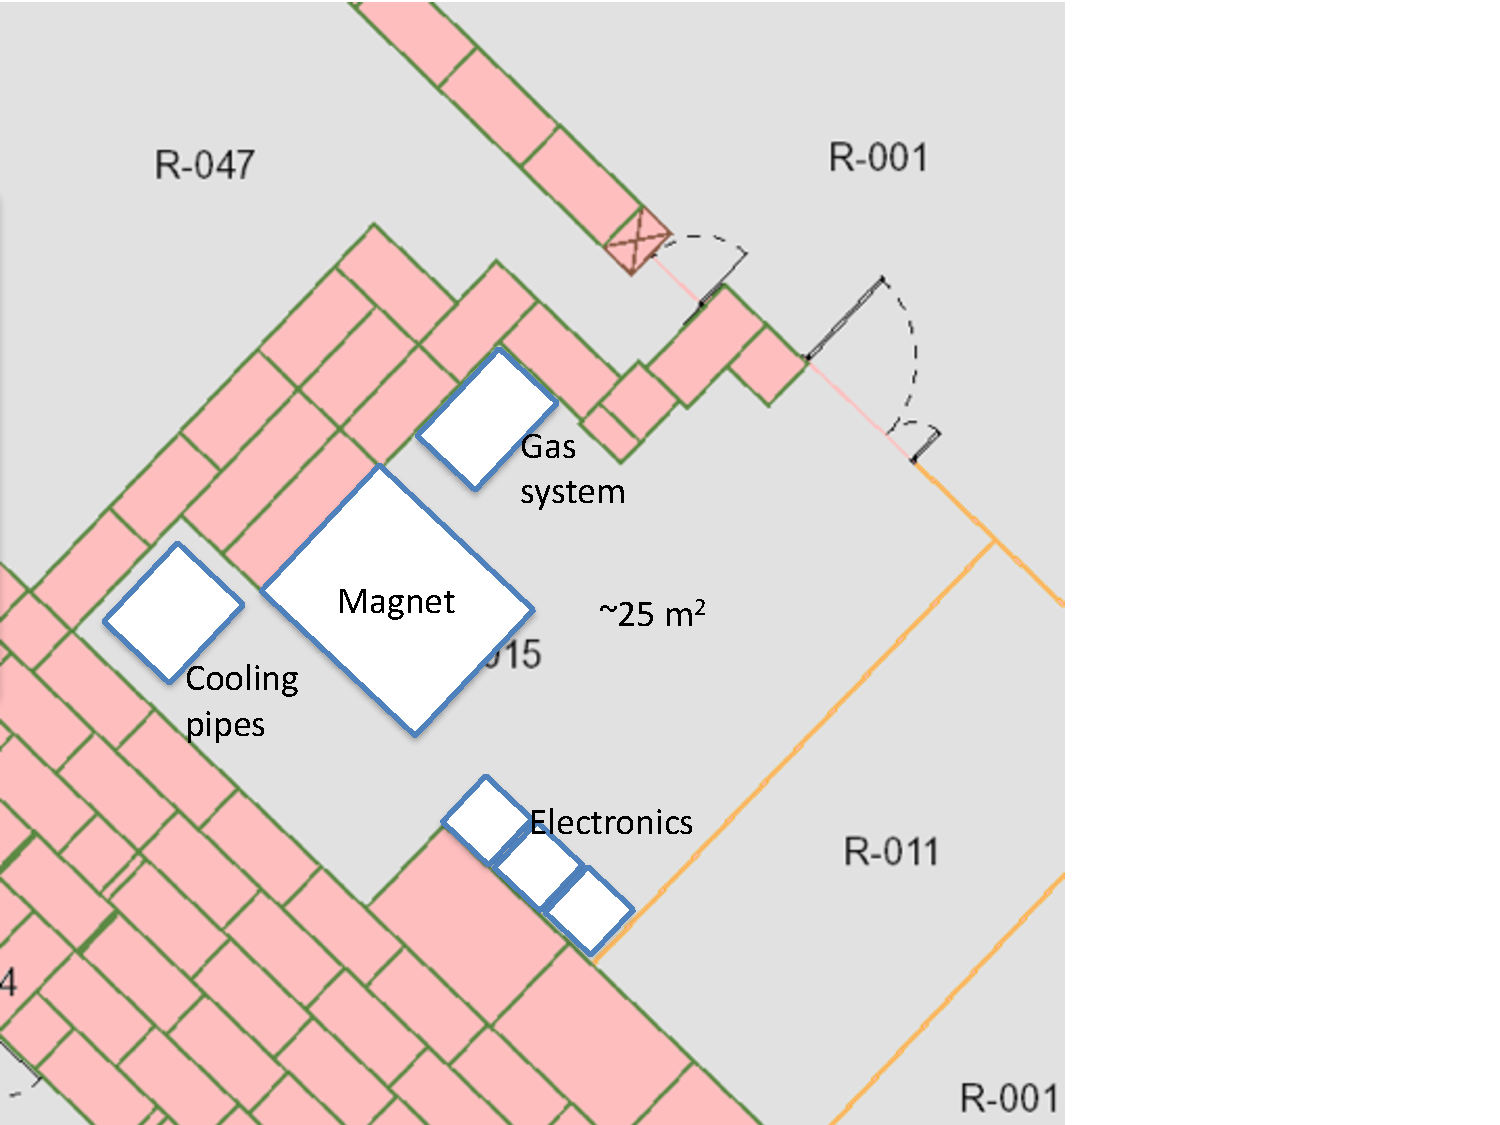
\includegraphics[angle=0,width=\textwidth]{img/distribution_examples.pdf}
\caption{Proposed distribution of the NEXT-DEMO, magnet and all different necessary systems for the operation of the detector in the experimental area} \label{fig:Distribution2}
\end{figure}


\begin{figure}
\centering
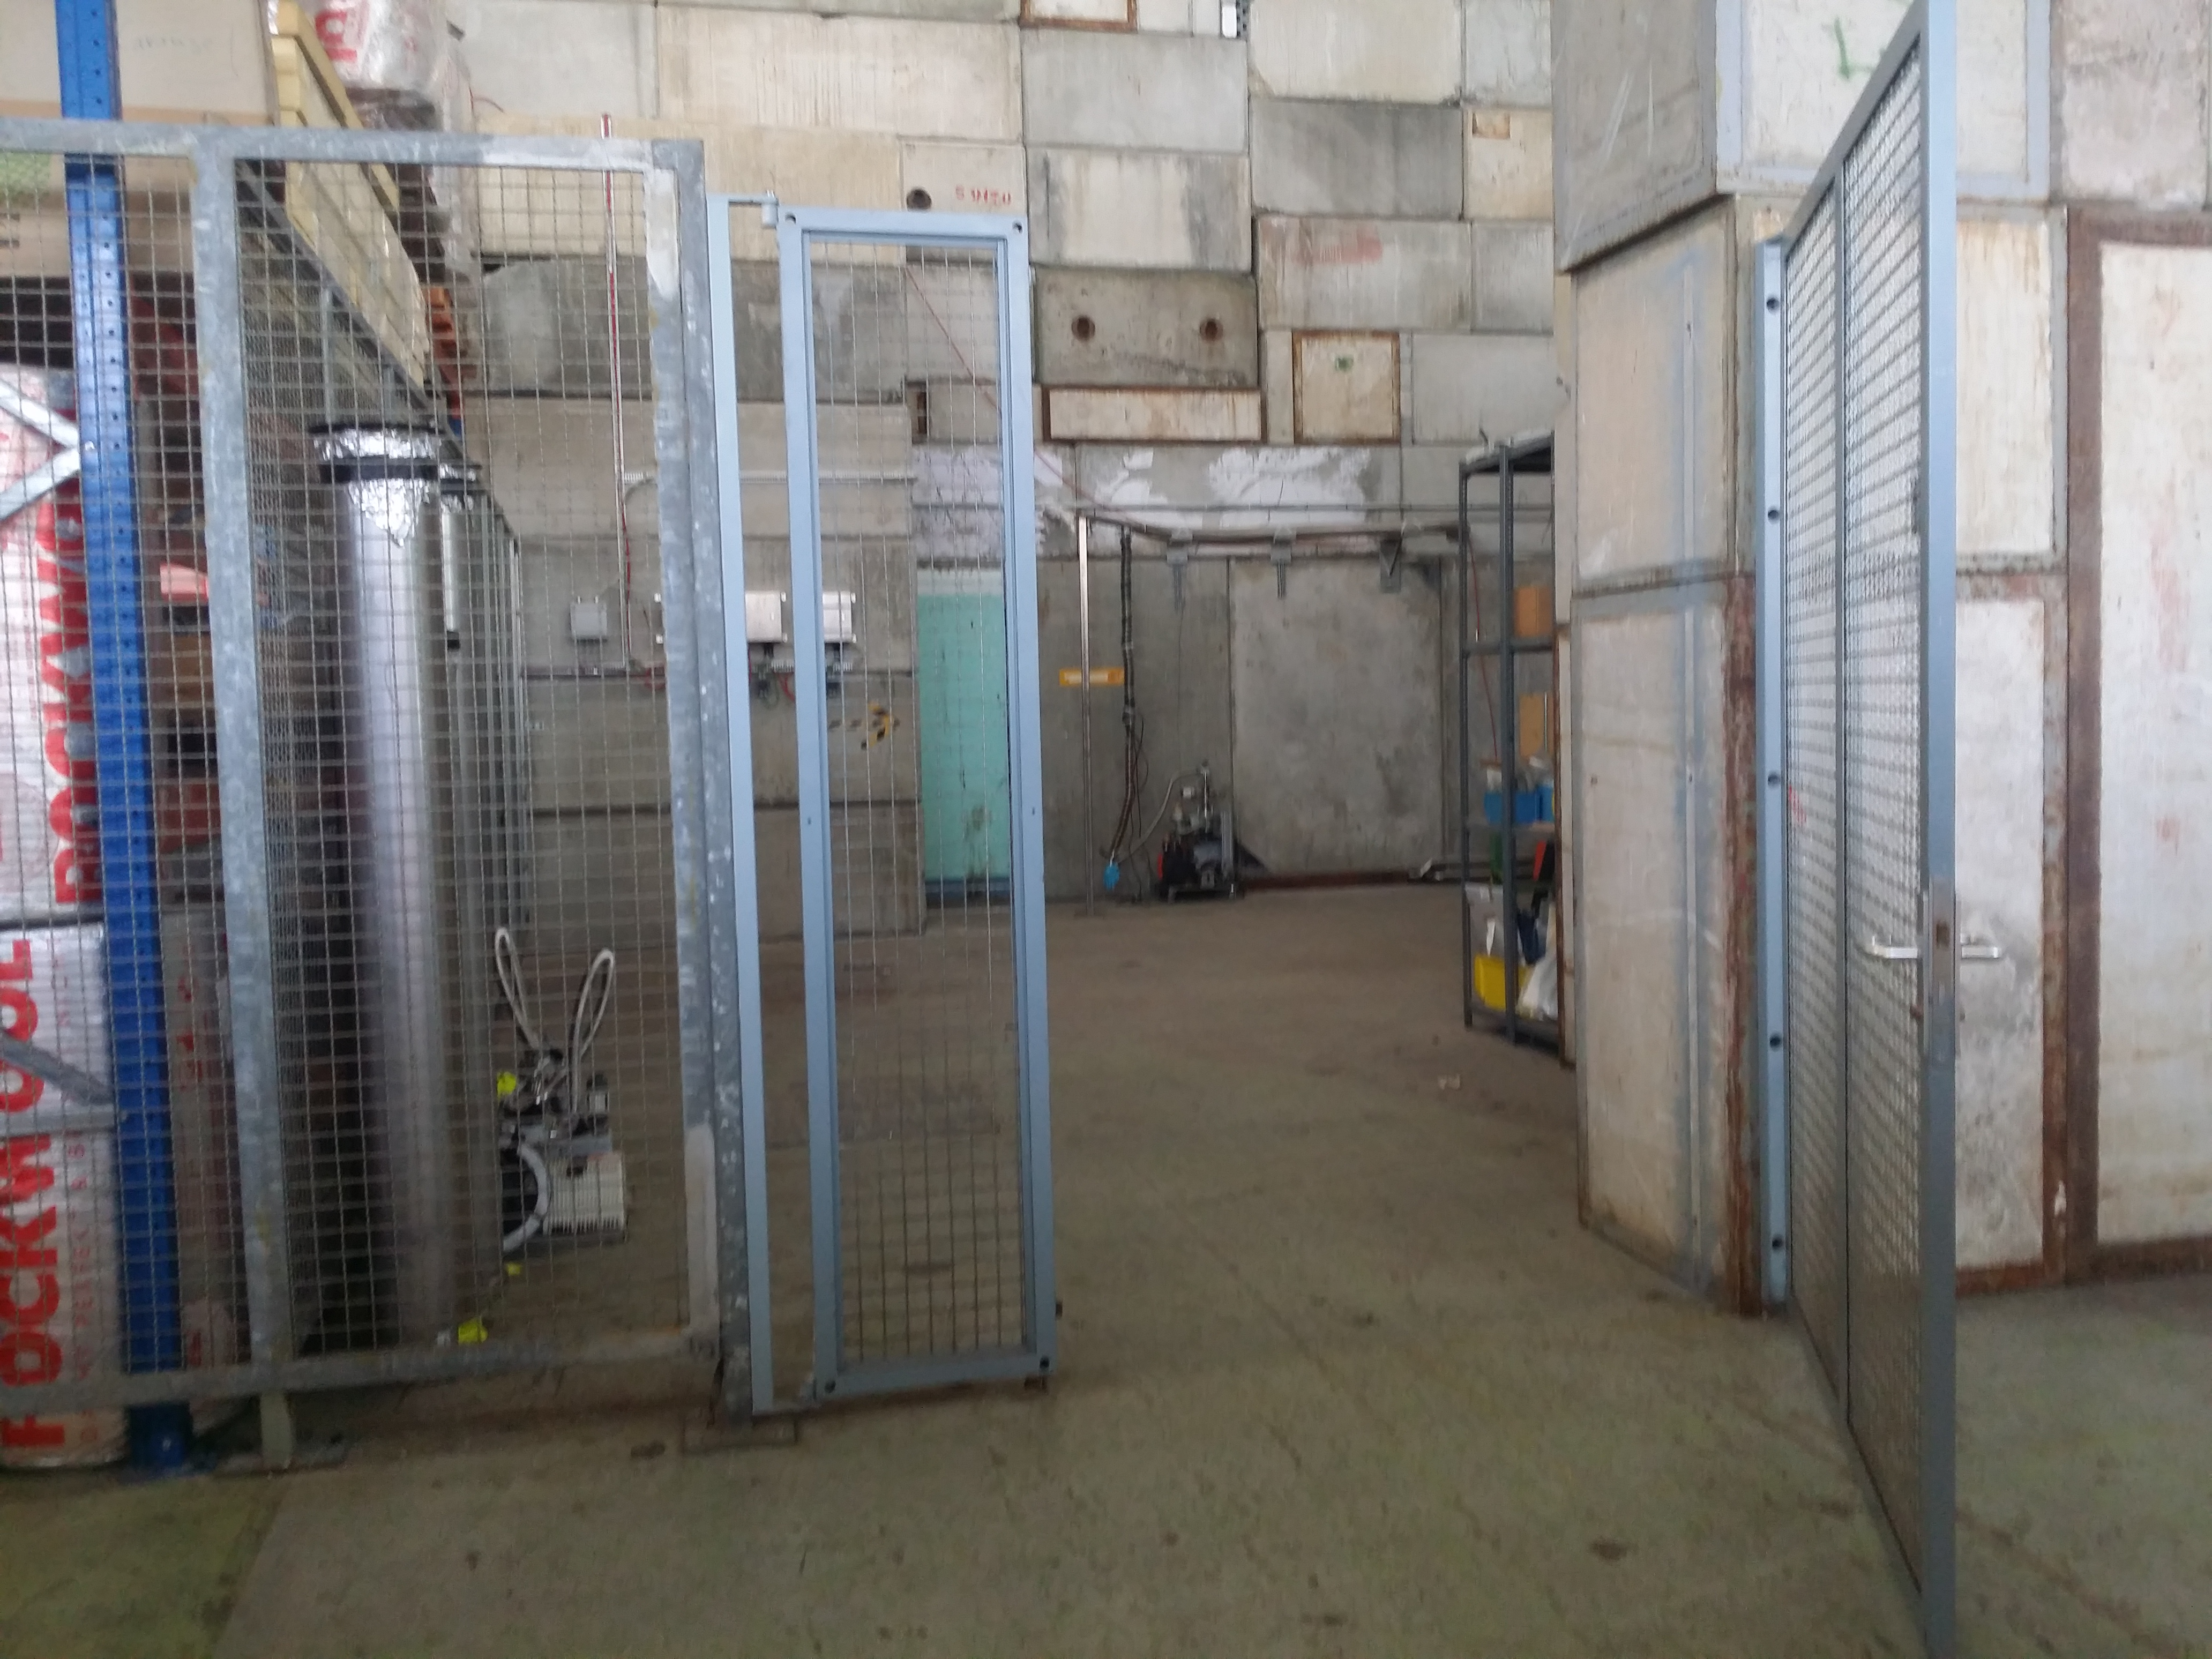
\includegraphics[width=0.45\textwidth]{img/experimentalarea1.jpeg}
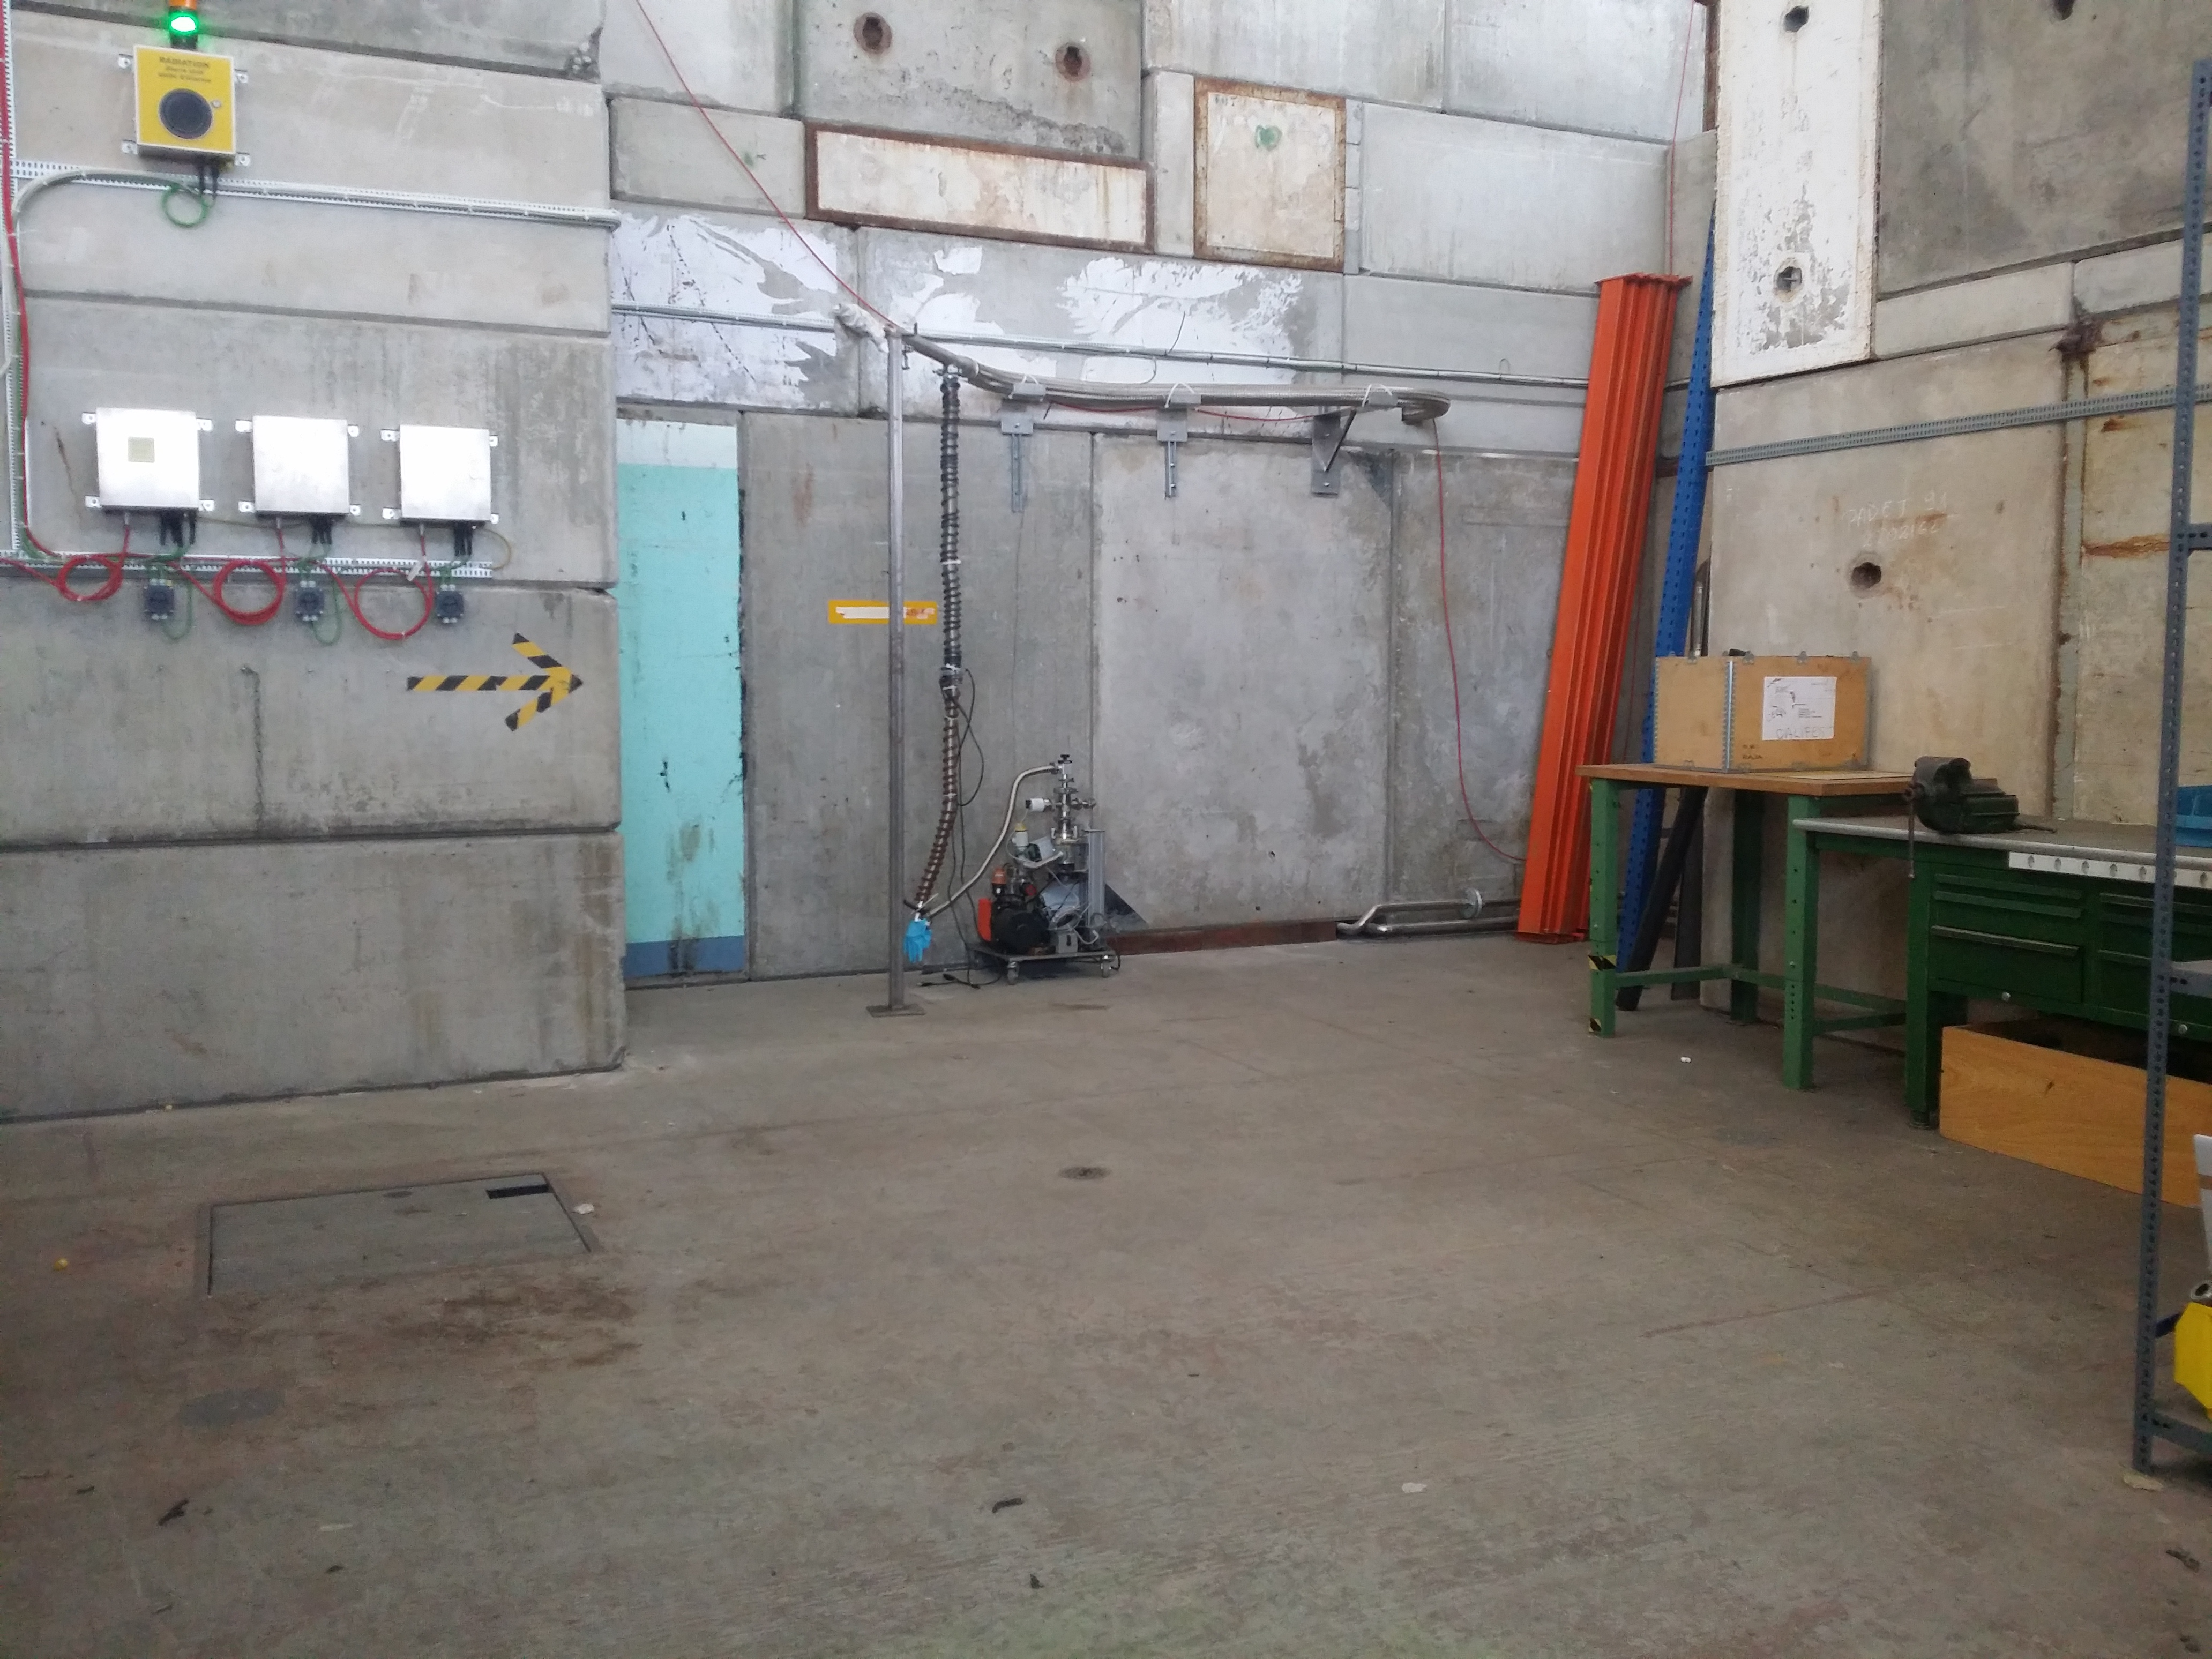
\includegraphics[angle=0,width=0.45\textwidth]{img/experimentalarea2.jpeg}
\caption{Proposed distribution of the NEXT-DEMO, magnet and all different necessary systems for the operation of the detector in the experimental area} \label{fig:pictures}
\end{figure}


\subsection{Related Gas systems}

Only one gas system will be used in the area. The gas system has been described in the main document. We recall that the amount of CO$_2$~needed is only of the order of 0.5 \% max, therefore, 5 grams for a xenon load of 1 kg (which is the operational load of DEMO++). Such small amount of gas only requires a bottle of 25 grams. We assume, however, a larger bottle of 100 grams which may be easier to handle. The following table summarizes the quantity and distribution of the different gases to be used in NEXT-DEMO:



\begin{table}[h]
%\resizebox{1.4\textwidth}{!}{\begin{minipage}{\textwidth}
\begin{tabular}{|r|r|r|r|r|}
\hline
\parbox[t]{2cm}{Gas Type} & \parbox[t]{3cm}{Supply description} & \parbox[t]{2cm}{Mass} &\parbox[t]{3cm}{ Volume (gas at ambient P ad T) }& \parbox[t]{3cm}{Supply location (see figure \ref{fig:Distribution2}) }\\\hline
Xenon & One bottle & 1500 g & 255 liters & GS 1  \\\hline
CO2 & One bottle & 100 g & 50 liters (approx.) & GS 1 \\\hline
\end{tabular}
\caption{Gas supply for NEXT-DEMO}
\label{tab:gassupply}
%\end{minipage} }
\end{table}

\subsection{Gas release risk assesment}

\subsubsection{Relevant Facts}
\begin{itemize}
\item All gases are at room temperature during normal operation.
\item A gas leak of the order of 1\% is easily detected.
\item All used gases are transparent and odorless.
\item All used gases are non-flamable. 
\end{itemize}

\subsubsection{Risk assesment}

\textit{Scenario 1}

A leak due to a crack in the gas system or the compressor, or due to an accidental impact that causes a hole in the system. The worst case scenario assumes that one of the pipes or flexible connection breaks. The largest pipes/flexibles in the system have a diameter of 1/2''. The result of such an event is a total, and very fast, loss of the gas.  

\textbf{Consequences:} In the above scenario, the gas is released at a flow of 2060 litres per minute, therefore, the total volume escapes in a few seconds. The slow control will detect the pressure dropped and take the following actions:
\begin{enumerate}
\item Stop the compressor.
\item Ramp down all the voltages. 
\item Activate an alarm in the experimental area. One could consider to include a second alarm in the underground galleries, although the risk appears to be negligible (see discussion below). 
\item Send electronic notification of failure to remote control systems.
\end{enumerate}

The associated hazard is the risk of asphyxiation due to the air being displaced by the released gas. Given that the area is open, the volume of CO$_2$ mould mix up in the air and would not posses any significant hazard. Xenon does not mix with air and tends to drop to floor level due to its weight. Since the area is open, xenon will also eventually diffused out of the area. 

To give an estimation of the worst case scenario we consider the case in which the area is assumed to be gas tight. In this case, the released volume (255 l) would occupy a surface of 25 m$^2$ and reach a height of 10.2 cm, which corresponds to the ankle of a normal height person. Since the area, far from being tight is fully open in one side, the gas will expand in a much larger area and pose no threat. 

A possible residual hazard would be that xenon leaks into the underground gallery of the power cables. However, the total volume is small, and will, again, diffuse very quickly. Nonetheless we propose to install an oxygen monitor in the area and another one in the entrance of the power cable gallery. Should those monitors (which will be connected to slow controls) detect any significant drop in the amount of oxygen, an alarm will be fired. 


\textit{Scenario 2}
 
 A leak occurs during cryogenic recovery of the Xenon. 
 
 \textbf{Consequences:} In this case the slow control will not respond to a drop of pressure. On the other hand, most of the Xenon should be frozen and the total volume of Xenon released to the atmosphere will be very small compared with the case previously considered. In any case, the presence of the oxygen monitors will guarantee safe operation. 
 

\subsection{Conclusions}

\subsubsection{Oxygen detection hazard}

It appears that CO$_2$~poses no risk whatsoever. The hazard associated with xenon release (asphyxiation) seems to be negligible even in the event of total and sudden release, given the fact that the experimental area is open and the total amount of gas is small. Nonetheless, we propose to install one Oxygen Detection Head (ODH) in the experimental area, and another one in the underground gallery connecting through which the power cables arrive. 

We propose the installation of three alarms (flashing red light and a a noise signal). One inside the experimental area, another one in the external part of the area, near the door and a third one in the underground gallery. 

\appendix 
\section{List of attachments}

This document is accompanied by a list of technical documents that reflect all the technical specifications and test performed in the gas system, pressure vessel and recovery bottles.

These documents are the following:
\begin{itemize}
%\item "VesselDrawings": It is a folder with the technical drawings used for the construction of the NEXT-DEMO pressure vessel.
%\item "PressureTest": This document is the certification of the pressure test realized for NEXT-DEMO.
%\item "XenonRecoveryBottles": This file contains the description of the recovery bottles for the Xenon, the engineering calculations and the results of the hidrostatic tests.
%\item "VALCI-MONT-195": It contains a detail description of all the elements used in the DEMO gas system.
%\item "PressureVesselCalculationsNEXTDEMO": This document presents the calculations of NEXTDEMO pressure vessel that has been designed to ASME pressure Vessel Design Code, sec VIII, division 1, the engineering drawings, the pictures of NEXTDEMO and the hysdrostatic test.

\item "Pressure Vessel" folder: It is a folder with the calculations, drawings and hidrostatic test performed for the construction fo the NEXT-DEMO pressure vessel.
\item "Gas System" older: It contains the technical description of the gas system (file VALCI-MONT-195.pdf), the data sheets of all different components of the gas system and the pneumatic test of the system.
\item "Recovery bottle" folder: It contains the information about the test of bottles for the cryo recovery.
\item "Cables and connections FUG" file: It provides information about the cables used for the high voltage.
\item "HAMEG-MAN-DE-EN-HMPSeries" file: It is the tecnical information for the power supply of the electronics.
\item "HHV Power Supplies" folder: It contains all the technical information related with the high voltage modules.

\end{itemize}





\end{document}
%
%
%%%%%%%%%%%%%%%%%%%%%%%%%%%%%%%%%%%%%%%%%%%%%%%%%%%%%%%%%%%%%
%\section{Time projection chamber} \label{sec:TPC}
%%%%
%Three metallic wire grids --- referred to as \emph{cathode}, \emph{gate} and \emph{anode} --- define the two active regions of the chamber (see figure~\ref{fig:TPC}): the 30 cm long \emph{drift region}, between cathode and gate; and the 0.5 cm long \emph{EL region}, between gate and anode. Gate and anode were built using stainless-steel meshes with 88\% open area (30-$\mu$m diameter wires, 50 wires$/$inch) clamped in a tongue-and-groove circular frame with a tensioning ring that is torqued with set screws to achieve the optimum tension. The cathode was built in a similar fashion by clamping parallel wires 1~cm apart into another circular frame.  
%
%%%%%%%%%%%
%\begin{figure}
%\centering
%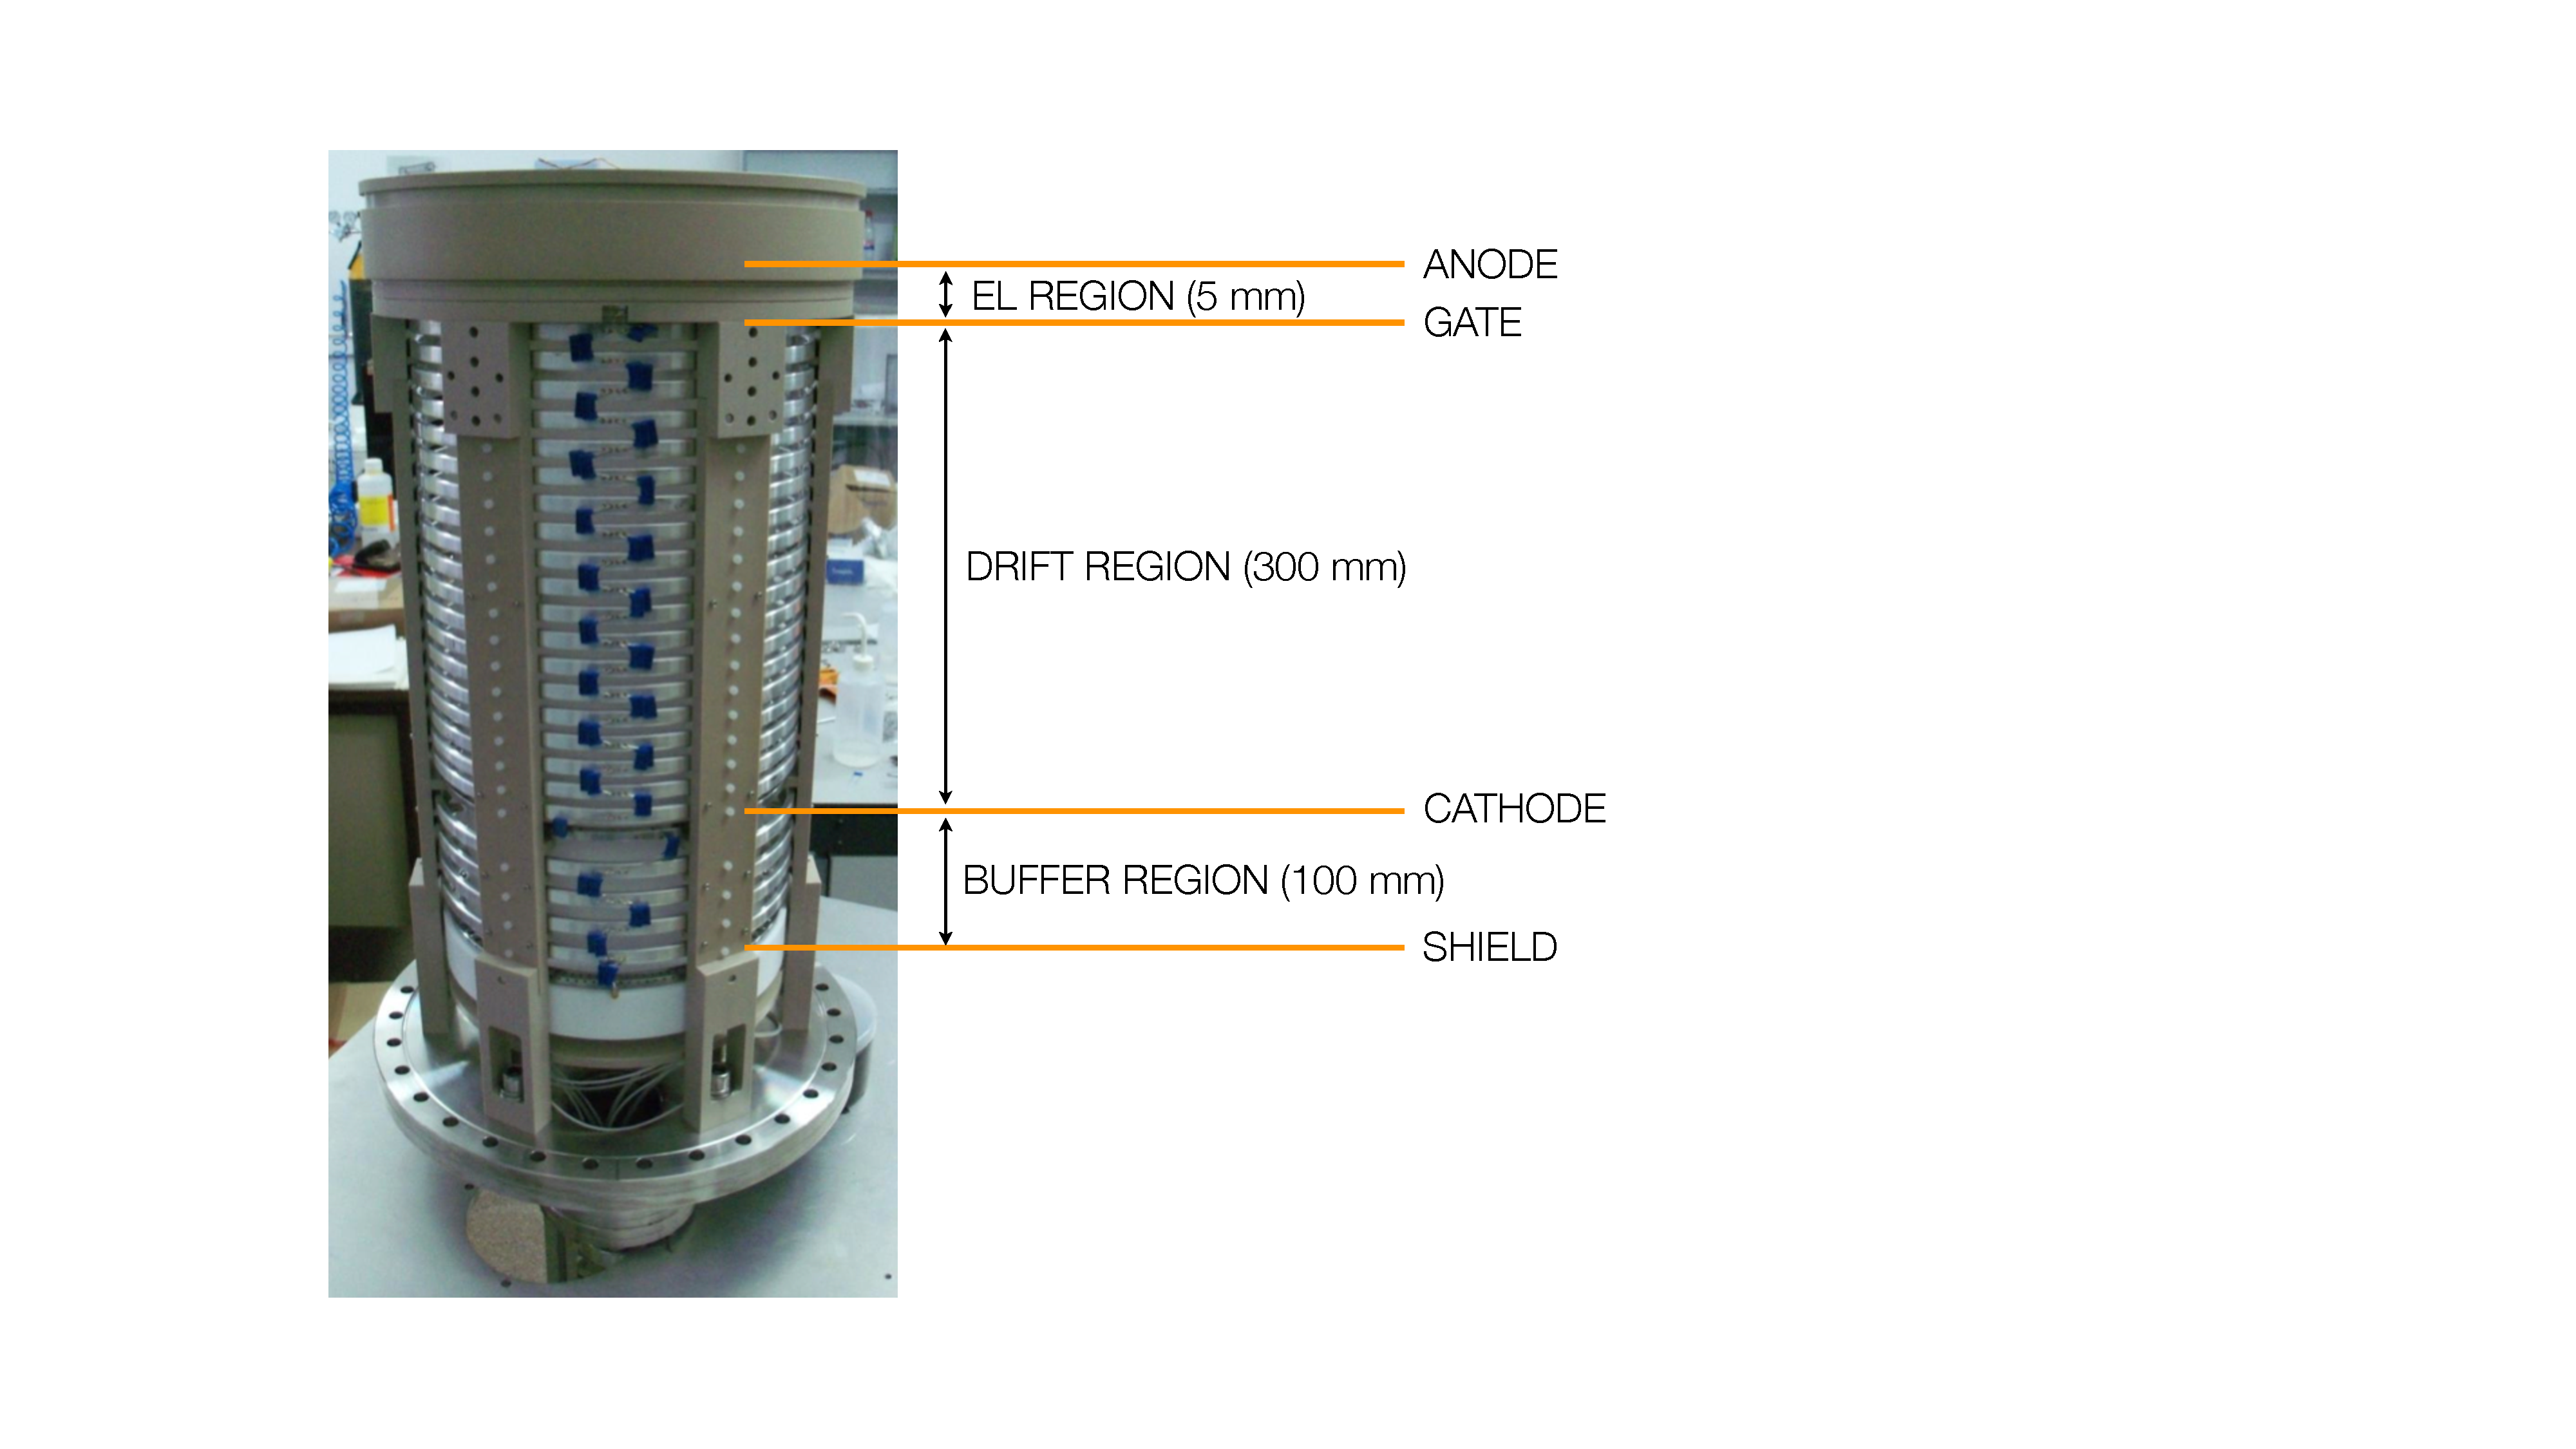
\includegraphics[width=0.75\textwidth]{img/FieldCage.pdf}
%\caption{External view of the time projection chamber mounted on one end-cap. The approximate positions of the different regions of the TPC are indicated.} \label{fig:TPC}
%\end{figure}
%%%%%%%%%%%
%
%The electric field in the TPC is created by supplying a large negative voltage to the cathode then degrading it across the drift region using a series of metallic rings of 30 cm diameter spaced 5 mm apart and connected via 0.5~G$\Omega$ resistors. The rings were manufactured by cutting and machining aluminum pipe. The gate is at negative voltage so that a moderate electric field --- typically of 2.5 to 3 $\mathrm{kV~cm^{-1}~bar^{-1}}$ --- is created between the gate and the anode, which is at ground.
%A \emph{buffer region} of 10 cm between the cathode and the energy plane protects this from the high-voltage by degrading it safely to ground potential.
%
%The high voltage is supplied to the cathode and the gate through custom-made high-voltage feed-throughs (HVFT), shown in figure~\ref{fig:HVFT}, built pressing a stainless-steel rod into a Tefzel (a plastic with high dielectric strength) tube, which is then clamped using plastic ferrules to a CF flange. They have been tested to high vacuum and 100 kV without leaking or sparking. 
%
%%%%%%%%%%%
%\begin{figure}
%\centering
%\includegraphics[scale=.7]{img/HVFT.jpg} 
%\caption{The NEXT-DEMO high-voltage feed-through, designed and built by Texas A\&M.}
%\label{fig:HVFT}
%\end{figure}
%%%%%%%%%%%
%
%A set of six panels made of PTFE (Teflon) are mounted inside the electric-field cage forming a \emph{light tube} of hexagonal cross section (see figure~\ref{fig:LightTube}) with an apothem length of 8 cm. PTFE is known to be an excellent reflector in a wide range of wavelengths \cite{Silva:2009ip}, thus improving the light collection efficiency of the detector. In a second stage, the panels were vacuum-evaporated with TPB --- which shifts the UV light emitted by xenon to blue ($\sim430$~nm) --- in order to study the  improvement in reflectivity and light detection. Figure~\ref{fig:LightTube} (bottom panel) shows the light tube illuminated with a UV lamp after the coating.
%
%%%%%%%%%%%
%\begin{figure}
%\centering
%\includegraphics[height=6.75cm]{img/LightTube.jpg}
%\includegraphics[height=6.75cm]{img/LightTubeBlue.JPG}  
%\caption{View of the light tube from the position of the tracking plane. Top: The meshes of the EL region can be seen in the foreground, and in the background, at the end of the light tube, the PMTs of the energy plane are visible. Bottom: The light tube of NEXT-DEMO illuminated with a UV lamp after being coated with TPB.} \label{fig:LightTube}
%\end{figure}
%%%%%%%%%%%
%
%Six bars manufactured from PEEK, a low outgassing plastic, hold the electric-field cage and the energy plane together. The whole structure is attached to one of the end-caps using screws, and introduced inside the vessel with the help of a rail system. All the TPC structures and the HVFT were designed and built by Texas A\&M.
%
%
%%%%%%%%%%%%%%%%%%%%%%%%%%%%%%%%%%%%%%%%%%%%%%%%%%%%%%%%%%%%%
%%\section{Detection planes} \label{sec:DetPlanes}
%%%%
%%NEXT-DEMO has been operating under two different configurations for the tracking plane. One with a tracking plane with PMTs and a second one with SiPMs. For both configurations the energy plane was not altered using exactly the same PMTs.
%
%\section{Energy Plane}\label{sec:EnergyPlane}
%In NEXT-DEMO, the energy plane (see figure~\ref{fig:DEMO_EnergyPlane}) is equipped with 19 Hamamatsu R7378A photomultiplier tubes. These are 1-inch, pressure-resistant (up to 20 bar) PMTs with acceptable quantum efficiency ($\sim 15$\%) in the VUV region. The resulting photocathode coverage of the energy plane is about 39\%. The PMTs are inserted into a PTFE holder following a hexagonal pattern. A grid, known as \emph{shield} and similar to the cathode but with the wires spaced 0.5~cm apart, is screwed on top of the holder and set to 500 V. As explained above, this protects the PMTs from the high-voltage set in the cathode, and ensures that the electric field in the 10-cm buffer region is below the EL threshold.
%
%The PMTs are connected to custom-made electrical bases that are used as voltage dividers, and also allow the extraction of the signal induced in the PMTs. This requires a total of 38 cables inside the pressure vessel connected via feed-throughs.  
%
%
%%%%%%%%%%%
%\begin{figure}
%\centering
%\includegraphics[height=6.5cm]{img/EnergyPlane.jpg}
%%\includegraphics[height=6.5cm]{img/TrackingPlane.jpg}
%\caption{The energy plane of NEXT-DEMO equipped with 19 Hamamatsu R7378A PMTs. The wires in front of the PMTs are the so called "shield" to fix the voltage in front of the PMTs and protect them from the Cathode Voltage.} \label{fig:DEMO_EnergyPlane}
%\end{figure}
%%%%%%%%%%%
%
%The goals of the PMT plane are first to measure the energy of the events recorded as it is related with total amount of light detected by the PMTs; and second, to detect the primary scintillation signal produced by each event which is fundamental to position the event inside the field cage and can be used also as a trigger signal. More details about the energy measurements performed by the PMT plane are dscribed in chapter \ref{chap:DEMOPMTResults}.
%
%
%%%%%%%%%%%%%%%%%%%%%%%%%%%%%%%%%%%%%%%%%%%%%%%%%%%%%%%%%%%%%
%\subsection{Energy Plane Electronics} \label{sec:EnergyElectronics}
%%%%
%The two optical signals in the NEXT detector concept have very different scales, and the photomultipliers and their front-end electronics must be ready to handle both. Primary scintillation results in weak (a few photoelectrons per photomultiplier) and fast (the bulk of the signal comes in about 20 ns) signals, whereas the secondary scintillation --- that is, the EL-amplified ionization --- is intense (hundreds to thousands of photoelectrons per PMT) and slow (several microseconds long). 
%
%The gain of the PMTs in the NEXT-DEMO energy plane was adjusted to around $5\times10^6$ to place the mean amplitude of a single photoelectron pulse well above electronic system noise.
%
%%and approximately half that for the tracking plane since they record the direct secondary-scintillation light produced in the EL region and, as such, would have a higher probability of saturation at the same gain as those of the cathode.
%
%The PMTs produce fast signals (less than 5~ns wide) making the shaping of the detector output necessary so that during the digitization with the 40MHz ADC the signal is sampled well enough to have a good estimation of the charge. This process also performs the important function of eliminating high frequency noise.
%
%The design uses a single amplification stage based on a fully differential amplifier THS4511, which features low noise ($2~\mathrm{nV/\sqrt{Hz}}$) and provides enough gain to mantain the signal amplitude above the noise level after shaping in the following stage. Amplification is followed by a passive RC filter with a cut frequency of 800 kHz. This filtering obtains the desired effect of stretching the signal to allow the acquisition of many samples per single photo-electron.
%The front-end circuit for NEXT-DEMO was implemented in 7 channel boards and connected via HDMI cables to 12-bit 40-MHz digitizer cards. These digitizers are read out by the FPGA-based DAQ modules (FEC cards) that buffer, format and send event fragments to the DAQ PCs. As for the FEC card, the 16-channel digitizer add-in card was designed in a joint effort between CERN and the NEXT Collaboration within the RD-51 program \cite{Martoiu:2011}. These two cards are edge mounted to form a standard 6U220 mm Eurocard. An additional FEC module with a different plug-in card is used as trigger module. Besides forwarding a common clock and commands to all the DAQ modules, it receives trigger candidates from the DAQ modules, runs a trigger algorithm in the FPGA and distributes a trigger signal. The trigger electronics also accept external triggers for detector calibration purposes.
%
%
%
%\section{Tracking Plane}\label{sec:TrackingPlane}
%
%\subsection{Tracking Plane with PMTs}\label{subsec:TrackingPlanePMT}
%As mentioned already, the first tracking plane of the NEXT-DEMO detector also uses  19 Hamamatsu R7378A PMTs, as shown in figure~\ref{fig:TrackingPMTs}, but operated at lower gain. They are also held by a PTFE honeycomb, mirroring the energy plane. The PMT windows are located 2 mm away from the anode mesh. Position reconstruction is based on energy sharing between the PMTs, being therefore much better than the distance between PMTs (35 mm from center to center).
%
%Position reconstruction with PMTs was used in the first stages of the detector because it allowed for a much simpler commisioning and understanding of the energy plane, trigger and other aspects of the detector with $\sim10$ times less number of channels to debug. Of course, reconstruction of the topology in detail with PMTs is not possible but a good average position reconstruction is easily achieved (\ref{sec:EnergyResolution} ) and fiducialization of the events is  possible.
%
%
%
%%%%%%%%%%%
%\begin{figure}
%\centering
%%\includegraphics[height=6.5cm]{img/EnergyPlane.jpg}
%\includegraphics[height=6.5cm]{img/DEMO_TrackingPlane.jpg}
%\caption{The tracking plane of NEXT-DEMO in the PMTs configuration, equipped with 19 Hamamatsu R7378A PMTs.} \label{fig:TrackingPMTs}
%\end{figure}
%%%%%%%%%%%
%
%
%
%\subsection{Tracking plane with SiPMs}\label{subsec:TrackingPlaneSiPM}
%
%\begin{figure}
%  \begin{center}
%  \includegraphics[width=0.475\textwidth,height=5cm]{img/DICE_Front.jpeg}
%  \includegraphics[width=0.475\textwidth,height=5cm]{img/DICE_back.jpeg}
%  \includegraphics[width=0.475\textwidth,height=5cm]{img/DICE_Plane_General.jpeg}
%  \includegraphics[width=0.475\textwidth,height=5cm]{img/DICE_Coated.jpeg}
%  \end{center}
%  \caption{Details of the \textit{CuFlon}$^{\circledR}$ boards and their mounting in NEXT-DEMO.}
%  \label{fig:DICEs}
%\end{figure}
%The arguments discussed in section \ref{sec:TOPO} led to the choice of a tracking plane 
%for NEXT-DEMO instrumented with SiPMs at a sensor pitch of 1~cm. The plane consists of 256 Hamamatsu S10362-11-050P SiPMs distributed between 4 boards, each with 64 sensors (see figure~\ref{fig:DICEs}) and is positioned 2~mm behind the EL production region. The active area of a sensor is 1~mm$^2$ comprised of pixels of side 50~$\mu$m. Operating at a bias voltage of 73~V results in a gain of $\sim7.5x10^5$ at room temperature (precise calibration described in section~\ref{subsec:TrackCali}) and dark current at the level of 0.2-0.3 photoelectrons$~\mu$s$^{-1}$.
%
%The SiPMs are mounted on multilayer \emph{CuFlon$^{\circledR}$} PCBs (PTFE substrate with copper layers, gold plated). Each board is supplied with one bias voltage via a FPC (Flat Printed Circuit) kapton cable which also extracts the sensor signals and the readings of a thermister positioned next to the board. In order to maintain the nominal supply voltage of the sensors and reduce detector dead time, 4 tantalum capacitors are connected to each board and supply the sensors with the required voltage after read-out.
%
%
%\subsubsection{Coating}
%\label{sec:coating}
%Since the SiPMs are not directly sensitive at the emission wavelength of Xe (170~nm), it is necessary to use a wavelength shifting coating. TPB has been used since its emission properties match well with the sensitivity of the SiPMs and because it was used to coat the light tube. The SiPM PCBs (DICE boards) were coated to a TPB thickness of 0.1~mg~cm$^{-2}$ by evaporation under high vacuum using the techniques described in detail in~\cite{Alvarez:2012ub}. The peak of the emission spectrum of TPB (430~nm) matches the region of highest quantum efficiency of the SiPMs well and at the selected TPB thickness the transmittance of the shifted light is $> 96\%$ \cite{Alvarez:2012ub}. While higher transmittance is possible with a thinner coating, the variance of the effective conversion efficiency tends to increase. The thickness chosen is, as such, a good compromise between these two competing considerations. 
%%\begin{figure}
% % \begin{center}
%  %  \includegraphics[width=0.445\textwidth]{img/DICE_Coated.jpeg}
%  %\end{center}
%  %\caption{A DICE fluorescing under UV light.} 
%  %\label{fig:DICE_coated}
%%\end{figure}
%
%%JJ ---> discussion of 1 cm etc, should be rather clear from added section
